%                                     MMMMMMMMM        
%                                                                             
%  MMO    MM   MMMMMM  MMMMMMM   MM    MMMMMMMM   MMD   MM  MMMMMMM MMMMMMM   
%  MMM   MMM   MM        MM     ?MMM              MMM$  MM  MM         MM     
%  MMMM 7MMM   MM        MM     MM8M    MMMMMMM   MMMMD MM  MM         MM     
%  MM MMMMMM   MMMMMM    MM    MM  MM             MM MMDMM  MMMMMM     MM     
%  MM  MM MM   MM        MM    MMMMMM             MM  MMMM  MM         MM     
%  MM     MM   MMMMMM    MM   MM    MM            MM   MMM  MMMMMMM    MM
%
%
%            - META-NET Language White Paper | Galician content -
% 
% ----------------------------------------------------------------------------

\begin{document}

\maketitle

\null
\pagestyle{empty} 

\makefundingnotice

\pagenumbering{Roman} 
\setcounter{page}{5}
\pagestyle{scrheadings}

\cleardoublepage

% --------------------------------------------------------------------------
\bsection*{Prefacio --- Preface}

\begin{Parallel}[c]{78mm}{78mm}
\ParallelLText{\selectlanguage{catalan}
   Esta serie de libros brancos sobre a linguaxe está dirixida a xornalistas, políticos, comunidades lingüísticas, profesores de idiomas, e todos aqueles que teñen o desexo de crear unha verdadeira Europa plurilingüe.

Estes libros brancos fomentan o coñecemento sobre a tecnoloxía lingüística (TL) e o seu potencial. A cobertura e o uso de tecnoloxías lingüísticas en Europa varía dun idioma a outro. Como consecuencia, as accións precisas para dar apoio á investigación e o desenvolvemento varían, e os pasos a seguir dependen de diversos factores, tales como a complexidade da lingua ou a dimensión da súa comunidade.

META-NET afrontou este reto poñendo en marcha unha análise da situación actual das tecnoloxías e dos recursos lingüísticos. A análise céntrase en 23 linguas europeas oficiais e en varias linguas rexionais de relevancia. Os resultados da análise suxiren que en cada lingua existen moitas carencias significativas. A análise e avaliación detalladas da situación de cada unha das linguas por parte de expertos axudará a maximizar o impacto das tecnoloxías lingüísticas e a minimizar calquera risco asociado.

META-NET é unha Rede de Excelencia da Comisión Europea formada por 44 centros de investigación de 31 países. META-NET traballa con interesados de diversas áreas da sociedade, a industria e a investigación para xerar enfoques estratéxicos e producir un plan de investigación decisivo que mostre como, mediante a posta en marcha das tecnoloxías lingüísticas, estas carencias poden ser cubertas no ano 2020. 

Aquest llibre blanc forma part d'una sèrie que vol donar a coneixer les tecnologies del llenguatge i el seu potencial. S'adreça a periodistes, polítics, comunitats lingüístiques i educadors entre d'altres.
A Europa, la disponibilitat de tecnologies del llenguatge i el seu ús varia segons l’idioma. En conseqüència, les accions que es requereixen per reforçar la investigació i el desenvolupament d'aquestes tecnologies també són diferents per a cada idioma. Les accions necessàries depenen de molts factors, com ara la complexitat d'una llengua determinada o de la mida de la comunitat de parlants.

META-NET, una xarxa d'excel·lència finançada per la Comissió Europea, ha dut a terme una anàlisi de l’estat actual dels recursos i les tecnologies del llenguatge per a les 23 llengües oficials europees, així com per a d’altres idiomes importants a nivell nacional i regional a Europa. Els resultats d'aquesta anàlisi suggereixen que hi ha encara mancances significatives en la investigació necessària per a cada idioma. Una anàlisi més detallada i una avaluació experta de la situació actual han de contribuir a maximitzar l'impacte de noves investigacions. 

A novembre de 2011, META-NET es compon de 54 centres de recerca de 33 països (p.~\pageref{metanetmembers}) que estan treballant amb tots els agents implicats: comercials, agències de govern,  organitzacions de recerca, empreses de programari, proveïdors de tecnologia i universitats europees. Junts, estan treballant en una visió comuna de la tecnologia i desenvolupant una agenda estratègica de la recerca que mostra com les aplicacions de les tecnologies del llenguatge podran resoldre els problemes actuals abans de l’any 2020.

}

\ParallelRText{\selectlanguage{english}
This white paper is part of a series that promotes knowledge about language technology and its potential. It addresses journalists, politicians, language communities, educators and others. 
The availability and use of language technology in Europe varies between languages. Consequently, the actions that are required to further support research and development of language technologies also differ. The required actions depend on many factors, such as the complexity of a given language and the size of its community.

META-NET, a Network of Excellence funded by the European Commission, has conducted an  analysis of current language resources and technologies in this white paper series (p.~\pageref{whitepaperseries}). The analysis focused on the 23 official European languages as well as other important national and regional languages in Europe. The results of this analysis suggest that there are tremendous deficits in technology support and significant research gaps for each language. The given detailed expert analysis and assessment of the current situation will help maximise the impact of additional research.

As of November 2011, META-NET consists of 54 research centres from 33 European countries (p.~\pageref{metanetmembers}). META-NET is working with stakeholders from economy (software companies, technology providers and users), government agencies, research organisations, non-governmental organisations, language communities and European universities. Together with these communities, META-NET is creating a common technology vision and strategic research agenda for multilingual Europe 2020.} 
\ParallelPar
\end{Parallel}

\cleardoublepage

% --------------------------------------------------------------------------
\bsection*{Sumari --- Table of Contents}

\renewcommand\contentsname{}

\tableofcontents
\addtocontents{toc}{\protect\thispagestyle{empty}\protect}
\addtocontents{toc}{{\Large\textsf{\centerline{La LLENGUA CATALANA A L'ERA DIGITAL}}\par}}

\cleardoublepage


% --------------------------------------------------------------------------
\setcounter{page}{1}
\pagenumbering{arabic} 
\pagestyle{scrheadings}


% Start of origin language part
% --------------------------------------------------------------------------
\ssection[Resum]{Resum}

\selectlanguage{catalan}

\begin{multicols}{2}

Durante os últimos 60 anos, Europa converteuse nunha estrutura política e económica ben definida, aínda que tanto a nivel cultural como lingüístico continúa a ser moi diversa; é dicir, que a comunicación entre cidadáns europeos, tanto a máis cotiá como a que se produce no eido dos negocios ou a política, ben sexa en portugués como en polaco, en italiano o en islandés, vese confrontada inevitablemente polas barreiras do idioma. As institucións da UE gastan preto de mil millóns de euros ao ano para manter a súa política de plurilingüismo, é dicir, na tradución de textos e a interpretación de comunicacións orais. Mais, é preciso que a diversidade lingüística resulte unha carga tan custosa? As modernas tecnoloxías da linguaxe e a investigación lingüística poden contribuír de maneira significativa a eliminar estas barreiras lingüísticas. Combinando axeitadamente os dispositivos intelixentes e as súas aplicacións con estas tecnoloxías da linguaxe poderase, nun futuro, axudar aos cidadáns europeos a comunicarse facilmente os uns cos outros e establecer unha relación comercial a pesar de non falar unha lingua común. 

    \boxtext{A tecnoloxía da linguaxe constrúe pontes para o futuro de Europa}

A economía europea saca un maior proveito do mercado único europeo que dos outros: no ano 2010, o comercio dentro da UE representaba o 60,3\% das exportacións alemás, mentres que o comercio con outros países europeos ascendía a un 10,8\%. Non obstante, as barreiras lingüísticas poden parar o progreso dos negocios, especialmente no caso das PEMES que non teñen os medios económicos para facer fronte a esta situación. A única alternativa (impensable, por outra banda) a esta Europa plurilingüe sería permitir que unha única lingua tomase unha posición dominante e rematase por substituír todas as demais linguas.

Unha forma clásica de superar as barreiras lingüísticas é a aprendizaxe de linguas estranxeiras, mais, con falta de apoio tecnolóxico, dominar as 23 linguas oficiais dos Estados membros da Unión Europea e aproximadamente outras 60 linguas europeas adicionais, é unha tarefa practicamente imposible para calquera cidadán, así como un freo para o desenvolvemento económico, o debate político ou o progreso científico de Europa.

A solución pasa por desenvolver tecnoloxías clave que faciliten a comunicación. Estas tecnoloxías ofrecen vantaxes enormes no ámbito europeo, non só dentro do mercado común, senón tamén nas relacións comerciais con terceiros países, especialmente os que contan con economías emerxentes. Para acadar este obxectivo e preservar a diversidade cultural e lingüística de Europa, primeiro é necesario realizar unha análise sistemática das particularidades lingüísticas e o estado actual da tecnoloxía lingüística de apoio de cada un dos idiomas europeos. Nun futuro, as solucións das tecnoloxías da linguaxe poderán servir de ponte entre as linguas de Europa.

A tradución automática e as ferramentas de procesamento da fala actualmente dispoñibles no mercado aínda están lonxe dun obxectivo tan ambicioso. Os principais protagonistas neste ámbito son as empresas privadas con ánimo de lucro radicadas en Norteamérica. Xa na década de 1970, a UE decatouse da grande relevancia das tecnoloxías da linguaxe como factor impulsor da unidade europea, e comezou a financiar os seus primeiros proxectos de investigación, como por exemplo EUROTRA. Ao mesmo tempo, establecéronse proxectos nacionais que xeraron valiosos resultados, pero nunca chegaron a constituír unha acción europea coordinada. Fronte a este esforzo de financiamento selectivo, outras sociedades plurilingües, como a India (con 22 linguas oficiais) e Sudáfrica (con 11 linguas oficiais) crearon recentemente programas nacionais de investigación lingüística e desenvolvemento tecnolóxico a longo prazo.

Hoxe en día, os modelos predominantes nas tecnoloxías da linguaxe dependen de métodos estatísticos que non fan uso de métodos ou coñecementos lingüísticos profundos. Por exemplo, as frases tradúcense automaticamente mediante a comparación dunha nova frase con miles de frases previamente traducidas por humanos. A calidade da tradución depende en gran medida da cantidade e calidade dos corpus de mostra dispoñibles. Mentres que a tradución automática de oracións simples en idiomas cunha cantidade suficiente de material textual dispoñible pode dar resultados útiles, os métodos estatísticos están condenados ao fracaso no caso de idiomas cun material de mostra moito máis pequeno, ou no caso da tradución de oracións con estruturas complexas.

\boxtext{Tecnoloxía da linguaxe como clave para o futuro}

A Unión Europea decidiu financiar proxectos como EuroMatrix e EuroMatrixPlus (dende o ano 2006) e iTranslate4 (dende 2010), que  levan a cabo unha investigación básica e aplicada e crean recursos para o establecemento de solucións de alta calidade en tecnoloxías da linguaxe para todos os idiomas europeos. A análise das propiedades estruturais máis profundas das linguas é o único camiño a seguir se queremos crear aplicacións que funcionen ben en toda a variedade de linguas de Europa. A investigación europea neste ámbito xa acadou varios éxitos. Por exemplo, os servizos de tradución da Unión Europea empregan agora MOSES, un software de tradución automática de código fonte que foi desenvolvido principalmente grazas a proxectos de investigación europeos. O proxecto Verbmobil, financiado polo ministerio alemán de Educación e Investigación (BMBF) entre os anos 1993 e 2000, situou a Alemaña á fronte do mundo da investigación en tradución da fala durante un tempo. Moitos dos laboratorios de investigación e desenvolvemento situados en Alemaña daquela (coma IBM ou Philips) foron pechando ou trasladáronse a outro lugar. No canto de basearse sobre os resultados dos seus proxectos de investigación, Europa tendeu a realizar actividades illadas con pouco impacto no mercado. O valor económico dos primeiros esforzos pódese ver mesmo no número de derivados posteriores. Unha compañía como Trados, que fora fundada no ano 1984, foi vendida á compañía SDL, con sede no Reino Unido, no ano 2005.

\boxtext{As tecnoloxías da linguaxe axudan a unificar Europa}

Segundo o estado actual das tecnoloxías da linguaxe, parece ser que as chamadas “tecnoloxías híbridas”, que combinan o procesamento a partir de coñecementos lingüísticos profundos con métodos estatísticos, serán capaces de conectar todas as linguas europeas e de moito máis. Como esta serie de libros brancos sobre as linguas europeas demostra, hai grandes diferenzas en canto a investimento en solucións tecnolóxicas e ao estado da investigación lingüística entre os Estados membros de Europa.  O galego é unha das linguas da UE que necesita aínda máis investigación para que as solucións das tecnoloxías da linguaxe cheguen a ser verdadeiramente eficaces e poidan ser empregadas para un uso diario. Ao mesmo tempo, existen boas perspectivas para acadar unha posición salientable nesta área tecnolóxica tan importante. A longo prazo, o obxectivo de METANET é introducir tecnoloxías da linguaxe de alta calidade para todos os idiomas co fin de conseguir unha unidade política e económica a través da diversidade cultural. A tecnoloxía axudará a eliminar as barreiras existentes e a construír pontes entre as linguas europeas. Isto require que todas as partes interesadas, tanto do eido da política, a investigación, as empresas e a sociedade unan os seus esforzos para o futuro.

Esta serie de libros brancos complementa outras accións estratéxicas adoptadas por META-NET (ver resumo no apéndice). As versións actualizadas dos documentos “\textit{META-NET vision paper}” \cite{Meta1} ou “\textit{Strategic Research Agenda (SRA)}” poden atoparse na páxina web de META-NET: \url{http://www.meta-net.eu}.
\end{multicols}

\clearpage


% --------------------------------------------------------------------------
\ssection[Un risco para as nosas linguas e un reto para a tecnoloxía lingüística]{Un risco para as nosas linguas\newline e un reto para \newline a tecnoloxía lingüística}

\begin{multicols}{2}

 Estamos a presenciar  unha revolución dixital que ten importantes repercusións nas comunicacións e na sociedade. Os recentes avances na tecnoloxía da comunicación dixital e en rede equipáranse ás veces coa invención da imprenta de Gutenberg. Que é o que nos di esta analoxía sobre o futuro da sociedade europea da información y das nosas linguas en particular? 


\boxtext{***HELPThe digital revolution is comparable to Gutenberg’s invention of the printing press.***FHELP}

Tras a invención de Gutenberg, acadáronse grandes avances na comunicación e no intercambio de coñecemento grazas a esforzos como a tradución de Lutero da Biblia á lingua común. Nos séculos posteriores, desenvolvéronse técnicas culturais para unha mellor xestión do procesamento da linguaxe e do intercambio de coñecemento:
\begin{itemize}
\item a normativización ortográfica e gramatical dos principais idiomas permitiu unha rápida difusión de novas ideas científicas e intelectuais;
\item a evolución dos idiomas oficiais fixo posible que os cidadáns se puidesen comunicar dentro de certas fronteiras (a miúdo políticas);
\item o ensino e a tradución das linguas permitiu un intercambio entre idiomas;
\item a creación de directrices xornalísticas e bibliográficas asegurou a calidade e dispoñibilidade do material impreso;
\item a creación de diferentes medios de comunicación como os xornais, a radio, a televisión, os libros, e outros formatos, satisfixeron as distintas necesidades comunicativas. 
\end{itemize}
Nos últimos vinte anos, a tecnoloxía da información, ou informática, veu axudando á hora de automatizar e facilitar moitos procesos:
\begin{itemize}
\item os programas informáticos de autoedición substitúen á mecanografía e á redacción;
\item Microsoft PowerPoint substitúe ás transparencias nos retroproxectores;
\item o correo electrónico envía e recibe documentos habitualmente máis rápido cás máquinas de fax; 
\item Skype permite realizar chamadas telefónicas vía Internet e organizar reunións virtuais;
\item os formatos de codificación de audio e vídeo facilitan o inter-cambio de contidos multimedia;
\item os motores de busca proporcionan acceso ás páxinas web baseándose en palabras clave;
\item os servizos en liña, como o tradutor de Google, realizan traducións rápidas e aproximadas;
\item as plataformas sociais multimedia facilitan a colaboración e o intercambio de información.
\end{itemize}
A pesar de que moitas destas ferramentas e aplicacións resultan moi útiles, son suficientes para poñer en marcha unha sociedade europea da información plurilingüe, unha sociedade moderna e global onde a información e os bens poidan circular libremente?

\subsection{As fronteiras lingüísticas obstaculizan á sociedade da  información europeai}
  
 Non podemos predicir con exactitiude como será a sociedade da información no futuro, mais é moi probable que a revolución da tecnoloxía da comunicación achegue, de novas maneiras, ás persoas que falan diferentes idiomas. Isto provoca que a xente se vexa cada vez máis obrigada a aprender novos idiomas, e os programadores máis obrigados a crear novas aplicacións tecnolóxicas que garanticen un entendemento mutuo e un acceso ao coñecemento compartido. Nun contorno de economía global e espazo de información, vémonos expostos a máis idiomas, falantes e contidos, e isto require que sexamos capaces de interactuar con rapidez cos novos medios de comunicación. A actual popularidade das plataformas sociais multimedia (Wikipedia,  \textit{Facebook}, \textit{Twitter}  e \textit{YouTube}) e só a punta do iceberg.


\boxtext{***HELPThe global economy and information space confronts us with different languages, speakers and content.***FHELP}


Hoxe en día podemos transmitir xigabytes de texto por todo o mundo en cuestión de segundos antes de que recoñezamos que está nun idioma que non comprendemos. Segundo un informe recente solicitado pola Comisión Europea, o 57\% dos usuarios de Internet en Europa mercan bens e servizos en idiomas diferentes aos seus idiomas nativos. (O inglés é a lingua estranxeira máis común, seguida do francés, o alemán e o español). O 55\% de usuarios le contidos en idiomas estranxeiros, mais só un 35\% empregan outra lingua para escribir correos electrónicos ou deixar comentarios na web \cite{GAL-Nota1}.  Hai uns anos, o inglés podía ser considerado a lingua vehicular da Internet, xa que a grande maioría dos seus contidos estaban escritos neste idioma. Non obstante, a situación actual é moi diferente. A cantidade de contido que aparece na Internet noutros idiomas (especialmente idiomas asiáticos e árabes) disparouse.

Sorprendentemente, no debate social non se lle prestou demasiada atención á brecha dixital ubicua causada polas fronteiras lingüísticas; así e todo, isto presenta unha cuestión urxente: "que idiomas europeos prosperarán e persistirán na información en rede e na sociedade do coñecemento?"

\subsection{As nosas linguas en perigo}

    A imprenta contribuíu a un intercambio moi valioso de información en Europa, pero tamén levou consigo a extinción de moitos idiomas europeos. Raras veces se imprimía nas linguas rexionais e minoritarias. Como resultado, moitos idiomas, como o córnico ou o dálmata, víronse limitados á transmisión oral, o cal restrinxiu a súa adopción, difusión e uso continuados.***HELP Will the Internet have the same impact on our languages? ***FHELP

\boxtext  {The variety of languages in Europe is one of its richest and most important cultural assets.}
***FHELP

As aproximadamente 80 linguas que existen en Europa son un dos seus bens culturais máis ricos e importantes. A multitude de idiomas de Europa constitúe un elemento fundamental do seu éxito social \cite{GAL-Nota2}. Mentres que outros idiomas populares, como o inglés ou español, manterán de seguro a súa presenza na sociedade e no mercado dixital emerxente, moitos idiomas europeos poderían verse illados a causa das comunicacións dixitais e poderían chegar a converterse en idiomas irrelevantes na sociedade da Internet. Isto debilitaría a posición global de Europa, e entraría en conflito co obxectivo estratéxico de asegurar a participación igualitaria de cada cidadán europeo, independentemente do seu idioma. Segundo un informe da UNESCO sobre o plurilingüismo, os idiomas son un medio imprescindible para o gozo dos dereitos fundamentais, tales como a expresión política, a educación, e a participación na sociedade \cite{GAL-Nota3}.

\subsection{A tecnoloxía lingüística é unha tecnoloxía instrumental clave}

   No pasado, as inversións centrábanse no ensino de idiomas e na súa tradución. Por exemplo, segundo algunhas estimacións, o mercado europeo para a tradución, a interpretación, a localización de \textit{software}, e a globalización das páxinas web era, no ano 2008, de 8,4 miles de millóns de euros, e esperábase un crecemento dun 10\% anual \cite{GAL-Nota4}.  Non obstante, estes recursos existentes non son suficientes para satisfacer as necesidades actuais e as futuras. 

A tecnoloxía lingüística ***HELP (targeting all forms of written text and spoken discourse) ***FHELP permite que os cidadáns colaboren, fagan negocios, compartan coñecementos, e participen nos debates sociais e políticos independentemente das barreiras lingüísticas ou dos coñecementos informáticos.  ***HELP It often operates invisibly inside complex software systems to help us:***FHELP
	\begin{itemize}
	   \item buscamos e traducimos páxinas web;  
	   \item empregamos as opcións de corrección gramatical e ortográfica nos procesadores de texto;
	   \item lemos as recomendacións dun produto nunha tenda \textit{online};
	   \item escoitamos as instrucións verbais dunha voz sintética nun sistema de navegación; 
	   \item traducimos páxinas web cun servizo \textit{online}.
	\end{itemize}
As tecnoloxías lingüísticas detalladas neste informe constitúen unha parte fundamental das futuras aplicacións innovadoras. A tecnoloxía lingüística é, polo xeral, unha tecnoloxía instrumental que se sitúa dentro dun marco de aplicación máis amplo, como un sistema de navegación ou un motor de busca. Estes libros brancos céntranse na capacidade das tecnoloxías básicas en cada lingua. 


***HELP \boxtext{Europe needs robust and affordable language technology for all European languages.} ***FHELP

Nun futuro próximo, necesitaremos que estea dispoñible unha tecnoloxía lingüística para todas as linguas europeas, que sexa economicamente alcanzable e que se atope perfectamente integrada dentro duns ámbitos informáticos máis amplos. Sen a tecnoloxía lingüística, non se pode acadar unha experiencia interactiva, multimedia e plurilingüe dos usuarios. 

\subsection{Oportunidades para a tecnoloxía lingüística}

 ***HELP
   In the world of print, the technology breakthrough was the rapid duplication of an image of a text (a page) using a suitably powered printing press. Human beings had to do the hard work of looking up, reading, translating, and summarizing knowledge. We had to wait until Edison to record spoken language – and again his technology simply made analogue copies. ***FHELP

    A tecnoloxía lingüística fai posible a a tradución automática, a produción de contidos, o procesamento da información e a xestión do coñecemento para todos os idiomas europeos. A tecnoloxía lingüística tamén pode potenciar o desenvolvemento de interfaces lingüísticas intuitivas para os electrodomésticos, a maquinaria, os vehículos, os ordenadores e os robots. A pesar de que xa existen moitos prototipos, as aplicacións comerciais e industriais aínda están nas primeiras fases do desenvolvemento. O ritmo actual do progreso presenta unha verdadeira oportunidade, tendo en conta que a investigación veu progresando de maneira constante durante os últimos anos. Por exemplo, a tradución automática (TA) hoxe en día é capaz de proporcionar unha precisión bastante aceptable en certos ámbitos específicos, e as aplicacións experimentais ofrecen unha xestión da información e o coñecemento plurilingüe, así como unha produción de contidos en moitas linguas europeas. 

As aplicacións lingüísticas, as interfaces de usuario baseadas en voz, e os sistemas de diálogo adoitan atoparse en ámbitos altamente especializados, e a miúdo mostran un rendemento limitado. Existen grandes oportunidades de mercado nas industrias da educación e do espectáculo para a integración das tecnoloxías lingüísticas en xogos, ofertas de lecer educativo, o ámbito da simulación ou programas de formación. Os servizos de información móbil, os programas de aprendizaxe de idiomas asistidos por ordenador, os ámbitos de aprendizaxe electrónica, as ferramentas de autoavaliación, e os programas de detección de plaxio son só uns cantos exemplos máis onde a tecnoloxía lingüística pode desempeñar un papel importante. A popularidade de aplicacións sociais multimedia, como Twitter e Facebook, suxiren unha necesidade de tecnoloxías lingüísticas sofisticadas que poidan supervisar as publicacións, resumir os debates, indicar as opinións públicas, detectar as respostas emocionais, identificar as violacións dos dereitos de autor, ou facer un seguimento de uso indebido.

 ***HELP \boxtext{Language technology helps overcome the “disability” of linguistic diversity.} ***FHELP

A tecnoloxía lingüística representa unha grande oportunidade para a Unión Europea que non se aplica só a nivel económico senón tamén a nivel cultural. O plurilingüismo en Europa converteuse na regra. As empresas, organizacións e escolas europeas tamén son multinacionais e diversas. Os cidadáns queren comunicarse máis aló das fronteiras lingüísticas que aínda existen no Mercado Común europeo. A tecnoloxía lingüística pode axudar a superar estas barreiras aínda existentes, defendendo á vez un uso libre e aberto da linguaxe. Ademais, unha tecnoloxía lingüística plurilingüe e innovadora para Europa pode tamén axudarnos a comunicarnos cos nosos socios globais e as súas comunidades plurilingües. As tecnoloxías lingüísticas colaboran á prosperidade das oportunidades económicas internacionais.



Un ámbito de investigación existente é o uso da tecnoloxía lingüística nas operacións de rescate en zonas de catástrofe. En tales situacións de alto risco, a precisión na tradución pode ser cuestión de vida ou morte. O mesmo razoamento pódese aplicar ao uso da tecnoloxía lingüística na industria sanitaria. Os robots intelixentes con capacidades lingüísticas en varios idiomas poden servir para salvar vidas. 

\subsection{Os retos que afronta a tecnoloxía lingüística}

   A pesar de que a tecnoloxía lingüística fixo considerables avances nos últimos anos, o ritmo actual do proceso tecnolóxico e da innovación dos produtos é demasiado lento.

 ***HELP \boxtext{The current pace of technological progress is too slow. }***FHELP
 As tecnoloxías lingüísticas de uso xeneralizado, tales como as funcións de corrección gramatical e ortográfica en procesadores de textos, son habitualmente monolingües e só están dispoñibles para certos idiomas. ***HELP As aplicacións para a comunicación plurilingüe requiren un certo nivel de complexidade. A tradución automática e os servizos en liña como o tradutor de Google ou o tradutor de Bing son excelentes á hora de crear unha boa aproximación aos contidos dun documento. Pero tanto estes servizos \textit{online} como as aplicacións profesionais de tradución automática presentan dificultades varias cando se necesitan traducións moi precisas e completas. Hai moitos exemplos coñecidos de malas traducións, como por exemplo as traducións literais dos nomes Bush ou Kohl, que poñen de manifesto os retos que aínda ten que afrontar a tecnoloxía lingüística.
Compararlo con:
Online machine translation services, although useful for quickly generating a reasonable approximation of a document’s contents, are fraught with difficulties when highly accurate and complete translations are required. Due to the complexity of human language, modelling our tongues in software and testing them in the real world is a long, costly business that requires sustained funding commitments. Europe must therefore maintain its pioneering role in facing the technology challenges of a multiple-language community by inventing new methods to accelerate development right across the map. These could include both computational advances and techniques such as crowdsourcing.
***FHELP
 
\boxtext{Technological progress needs to be accelerated.}***FHELP

\subsection{A aprendizaxe das linguas}

   Para demostrar como xestionan a linguaxe os ordenadores e por que a aprendizaxe dun idioma é unha tarefa tan complicada, botamos unha pequena ollada ao xeito en que os seres humanos aprenden un primeiro e un segundo idioma, e despois facemos un bosquexo de como funcionan os sistemas de tradución automática.

Os seres humanos adquiren as habilidades lingüísticas de dúas maneiras diferentes. Primeiro, un bebé aprende o seu idioma nativo a través dos exemplos. O contacto con mostras lingüísticas concretas por parte de falantes nativos do idioma, como son os pais, irmáns e outros membros da familia, axuda a que os bebés produzan as súas primeiras palabras e locucións curtas aproximadamente a partir dos dous anos. Isto só é posible grazas a unha disposición xenética especial que teñen os seres humanos para a aprendizaxe do seu primeiro idioma. 

A aprendizaxe dun segundo idioma normalmente require moito máis esforzo. Durante a idade escolar, os idiomas estranxeiros adoitan aprenderse a través do estudo da súa estrutura gramatical, o vocabulario, e a ortografía con libros e materiais educativos que describen o coñecemento lingüístico no que respecta ás regras abstractas, ás táboas e aos textos de exemplo. A aprendizaxe dun idioma estranxeiro require moito tempo e esforzo, e faise máis difícil coa idade.

\boxtext{***HELP Humans acquire language skills in two different ways: learning from examples and learning the underlying language rules.***FHELP}

Os dous tipos principais de sistemas de tecnoloxía lingüística adquiren as capacidades lingüísticas dun xeito semellante aos seres humanos. Os enfoques estatísticos obteñen coñecementos lingüísticos das extensas coleccións de textos con exemplos concretos nun só idioma ou nos chamados textos paralelos que están dispoñibles en dous ou máis idiomas. Os algoritmos de aprendizaxe automática modelan un certo tipo de facultade lingüística que é capaz de obter pautas sobre o correcto uso de palabras, locucións curtas e frases completas nun só idioma ou traducidas dun idioma a outro. 

Estes sistemas adéstranse normalmente con textos que conteñen millóns de frases. Está é unha das razóns polas cales os provedores de motores de busca son tan ávidos de compilar a maior cantidade de material escrito posible. A corrección ortográfica nos procesadores de texto, na información dispoñible \textit{online}, e nos servizos de tradución, como o servizo de busca de Google ou o tradutor de Google, baséanse nun enfoque estatístico (operan a partir de bases de datos).   ***HELP The great advantage of statistics is that the machine learns fast in continuous series of training cycles, even though quality can vary arbitrarily. ***FHELP

Os sistemas baseados en normas son o segundo tipo máis importante de tecnoloxía lingüística. Os expertos en lingüística, en lingüística computacional e en informática codifican as análises gramaticais (normas de tradución) e crean listas de vocabulario (lexicóns).   Algúns dos principais sistemas de tradución automática baseados en normas levan en constante desenvolvemento dende hai máis de vinte anos. A vantaxe dos sistemas baseados en normas é que os expertos poden obter un control máis detallado sobre o tratamento da linguaxe. Isto fai que sexa posible corrixir erros sistematicamente no programa informático, así como proporcionar comentarios detallados ao usuario, especialmente cando estes sis-temas baseados en normas se empregan para a aprendizaxe de idiomas. Debido ás limitacións financeiras, a tecnoloxía lingüística baseada en normas só é viable para as linguas principais. 

***HELP
    %\boxtext{The two main types of language technology systems acquire language in a similar manner.}

    As the strengths and weaknesses of statistical and rule-based systems tend to be complementary, current research focuses on hybrid approaches that combine the two methodologies. However, these approaches have so far been less successful in industrial applications than in the research lab. 

    As we have seen in this chapter, many applications widely used in today’s information society rely heavily on language technology. Due to its multilingual community, this is particularly true of Europe’s economic and information space. Although language technology has made considerable progress in the last few years, there is still huge potential in improving the quality of language technology systems. In the following, we will assess the current state of language technology for the Galician language.
***FHELP
\end{multicols}



    

\clearpage


% --------------------------------------------------------------------------
\section{O galego na sociedade europea da información}

\begin{multicols}{2}

\subsection{Datos xerais}

    O galego pertence á familia das linguas románicas. É a lingua cooficial na rexión española de Galicia. Galicia ten máis de 2.800.000 de habitantes. Aproximadamente dous millóns de persoas son falantes habituais de galego e medio millón máis emprégao como segunda lingua \cite{GAL-Nota5,GAL-Nota6}.

***HELP\boxtext{Galician has around 2 million native speakers.}***FHELP

O territorio xeográfico da lingua galega está delimitada pola comunidade autónoma de Galicia e as áreas máis occidentais de Asturias, León e Zamora, ademais de tres pequenos lugares de Estremadura. Ademais diso, e polas circunstancias históricas da emigración da poboación galega por todo o mundo, existen áreas nas que hai unha ampla presenza de xente de orixe galego. Esta xente conservou a súa lingua como vehículo comunicativo, non só no ámbito privado, senón tamén no público, a través de publicacións periódicas, literarias ou mesmo na comunicación radiofónica dos países de acollida. Aínda existen grandes comuni-dades galegofalantes noutras rexións de España (Madrid, Barcelona, País Vasco e Illas Canarias), en Europa (Portugal, Francia, Suíza, Alemaña, Reino Unido e Holanda) e en América (Arxentina, Uruguai, Brasil, Venezuela, Cuba, México e Estados Unidos).
 
Galicia é, segundo recoñece a Constitución, unha comunidade autónoma que conta con institucións propias: o seu propio parlamento, goberno, corpos de seguridade, televisión e radio públicas, bandeira, etc. O Estatuto de Autonomía de Galicia, aprobado en 1981, recoñece o galego como lingua "propia" de Galicia e idioma cooficial da comunidade, que "todos teñen o dereito de coñecer e usar" e, ao mesmo tempo, responsabiliza os poderes públicos da normalización do galego en todos os ámbitos. A Lei de normalización lingüística, aprobada por unanimidade o 15 de xuño de 1983 no Parlamento de Galicia, garante e ordena os dereitos lingüísticos dos cidadáns, especialmente os referidos aos ámbitos da administración, a educación e os medios de comu-nicación. 

En virtude da Lei de normalización lingüística, a Administración local e a autonómica están obrigadas a escribir todos os seus do-cumentos oficiais en galego; está establecida a presenza do galego en todo o sistema educativo e garántese a promoción lingüística nos países con comunidades galegas emigrantes e nas áreas limítrofes con Galicia nas que se fala o galego. 

Dende a morte de Franco, a situación do galego, sobre todo no que fai referencia ao seu status legal e á súa promoción, mellorou notablemente \cite{GAL-Nota7}. Así e todo, estas melloras non conseguiron o que realmente importa, xa que aínda non se conseguiu un aumento no uso falado do idioma, e unha plena igualdade xurídica co idioma español.

Competencia lingüística en galego \cite{GAL-Nota8}.

\begin{tabular}{|c|c|c|c|c|}
\hline  & Entenden & Falan & Len & Escriben \\ 
\hline Censo 2001 & 99.16\% & 91.04\% & 68.65\% & 57.64\% \\ 
\hline Censo 1991 & 96.96\% & 91.39\% & 49.30\% & 34.85\% \\ 
\hline 
\end{tabular} 


\subsection{Particularidades do idioma galego}

   O galego está estreitamente emparentado co idioma portugués. Tamén ten relación con outras linguas románicas, como o español ou o francés. O galego emprega sete sons vocálicos e dezanove sons consonánticos \cite{GAL-Nota9}. O alfabeto galego contén 23 letras (\textit{a, b, c, d, e, f, g, h, i, l, m, n, ñ, o, p, q, r, s, t, u, v, x, z}) e seis dígrafos (\textit{ch, gu, ll, nh, qu, rr}). As letras \textit{ç, j, k, w} e \textit{y} empréganse só nos estranxeirismos. O til (´) emprégase para marcar a sílaba acentuada nas palabras polisílabas e tamén se usa como diacrítico para distinguir pares de vocábulos que se diferencian entre eles na pronuncia porque unha é tónica e a outra átona (\textit{dá}, verbo \textit{dar / da}, preposición \textit{de} + artigo \textit{a}), ou porque unha delas ten unha vogal media aberta e a outra ten a correspondente pechada (\textit{vés}, verbo \textit{vir / ves}, verbo \textit{ver}). Na escrita, \textit{é} e \textit{ó} representan as vogais medias tanto abertas coma pechadas.


\boxtext{O galego emprega sete sons vocálicos e dezanove sons consonánticos.}

Con respecto á orde das palabras nas oracións ou enunciados en galego, o padrón principal empregado é suxeito, verbo, obxecto. Non obstante, o galego é un idioma bastante libre e é común o uso de elementos clíticos que alteran a estrutura básica. A voz pasiva, formada polo verbo auxiliar \textit{ser} e mais o participio do verbo principal, non se usa normalmente en galego, excepto en rexistros formais (documentos legais, xornalísticos ou científicos). No seu lugar, empréganse outras construcións para expresar a idea de pasividade: invértese a orde habitual das palabras (\textit{Ese libro lino eu cando era pequeno, Esa película rodárona na Coruña}), úsase a forma activa do verbo co pronome reflexivo de terceira persoa (\textit{Esa película rodouse na Coruña}), e existe tamén unha construción impersoal na que se usa a forma activa do verbo en terceira persoa do singular sen suxeito explícito, pero acompañada do pronome se (\textit{Véndese viño}).
 
As interrogativas totais fórmanse normalmente invertendo a orde de suxeito e verbo (\textit{Veu Antón?}). Se queremos resaltala pode engadírselle unha partícula interrogativa final (\textit{Veu Antón ou non?}). A negación exprésase habitualmente poñendo o adverbio non antes do verbo: \textit{Carme non dixo nada interesante}. Como pode verse no exemplo, no galego a "dobre negación" é de regra.

O galego tende á elipse dos pronomes: é posible empregar o verbo conxugado sen necesidade de incluír o pronome persoal que xoga o papel de suxeito.

A ortografía en galego é máis transparente que en inglés, pero menos que en español ou italiano. Por exemplo, as vogais \textit{e} e \textit{o} poden pronunciarse de maneiras distintas nalgúns dialectos. 

Os tres principais bloques dialectais son: (1) galego oriental, que inclúe os dialectos falados fóra da Galicia administrativa, dos que o máis importante hoxe é o galego de Asturias; (2) galego central, onde salientan a área norte ou mindoniense, e a área sur ou lucu-auriense; e (3) galego occidental, onde salientan a área fisterrá no norte e tudense e baixo limega no sur. 
 
Os principais trazos dialectais son:
	\begin{enumerate}
	   \item trazos fonéticos: \textit{gheada} (en lugar do fonema oclusivo velar sonoro /g/ existe un fonema fricativo ou aproximante, con realizacións xordas ou sonoras, en palabras como \textit{gato} ou \textit{pagar}), característica do galego occidental e boa parte do galego central; e \textit{seseo} (presenza de /s/ nas mesmas posicións nas que en galego común hai un /θ/, en palabras como \textit{cen} ou \textit{cazar}), característico do galego occidental; 
	   \item trazos morfolóxicos: nos substantivos, terminación -án (<latín -ANU \& -ANA: \textit{irmán} <latín GERMANU, GERMANA) nos dialectos occidentais, fronte á terminación -ao (<latín -ANU) e -á (<latín -ANA) (\textit{irmao/irmá}) dos dialectos dos bloques central e oriental; na formación do plural dos nomes rematados en -n, terminación -óns (<latín -ONES) nos dialectos do bloque occidental, fronte á terminación -ós dos dialectos do bloque central e -ois nos do bloque oriental; nos verbos, o sufixo de persoa -is para a segunda persoa do plural (\textit{andais}) nos dialectos orientais, fronte ao sufixo -des do galego común (\textit{andades}). Os dia-lectos orientais (especialmente o galego falado en Asturias) posúen outras moitas particularidades.
\end{enumerate}

\subsection{Avances recentes}

    \textbf{Os medios de comunicación e as industrias culturais}

Actualmente  non hai ningún xornal integramente escrito en galego. En algúns o idioma non está totalmente ausente, aínda que si arrecunchado na información cultural e nas columnas de colaboradores. Na prensa non diaria, salienta un semanario de información xeral (\textit{A Nosa Terra}), que sae regularmente desde hai máis de vinte anos, e un mensual de información e debate (\textit{Tempos Novos}). Cunha difusión máis restrinxida, hai que sinalar os trimestrais \textit{Grial} (de grande tradición), \textit{Encrucillada, A Trabe de Ouro} e \textit{Agália.}

No que atinxe á televisión, en 1985 creouse a Compañía de Radio-Televisión de Galicia, de titularidade autonómica, e a partir de aí comezou a emitir a televisión galega, basicamente en galego, cunha notable audiencia e algúns éxitos salientables. 

Canto ás emisoras de radio, é sen dúbida a Radio Galega, de titularidade pública, a que amosa un maior compromiso co uso e promoción do idioma galego. 

A edición de libros en galego incrementouse de forma moi notable no período que vimos describindo, pasando de 187 títulos editados en galego en 1980 a 1.826 no 2005. Con todo, hai que sinalar algúns problemas, como a abraiante presenza da edición institucional, a excesiva atomización das empresas editoras galegas e a perigosa dependencia do mercado escolar. 

Canto á produción musical, destaca a renovada voga da música “de raíces”, o que no noso caso quere dicir de inspiración (máis ou menos vaga) popular-tradicional, ou ben sinxelamente “celta”; e a apropiación desde a experiencia galega da música popular internacional contemporánea, isto é, o pop-rock.

Durante os últimos anos, creáronse unha serie de produtos e servizos coa intención de incorporar o galego á sociedade das TIC. Os sistemas operativos, os correctores ortográficos e as aplicacións telefónicas son algúns exemplos \cite{GAL-Nota10}.

\subsection{O cultivo da lingua}

    A Real Academia Galega (RAG) \cite{GAL-Nota11} é unha institución dedicada ao estudo da cultura galega, con especial atención ao seu idioma; elabora as normas gramaticais, ortográficas e léxicas e traballa na promoción do idioma galego. 
O Consello da Cultura Galega \cite{GAL-Nota12} é unha institución estatutaria dedicada á promoción e conservación da cultura galega. A promoción do idioma galego é un dos seus obxectivos. O seu proxecto LOIA \cite{GAL-Nota13}, levado a cabo pola Sección de Lingua e o Centro de Documentación Sociolingüística do Consello da Cultura Galega, ten como obxectivo presentar en forma condensada para un público moi amplo os elementos fundamentais para iniciarse no coñecemento do idioma galego, a súa singradura histórica, a súa produción cultural, a súa realidade social e as súas perspectivas de futuro. A maioría do material recollido neste capítulo foi extraído da páxina web do proxecto LOIA.

 

\subsection{A linguaxe na educación}

No Estatuto de autonomía de Galicia de 1981 declárase o galego lingua “propia” de Galicia e oficial, xunto co español. A introdución do idioma galego na educación tivo lugar no ano 1979. A elaboración da Lei de Normalización Lingüística ten como obxectivo lograr que os estudantes teñan as mesmas competencias orais e escritas en galego e castelán. 

En Galicia, os nenos e nenas teñen o dereito de recibir a educación primaria na súa lingua materna, e as autoridades educativas están obrigadas a proporcionar "os medios necesarios para promover o uso progresivo do galego na educación", establecendo como obxectivo mínimo que “ao remate dos ciclos en que o ensino do galego é obrigatorio os alumnos coñezan este, nos seus niveis oral e escrito, en igualdade co castelán”. 

Desde os comezos da década dos oitenta emprendeuse un labor intensivo de reciclaxe lingüística en galego de profesores dos niveis primario e medio, por medio de cursos de lingua e literatura galegas, aos que ao longo da década asistiron unha boa parte dos profesores en exercicio. Desde os comezos da década dos noventa adóptanse previsións para a creación de equipos de normalización lingüística e a elaboración de plans de normalización nos centros de ensino, e establécense liñas de axuda para a promoción de actividades de fomento do galego.

En xeral, pode dicirse que a día de hoxe logrouse delimitar e centrar as diferentes iniciativas arredor dos que se consideran os dous obxectivos principais deste ámbito: converter o galego en lingua vehicular do sistema educativo e lograr que o alumnado obteña unha competencia lingüística plena nas dúas linguas oficiais (galego e castelán) ao remate do ensino obrigatorio. Con todo, e malia os incuestionables logros (desiguais dependendo do nivel educativo), queda aínda moito camiño por percorrer para que estes obxectivos se acaden realmente.


\subsection{Aspectos internacionais}

    O galego é unha das linguas denominadas minoritarias, e foi recoñecida como tal na Carta Europea das Linguas Rexionais ou Minoritarias do Consello de Europa, que "ten como obxectivo protexer e fomentar as linguas rexionais e minoritarias de Europa". A importancia destas linguas está demostrada polo feito de que as falan un total de máis de corenta millóns de cidadáns da UE.

Como lingua minoritaria, o galego foi representado na Oficina Europea de Linguas Minoritarias, creada no ano 1982 por iniciativa do Parlamento Europeo. O obxectivo desta organización paneuropea non gobernamental vén sendo fomentar o respecto cara ás linguas minoritarias protexidas da UE, así como promover a diversidade lingüística.

Tendo en conta todas as linguas faladas en España, o español é a única que conta con status de idioma oficial na UE. Non obstante, en novembro de 2004, o goberno español entregou á UE a tradución da Constitución Europea nos idiomas do estado, que tamén son oficiais nos seus territorios respectivos: o galego, o catalán (chamado catalán ao empregado en Cataluña e nas Illas Baleares, e valenciano cando se emprega na Comunidade Valenciana) e o éuscaro. 

En 2005, o Consello de Ministros admitiu a posibilidade de empregar outros idiomas oficiais que non sexan o español nas institucións europeas. Tras a sinatura de acordos administrativos con algunhas institucións da UE, que recoñecen un uso limitado do galego, o status do galego é actualmente o de lingua semioficial, unha lingua de comunicación cos cidadáns. Este status implica que os cidadáns poden dirixirse por escrito en galego a estas institucións (Comisión Europea, Parlamento Europeo, Consello, Defensor do Pobo Europeo e Comité de Rexións) e, á vez, teñen o dereito de ser respondidos na mesma lingua. Así mesmo, algunhas publicacións e documentos oficiais tradúcense ao galego. 

A proxección internacional do galego é bastante limitada. No mundo empresarial a nivel internacional, o uso do galego é inexistente. De feito, o inglés converteuse na principal lingua de comunicación a nivel escrito e oral. Hoxe en día, dende o punto de vista dos clientes, algunhas grandes compañías internacionais empregan a lingua galega para tratar cos seus clientes galegos, como valor engadido aos seus produtos e supoñendo unha mellora dos seus servizos de atención ao cliente. Algunhas destas empresas son Microsoft, ou Telefónica.

A tecnoloxía lingüística pode afrontar este desafío dende unha perspectiva diferente, ao ofrecer servizos como os de tradución automática ou de recuperación de datos plurilingüe para textos escritos en idiomas estranxeiros, axudando así a reducir as desvantaxes persoais e económicas ás que se enfrontan as persoas cuxa lingua materna non é o inglés.

No que respecta á aprendizaxe de galego como lingua estranxeira, a situación mellora algo. A Comisión Europea está a desenvolver unha política activa en favor do plurilingüismo, co obxectivo de conservar e fomentar a diversidade lingüística en Europa, de impulsar a aprendizaxe de linguas (incluídas as linguas rexionais e minoritarias) e de empregar o plurilingüismo como estímulo para a competitividade. Neste contexto, o Programa de Aprendizaxe Permanente 2007-13 contén una selección de proxectos que fomentan a aprendizaxe de linguas. Entre eles, o centro de recursos plurilingüe en liña  Europa Plus \cite{GAL-Nota14}  proporciona apoio e recursos para o ensino e aprendizaxe en 20 idiomas europeos, incluído o galego. Ademais disto, os estados membros da UE tomaron a importante decisión de incluír o galego, así como o éuscaro e o catalán, na listaxe de linguas ofrecidas nos cursos de idiomas intensivos do programa Erasmus dende o ano académico 2010-2011 \cite{GAL-Nota15}. Estes cursos financiados pola UE teñen como obxectivo preparar os futuros estudantes Erasmus para o seu período de estudo nas universidades galegas, onde o galego se emprega para a comunicación e como lingua académica. 

%\uline{Lingu@net} Europa Plus \cite{GAL-Nota14}  proporciona apoio e recursos para o ensino e aprendizaxe en 20 idiomas

Os servizos de normalización lingüística das tres universidades galegas, así como aqueles presentes nalgúns concellos, organizan periodicamente cursos de galego. Durante o verán, tamén existe a posibilidade de asistir aos “Cursos de Verán de Lingua e Cultura Galegas para Estranxeiros e para Españois de Fóra de Galicia”. 

A Secretaría Xeral de Política Lingüística mantén convenios de colaboración con diferentes universidades de fóra de Galicia co ánimo de crear lectorados e cátedras de galego que potencien e difundan a lingua no eido internacional. Na actualidade existen corenta e sete centros de estudos galegos en diferentes universidades de Europa, América e Oceanía.

Grazas ao desenvolvemento das novas tecnoloxías é posible aproximarse á aprendizaxe da lingua galega utilizando novas ferramentas dispoñibles na rede, como cursos interactivos en liña: \textit{é-galego, A Palabra Herdada, Galingua.}

\subsection{O galego na Internet}

    A presenza do Galego na Internet é bastante limitada (despois de todo, o galego ocupa o posto 160 segundo a clasificación do Ethnologue \cite{GAL-Nota16} de linguas dependendo da envergadura do idioma). Non obstante, existen algunhas iniciativas que intentan aumentar a presenza do galego na web. A Galipedia \cite{GAL-Nota17} (a Wikipedia en galego), con máis de 75.000 artigos está ao mesmo nivel que algúns idiomas oficiais da UE como o grego ou o letón. Outro exemplo é a iniciativa PuntoGal \cite{GAL-Nota18}, que intenta obter un dominio na Internet para o idioma e a cultura galegos. A través deste dominio, a sociedade galega pasaría a ter máis visibilidade na rede e en todo o mundo. Google ou Facebook, entre outros, ofrecen unha versión en galego para as súas interfaces de navegación.

O goberno autonómico tamén levou a cabo algunhas iniciativas para dar apoio á creación de páxinas web en galego. Ademais, a páxina web \textit{Mancomun} \cite{GAL-Nota19} ofrece unha serie de ferramentas informáticas gratuítas en galego creadas coa axuda da Xunta de Galicia. \textit{Galinux} \cite{GAL-Nota20}, por exemplo, é unha distribución GNU/Linux en galego deseñada para finalidades educativas.

A web tamén ofrece cada vez un maior número de xornais dixitais en galego (ou xornais españois que contan cunha ferramenta de tradución ao galego), así como algúns cursos en liña para a aprendizaxe do idioma. 

\end{multicols}

\clearpage

% --------------------------------------------------------------------------

\ssection[Apoio da tecnoloxía lingüística para o galego ]{Apoio da tecnoloxía lingüística para o galego }

\begin{multicols}{2}

  As Tecnoloxías Lingüísticas son tecnoloxías da información que están especializadas no tratamento da linguaxe humana. É por iso que estas tecnoloxías tamén se poden agrupar baixo o termo Tecnoloxías da Linguaxe Humana. A linguaxe humana prodúcese tanto en forma oral como escrita. Mentres que a fala é a forma máis antiga e natural de comunicación lingüística, a información máis complexa, así como a maior parte do coñecemento humano transmítense e están documentados en textos escritos. As tecnoloxías da fala e as tecnoloxías textuais procesan o idioma nestas dúas formas. Pero a linguaxe tamén ten aspectos comúns a ambas as dúas formas, tales como os dicionarios, a maioría da gramática, e o significado das oracións. Por tanto, moitas partes da tecnoloxía lingüística non poden ser agrupadas dentro das tecnoloxías da fala ou das tecnoloxías textuais. ***HELP Among those are technologies ***FHELP que vinculan a linguaxe e o coñecemento. A Figura 1 representa o panorama da tecnoloxía lingüística. Na nosa comunicación, mesturamos a linguaxe con outras formas de comunicación e medios de información. Combinamos a fala con expresións xestuais e faciais. Os textos poden combinarse con fotografías e sons. As películas poden conter linguaxe falada e escrita. Por iso, as tecnoloxías textuais e da fala solápanse e interactúan con moitas outras tecnoloxías que facilitan o procesamento de comunicación multimodal e documentos multimedia.

***HELP
\begin{figure*}[htb]
  \colorrule{grey3}{\textwidth}{1.5pt}
  \vspace{-25mm}
  \center
  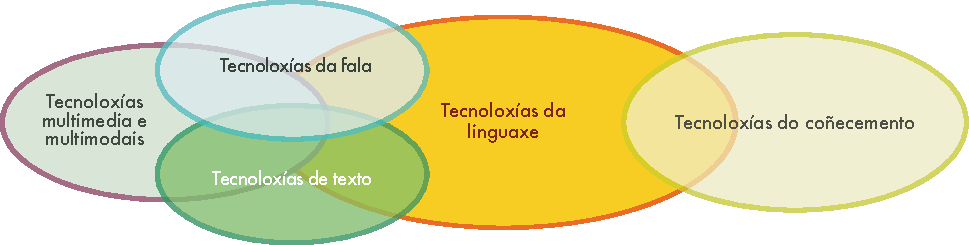
\includegraphics[width=\textwidth]{../_media/galician/language_technologies}
  \caption{***HELPLanguage technologies***FHELP}
  \label{fig:ltincontext_ca}
  \colorrule{grey3}{\textwidth}{1.5pt}
\end{figure*}


Les tecnologies del llenguatge són una àrea establerta de recerca amb un conjunt ampli de literatura introductòria. El lector interessat pot consultar les referències següents: \cite{jurafsky-martin01, manning-schuetze1, lt-world1, lt-survey1}.

Abans de discutir les àrees d'aplicació descrites, descriurem breument l'arquitectura d'un sistema de tecnologies del llenguatge típic.
***FHELP

\subsection[As arquitecturas das aplicacións na tecnoloxías lingüísticas]{As arquitecturas das \newline aplicacións na tecnoloxías lingüísticas}

    As aplicacións informáticas habituais para o tratamento da linguaxe consisten en varios compoñentes que reflicten diversos aspectos da linguaxe e da tarefa que levan a cabo. A Figura 2 presenta unha arquitectura moi simplificada que pode atoparse nun sistema de procesamento de textos. Os tres primeiros módulos tratan a estrutura e o significado do texto de entrada:

\begin{itemize}
      \item Procesamento previo: limpar os datos, eliminar formato, detectar a lingua do texto de entrada, etc.
      \item Análise gramatical: atopar o verbo e os seus obxectos, modificadores, etc.; detectar a estrutura da oración.
      \item Análise semántica: desambiguación (cal dos significados de \textit{gato} é o axeitado no contexto dado?), resolución de anáforas e expresións referenciais como \textit{ela}, o \textit{coche}, etc.; representación do significado da oración de xeito que se poida facer unha lectura automática.
\end{itemize}


    Os módulos de tarefas específicas levan a cabo diferentes operacións, tales como o resumo automático dun texto de entrada, consultas de bases de datos, e moitas outras. Abaixo, mostraremos as áreas principais de aplicación e destacaremos os seus módulos principais. Novamente, as arquitecturas das aplicacións aparecen moi simplificadas para mostrar a complexidade das aplicacións da tecnoloxía lingüística (TL) dun xeito comprensible para o público xeral. As ferramentas e recursos máis importantes aparecen \underline{subliñados no texto} e tamén se poden atopar na táboa ao final do capítulo. As seccións que tratan das principais áreas de aplicación tamén conteñen un resumo do mercado activo nos campos respectivos para o galego.

\begin{figure*}[b]
  \colorrule{grey3}{\textwidth}{1.5pt}
  \center
  \vspace{-5mm} 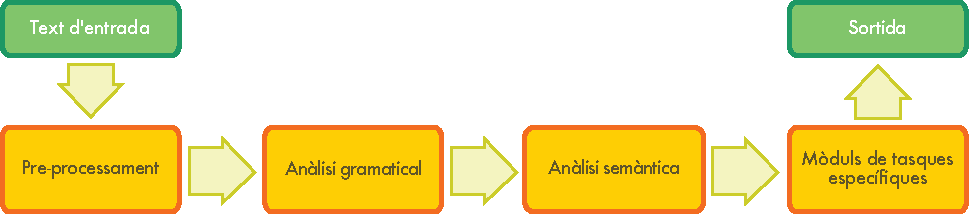
\includegraphics[width=\textwidth]{../_media/catalan/text_processing_app_architecture}
  \caption{Arquitectura típica d'una aplicació de processament de text}
  \label{fig:textprocessingarch_ca}
  \colorrule{grey3}{\textwidth}{1.5pt}
\end{figure*}

Tras facer unha introdución sobre as áreas principais de aplicación, faremos un pequeno repaso da situación na investigación aplicada á tecnoloxía lingüística e á educación, concluíndo cun resumo dos programas de investigación pasados e actuais. Ao final desta sección ofreceremos a opinión dos expertos sobre a situación das principais ferramentas e recursos da tecnoloxía lingüística no tocante a varios aspectos, como a súa dispoñibilidade, madurez ou calidade. Esta táboa proporciona unha boa visión de conxunto sobre a situación da TL para o galego.

\subsection{Principais áreas de aplicación} 

 As seccións que tratan das principais áreas de aplicación tamén conteñen un resumo do mercado activo nos campos respectivos para o galego. As ferramentas e recursos máis importantes aparecen \uline{subliñados no texto} e tamén se poden atopar na táboa ao final do capítulo.

\subsubsection{A corrección lingüística}

   Calquera persoa que empregue unha ferramenta de procesamento de textos, como Microsoft Word, atoparase coa opción de \textbf{corrección ortográfica}, que indica os erros de ortografía e propón as súas correccións. Corenta anos despois do primeiro programa de corrección ortográfica deseñado por Ralph Gorin, hoxe en día os correctores lingüísticos non só comparan a lista de palabras extraídas cun dicionario de palabras correctamente escritas, senón que estes son cada vez máis sofisticados.

Ademais dos algoritmos que dependen do idioma para o tratamento da \uline{morfoloxía} (por exemplo, a formación do plural), algúns son agora capaces de recoñecer erros relacionados coa \uline{sintaxe}, tales como a omisión do verbo ou un verbo que non estea acorde co seu suxeito en persoa e número (por exemplo, “Ela*\uline{escriben} unha carta”). 

Para corrixir automaticamente estes erros, non é suficiente facer unha comprobación de cada palabra no dicionario, xa que todas as palabras da primeira frase son correctas de forma illada. Isto ou ben require a formulación de \uline{normas gramaticais} específicas para cada lingua (é dicir, un alto grao de experiencia e traballo manual), ou o uso dun \uline{modelo lingüístico} estatístico. Estes modelos calculan a probabilidade de que se dea unha palabra nun contexto específico (é dicir, as palabras anteriores e as seguintes). 

 Per exemple, llibre anglès és una seqüència de paraules molt més probable que no pas llibre anglesa. Un model estadístic es pot obtenir automàticament a partir d’una gran quantitat de dades lingüístiques correctes (és a dir, un corpus). Fins al dia d’avui, aquests mètodes s’han desenvolupat i avaluat principalment en anglès. Malauradament, és difícil transferir-los directament al català, que té una inflexió més rica i un ordre sintàctic de les paraules més flexible.

\begin{figure*}[htb]
  \colorrule{grey3}{\textwidth}{1.5pt}
  \vspace{-9mm}
  \center
  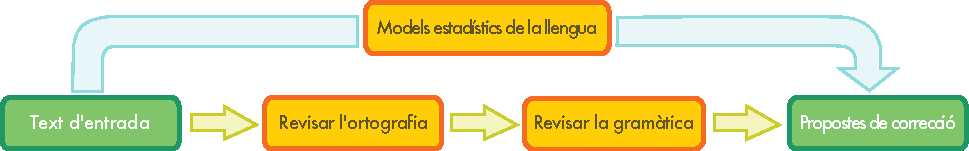
\includegraphics[width=\textwidth]{../_media/catalan/language_checking}
  \caption{Corrector lingüístic (a dalt: estadístic, a baix: basat en regles)}
  \label{fig:langcheckingaarch_ca}
  \colorrule{grey3}{\textwidth}{1.5pt}
\end{figure*}

L’ús d’eines de correcció automàtica no es limita als processadors de textos; també es poden utilitzar com a sistemes de suport per a la creació d’escrits. Degut a l’augment constant de productes tecnològics, la quantitat de documentació tècnica ha crescut ràpidament durant les últimes dècades. Per evitar possibles queixes dels clients per problemes o danys derivats d’una mala comprensió de les instruccions, les empreses han començat a posar més atenció en la qualitat de la documentació tècnica. Els avenços en el processament del llenguatge natural han permès desenvolupar programes de suport que ofereixen ajuda als autors de la documentació i els faciliten la utilització d’un vocabulari i unes estructures d’oracions consistents amb unes determinades regles i restriccions terminològiques (corporatives).

\boxtext{L’ús d’eines de correcció automàtica no es limita als processadors de textos; també es poden utilitzar per a la creació d’escrits}

Només algunes empreses i proveïdors de serveis ofereixen productes en català en aquesta àrea. Enciclopèdia Catalana, Maxigrammar i Inèdit han creat i comercialitzat productes que inclouen la revisió ortogràfica i gramatical per al català, així com eines de revisió adaptades a diversos dominis i estils. Softcatalà i Barcelona Media també han desenvolupat algunes eines lingüístiques que s’ofereixen a la comunitat com a aplicacions web. Una nova versió de “\textit{El corrector}” s’ha desenvolupat i comercialitzat recentment per a Ipod i Ipad. 

A part dels correctors ortogràfics i els programes de suport per a la creació de textos, la revisió dels diferents aspectes lingüístics també és important en l’àmbit dels programes d’ajuda per a l’aprenentatge de llengües, i s’aplica en la correcció automàtica de les cerques enviades als motors de cerca d’Internet (per exemple, en el ‘Volíeu dir:’ de Google). 

\subsubsection{Cerques a la web}

  A busca na web, en intranets, ou en bibliotecas dixitais é probablemente a tecnoloxía lingüística máis empregada hoxe en día á vez que é a menos desenvolvida. O motor de busca Google, que se creou no ano 1998, emprégase hoxe en día para o 80\% das buscas que se realizan en todo o mundo. \cite{CAT-Nota22}. 

Ata o de agora, non houbo cambios significativos con respecto á primeira versión no referente á súa interface de busca nin ao xeito de presentar os resultados obtidos. Na versión actual, Google ofrece unha corrección gramatical para as palabras escritas incorrectamente, mesmo para a versión en galego, e, no ano 2009, incorporáronse posibilidades de busca semántica básica ao seu conxunto de algoritmos\cite{CAT-Nota23}, que melloran a precisión da busca mediante unha análise do significado dos termos da consulta dentro dun contexto. O caso do éxito de Google demostra que, dispoñendo dunha grande cantidade de datos, e con técnicas eficientes para a indexación destes datos, un método baseado principalmente en estatísticas pode producir resultados satisfactorios. 

Non obstante, cando hai unha solicitude de información máis complexa, é fundamental integrar un coñecemento lingüístico máis profundo. Nos laboratorios de investigación, os experimentos levados a cabo empregando tesouros e recursos lingüísticos ontolóxicos como \textit{WordNet} amosaron melloras ao permitir a posibilidade de atopar unha páxina baseándose en sinónimos dos termos empregados na busca, ou mesmo en termos non relacionados directamente. Novamente, estes avances esixen uns recursos lingüísticos específicos. O Centro Ramón Piñeiro para a Investigación en Humanidades\cite{GAL-Nota24} elaborou un \textit{WordNet} para o galego. O \textit{WordNet} galego chámase GALWORDNET.

La propera generació de motors de cerca haurà d’incloure una tecnologia del llenguatge molt més sofisticada. Si els termes d’una consulta consisteixen en una pregunta o un altre tipus de frase, en comptes d’una simple llista de paraules clau, per proporcionar respostes adequades es requereix una \textbf{anàlisi sintàctica} i semàntica de la consulta, a més  a més de la capacitat de crear un índex que permeti trobar ràpidament els documents rellevants per a la resposta. Per exemple, en el cas que un usuari introdueixi la consulta: ‘Dóna’m una llista de totes les empreses que han estat comprades per altres empreses durant els últims cinc anys’. Per proporcionar una resposta satisfactòria, és necessari aplicar una anàlisi sintàctica per tal d’analitzar l’estructura gramatical de l’oració i poder determinar que el que l’usuari desitja és saber quines empreses han estat comprades per altres, i no quines empreses han comprat altres empreses. A més a més, cal processar  l’expressió ‘durant els últims cinc anys’ per determinar el període al qual fa referència la consulta. 

\begin{figure*}[htb]
  \colorrule{grey3}{\textwidth}{1.5pt}
  \vspace{-9mm}
  \center
  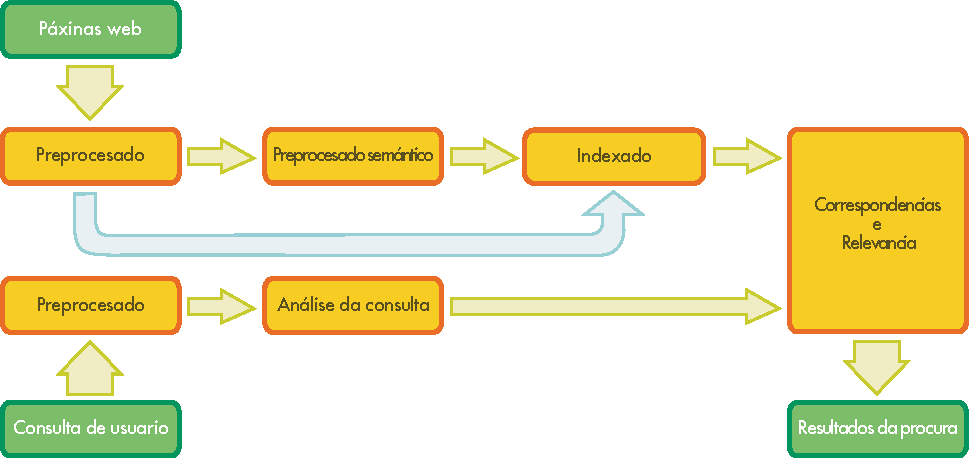
\includegraphics[width=\textwidth]{../_media/galician/web_search_architecture}
  \vspace{-5mm}
  \caption{Cercador web}
  \label{fig:websearcharch_ca}
  \colorrule{grey3}{\textwidth}{1.5pt}
\end{figure*}

Finalmente, a solicitude procesada contrástase cunha grande cantidade de datos non estruturados para atopar a información ou as informacións que o usuario está a solicitar. Este proceso coñécese habitualmente como \uline{recuperación da información}, e implica a busca e a clasificación de documentos relevantes. Ademais, á hora de xerar un listado de compañías, tamén necesitamos extraer a información que fai referencia ao nome dunha compañía dentro dunha cadea de palabras concreta situada nun documento. Este tipo de información está dispoñible grazas aos chamados \uline{recoñecedores de nomes de entidades.} 

Unha tarefa aínda máis difícil é intentar facer coincidir unha busca con documentos escritos noutro idioma. Para a \uline{recuperación de información plurilingüe}, temos que traducir automaticamente a consulta a todas as posibles linguas fonte e volver a pasar a información recuperada á lingua meta. A crecente porcentaxe de datos dispoñibles en formatos non textuais enfoca a demanda cara a servizos que permiten a \uline{recuperación de información multimedia} (é dicir, a busca de información en imaxes, audio e vídeo). Para os arquivos de audio e vídeo, introdúcese un módulo de \uline{recoñecemento do discurso}, que converte o contido do discurso en texto ou nunha representación fonética, e pode facer coincidir coa consulta realizada polo usuario.

Non nos consta que exista tecnoloxía lingüística en compañías dedicadas á busca plurilingüe e á recuperación de información, tanto na Internet como en sistemas de información internos, para o galego. 

  
\subsubsection{A interacción da fala}

  A tecnoloxía de interacción da fala é a base para a creación de interfaces que permiten ao usuario interactuar con máquinas empregando a lingua falada no canto de, por exemplo, un teclado, un rato ou unha pantalla gráfica. Hoxe en día, estas interfaces de usuario baseadas en voz empréganas habitualmente as empresas para proporcionar aos seus clientes, empregados, ou socios, servizos parcialmente ou totalmente automatizados por vía telefónica. 

Os sectores empresariais que dependen en gran medida das interfaces de usuario baseadas en voz son: a banca, a loxística, o transporte público e as telecomunicacións. Outros usos da tecnoloxía de interacción da fala son as interfaces de certos aparellos, como os sistemas de navegación integrados nos auto-móbiles, ou o emprego da lingua falada como alternativa ás modalidades de entrada e saída de información nas interfaces gráficas de usuario, como por exemplo os \textit{smartphones.}


\begin{figure*}[htb]
  \colorrule{grey3}{\textwidth}{1.5pt}
  \vspace{-9mm}
  \center  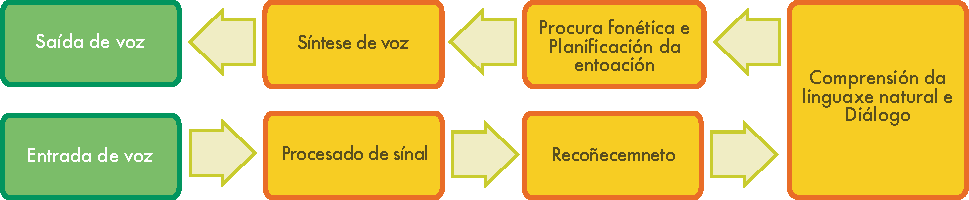
\includegraphics[width=\textwidth]{../_media/galician/simple_speech-based_dialogue_architecture}
  \center
  \caption{***HELPSpeech-based dialogue system***FHELP}
  \label{fig:dialoguearch_ca}
  \colorrule{grey3}{\textwidth}{1.5pt}
\end{figure*}

En esencia, a interacción da fala consta das seguintes catro tecnoloxías: 

    \begin{itemize}
      \item O \uline{recoñecemento automático da fala } (RAF) é o responsable de determinar que palabras foron emitidas tendo en conta a secuencia de sons pronunciados por un usuario.
      \item A \uline{análise sintáctica } e a \uline{interpretación semántica } ocúpanse de analizar a estrutura sintáctica da locución do usuario e da súa posterior interpretación en función da finalidade do sistema respectivo.
      \item A \uline{xestión do diálogo} é necesaria para determinar, pola parte do sistema coa que interactúa o usuario, que acción debe levarse a cabo tendo en conta o \textit{input} do usuario e a funcionalidade do sistema.
      \item A tecnoloxía de  \uline{síntese de diálogo }(texto a voz, TAV) emprégase para transformar as palabras que se emitiron nesa locución en sons que xerarán como resultado unha información de saída para o usuario.  

    \end{itemize}
 
  Un dos maiores retos é que o sistema de RAF recoñeza as palabras pronunciadas por un usuario do xeito máis preciso posible. Isto require ou ben unha restrición da variedade de posibles pronuncias do usuario, para así contar cun conxunto limitado de palabras clave, ou a creación manual de \uline{modelos de linguaxe} que cubran unha grande variedade de pronuncias de usuarios da linguaxe natural. Mentres que o anterior dá como resultado un uso bastante ríxido e inflexible dunha interface de usuario baseada en voz, e posiblemente provoque unha mala aceptación por parte do usuario, a creación, optimización e mantemento de modelos de linguaxe chegan a aumentar os custos considerablemente. Non obstante, as interfaces de usuario baseadas en voz que empregan modelos de linguaxe e que inicialmente permiten que o usuario exprese con flexibilidade as súas intencións (como, por exemplo, nun saúdo como "En que podo axudarlle") amosan tanto un maior grao de automatización como unha maior aceptación por parte do usuario e, polo tanto, poden considerarse vantaxosas mesmo cun enfoque de \textit{diálogo dirixido }  menos flexible.

***HELP\boxtext{Speech interaction is the basis for interfaces that allow a user to interact with spoken language.}***FHELP

No que respecta á saída de información das interfaces de usuario baseadas en voz, as empresan a miúdo adoitan empregar fórmulas previamente gravadas por locutores profesionais (a ser posibles corporativos). Para as locucións estáticas, nas que a redacción non depende do contexto particular de uso, ou dos datos persoais do usuario determinado, isto dará lugar a unha experiencia de usuario satisfactoria. Non obstante, canto máis dinámico sexa o contido que a locución deba ter en conta, a experiencia de usuario sufrirá máis dunha mala prosodia como resultado da concatenación de arquivos de audio individuais. Pola contra, os sistemas actuais de texto a voz demostran ser superiores, a pesar de que se poden mellorar, no referente á naturalidade prosódica das locucións dinámicas. 

Con respecto ao mercado das tecnoloxías de interacción da fala, a última década caracterizouse por unha forte estandarización das interfaces entre os diferentes compoñentes tecnolóxicos, así como polas normas para a creación de aparatos de software particulares para unha determinada aplicación. Tamén existiu unha forte consolidación de mercado nos últimos dez anos, especialmente nos campos do RAF e o TAV. Neste caso, os mercados nacionais dos países do G20 (é dicir, países economicamente fortes cunha poboación considerable) están dominados por menos de 5 reprodutores en todo o mundo, dos cales \textit{Nuance e Loquendo} destacan en Europa, así como para o galego (\textit{Loqueando}); non obstante, algunhas compañías locais máis pequenas están comezando a facer competencia, tales como Verbio \cite{GAL-Nota25} , que é unha versión da Universitat Politècnica de Catalunya e que ten a súa propia tecnoloxía da fala, ou a galega 2Mares \cite{GAL-Nota26}.

En relación á tecnoloxía e ás destrezas de coñecemento da xestión do diálogo, os mercados están fortemente dominados por reprodutores nacionais, que a miúdo se tratan de PEMEs.
A maioría das compañías no mercado do TAV español (algunhas ofrecen galego) son fundamentalmente desenvolvedoras de aplicacións. Os principais reprodutores no mercado español son: Indsys \cite{GAL-Nota27} (Sistemas de diálogo intelixente), Fonetic \cite{GAL-Nota28}, Ydilo \cite{GAL-Nota29}, NaturalVoz \cite{GAL-Nota30}, e 2Mares.

Pero máis aló do estado actual da tecnoloxía, xurdirán importantes cambios debido ao hábito, cada vez máis profuso, de empregar os teléfonos intelixentes (\uline{smartphones}) como unha nova plataforma para xestionar as relacións cos clientes (ademais doutros canais como o teléfono, internet e o correo electrónico). Esta tendencia tamén afectará ao uso da tecnoloxía para a interacción da fala. Por unha banda, diminuirá a largo prazo a demanda de interfaces de usuario baseadas en telefonía. Por outra banda, o emprego da lingua falada cobrará unha importancia considerable nos \uline{smartphones} como modalidade de entrada de información fácil de empregar polos usuarios. Esta tendencia tamén está reforzada pola mellora perceptible de precisión no recoñecemento independente da voz do locutor nos servizos de ditado de discurso que xa se ofrecen como servizos centralizados para os usuarios de \uline{smartphones}. Dada esta "externalización" da tarefa de recoñecemento á infraestrutura das aplicacións, o emprego específico nas aplicacións de tecnoloxías lingüísticas básicas adquirirá probablemente máis importancia que na actualidade. 

\subsubsection{A tradución automática}

  A idea de empregar ordenadores dixitais para a tradución de linguas naturais foi desenvolvida no ano 1946 por A. D. Booth e, na década dos 50, foi acompañada dun financiamento importante para a investigación nesta área, que comezou novamente na década dos 80. Non obstante, a \uline{Tradución Automática} (TA) aínda non consigue cumprir as grandes expectativas que se esperaban nos seus inicios. 

   

\boxtext{No seu nivel básico, a TA simplemente substitúe palabras nunha lingua natural por palabras noutra.}

\begin{figure*}[htb]
  \colorrule{grey3}{\textwidth}{1.5pt}
  \vspace{-21mm}
  \center
  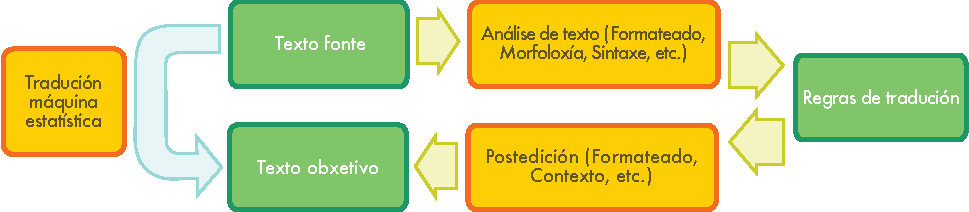
\includegraphics[width=\textwidth]{../_media/galician/machine_translation}
  \vspace{-2mm}
  \caption{Traducció automàtica (a l'esquerra: estadística, a la dreta: basat en regles)}
  \label{fig:mtarch_ca}
  \colorrule{grey3}{\textwidth}{1.5pt}
\end{figure*}

No seu nivel básico, a TA simplemente substitúe palabras nunha lingua natural por palabras noutra. Isto pode resultar útil en disciplinas que posúen unha linguaxe moi restrinxida e con fórmulas establecidas, tales como os informes meteorolóxicos. Non obstante, para que exista unha boa tradución dos textos menos estandarizados, as unidades textuais máis grandes (frases, oracións, ou mesmo pasaxes completas) teñen que coincidir coas súas unidades homólogas máis próximas na lingua meta. Neste caso, a principal dificultade reside no feito de que a linguaxe humana é ambigua, e presenta retos a varios niveis, como por exemplo a \uline{desambiguación do sentido da palabra} a nivel léxico ("Gato" pode significar animal ou aparello mecánico), ou a vinculación de frases preposicionais a nivel sintáctico como en:

\hspace{10pt}O policía observou ao home co telescopio.\\
\hspace{10pt}\textit{[The policeman observed the man with the telescope.]}\\
\hspace{10pt}O policía observou ao home co revólver.\\
\hspace{10pt}\textit{[The policeman observed the man with the revolver.]}

Unha das maneiras para abordar esta tarefa está baseada en regras lingüísticas. Para traducións entre linguas moi relacionadas, unha tradución directa pode resultar viable en casos como o exemplo presentado anteriormente. Non obstante, a miúdo os sistemas baseados en regras (ou baseados no coñecemento) analizan o texto de entrada e crean unha representación simbólica intermediaria, a partir da cal se crea o texto na lingua meta. O éxito destes métodos depende en boa medida da dispoñibilidade de \uline{lexicóns} extensos que contan con información morfolóxica, sintáctica e semántica, así como de grandes conxuntos de regras \uline{gramaticais} coidadosamente deseñadas por lingüistas especializados.

Comezando a finais da década de 1980, e nunha situación na que a informática ía avanzando e se volvía menos cara, empezou a mostrarse cada máis interese nos modelos estatísticos de TA. Os parámetros destes modelos estatísticos derívanse da análise de \uline{corpus} textuais bilingües, como o corpus paralelo Europarl, que contén as actas do Parlamento Europeo en 11 linguas europeas. Cunha cantidade de datos suficiente, a TA estatística funciona bastante ben á hora de obter un significado aproximado dun texto nunha lingua estranxeira. Non obstante, a diferenza dos sistemas baseados no coñecemento, a TA estatística (ou baseada en bases de datos) a miúdo obtén un resultado gramaticalmente incorrecto. Por outra banda, ademais de que grazas a ela requírese menos esforzo humano para realizar unha escritura gramaticalmente correcta, a TA baseada en datos tamén inclúe particularidades da linguaxe que non se inclúen nos sistemas baseados no coñecemento, como por exemplo as expresións idiomáticas. 

Xa que os puntos fortes e febles da TA baseada no coñecemento e da TA baseada en datos son complementarios, hoxe en día os investigadores buscan enfoques híbridos que combinen as metodoloxías de ambas as dúas. Isto pode levarse a cabo de diferentes maneiras. Unha delas é empregar tanto os sistemas baseados en coñecemento como os sistemas baseados en datos e facer que un módulo de selección elixa o mellor resultado para cada oración. Non obstante, no caso das oracións máis longas, non existe un resultado perfecto. Unha solución mellor sería combinar as mellores partes de cada oración extraídas de múltiples resultados, o cal pode resultar bastante complexo, xa que as partes correspondentes obtidas de múltiples alternativas non sempre son obvias e necesitan ser aliñadas. 

Degut a la particular situació oficial de bilingüisme existent a les diferents regions d’Espanya i a la similitud entre el català i el castellà, els sistemes de traducció automàtica entre aquestes dues llengües funcionen de forma bastant satisfactòria. Inicialment, alguns dels principals sistemes que es van desenvolupar van ser el METAL (Siemens) i l’ATLAS (Fujitsu). Aquests projectes van tenir lloc a Barcelona durant els anys 90. Al cap d’un temps, les gran empreses que els van impulsar van apartar-se’n, i els projectes van passar a mans de diferents \textit{spin-off}: una empresa local, INCYTA, així com GMS i Lucy Software, la qual és actualment el proveïdor principal de sistemes de traducció en català, van passar a fer-se càrrec de METAL. A més a més, el sistema de traducció entre el català i el castellà que va comprar la Generalitat de Catalunya va passar a ser un servei web públic l’any 2005, mentre que Google va començar a oferir el seu propi sistema l’any 2007.

Altres empreses, com T6 Estàndard Lingüístic i AutomaticTrans, també han desenvolupat sistemes de traducció automàtica. El sistema desenvolupat per AutomaticTrans té el seu origen en la producció d’un diari bilingüe, El Periódico. Actualment hi ha tres diaris disponibles en català i castellà que utilitzen traducció automàtica; els altres dos són El Segre i La Vanguardia. 

La Generalitat Valenciana va promoure la creació del SALT, un sistema de traducció automàtica específic per al valencià. Més recentment, la Universitat Politècnica de València ha tret una versió de SiShiTra, un sistema híbrid. El sistema de codi obert OpenTrad també ofereix una versió en valencià. 

La traducció entre el català i el castellà va ser l’origen de l’Apertium, un sistema de codi obert desenvolupat pel grup Transducens \cite{CAT-transducens} de la Universitat d’Alacant \cite{CAT-UnivAlacant}. L’Apertium és el primer sistema del món basat en tecnologia de traducció automàtica en codi obert, i la seva explotació comercial la duen a terme principalment Prompsit Language Engineering i OpenTrad Consortium. 

La majoria d’aquests sistemes estan basats en regles. Tot i que s’estan fent esforços importants, tant a nivell nacional com internacional, per millorar els sistemes estadístics i híbrids, aquests mètodes encara no proporcionen les mateixes prestacions en aplicacions comercials que en l’àmbit de la recerca. 

Donada una bona adaptació en termes de terminologia específica per l’usuari i una bona integració en el ritme de treball, l’ús de la traducció automàtica pot incrementar la productivitat significativament. Així, des de començaments del segle XXI, el principal usuari d’aquests sistemes en català és l’administració pública, inclosos alguns departaments del govern com el de justícia.

Es considera que la qualitat dels sistemes de traducció encara té un gran marge de millora. Alguns dels principals reptes són aconseguir adaptar els recursos lingüístics a un determinat domini i la integració en processos de treballs existents amb bases terminològiques i memòries de traducció.

A més a més, la majoria de corpus paraŀlels existents són entre el català i el castellà, de manera que en la majoria de traductors per al català, el castellà és la llengua pivot.

\begin{figure*}[tb]
  \centering
  \setlength{\tabcolsep}{0.17em}
  \small
  \begin{tabular}{>{\columncolor{corange1}}cccccccccccccccccccccccc}
    & \multicolumn{22}{>{\columncolor{corange1}}c}{Target language -- \textcolor{grey1}{Target language}}\\\addlinespace[{-.009cm}]
    \rowcolor{corange1}  & EN & BG & DE & CS & DA & EL & ES & ET & FI & FR & HU & IT & LT & LV & MT & NL & PL & PT & RO & SK & SL & SV\\
    EN & -- & \textcolor{blue}{40.5} & \textcolor{blue}{46.8} & \textcolor{green2}{52.6} & \textcolor{green2}{50.0} & \textcolor{blue}{41.0} & \textcolor{green2}{55.2} & \textcolor{purple}{34.8} & \textcolor{purple}{38.6} & \textcolor{green2}{50.1} & \textcolor{purple}{37.2} & \textcolor{green2}{50.4} & \textcolor{purple}{39.6} & \textcolor{blue}{43.4} & \textcolor{purple}{39.8} & \textcolor{green2}{52.3} & \textcolor{blue}{49.2} & \textcolor{green2}{55.0} & \textcolor{blue}{49.0} & \textcolor{blue}{44.7} & \textcolor{green2}{50.7} & \textcolor{green2}{52.0}\\
    BG & \textcolor{green}{61.3} & -- & \textcolor{purple}{38.7} & \textcolor{purple}{39.4} & \textcolor{purple}{39.6} & \textcolor{purple}{34.5} & \textcolor{blue}{46.9} & \textcolor{red3}{25.5} & \textcolor{red3}{26.7} & \textcolor{blue}{42.4} & \textcolor{red3}{22.0} & \textcolor{blue}{43.5} & \textcolor{red3}{29.3} & \textcolor{red3}{29.1} & \textcolor{red3}{25.9} & \textcolor{blue}{44.9} & \textcolor{purple}{35.1} & \textcolor{blue}{45.9} & \textcolor{purple}{36.8} & \textcolor{purple}{34.1} & \textcolor{purple}{34.1} & \textcolor{purple}{39.9}\\
    DE & \textcolor{green2}{53.6} & \textcolor{red3}{26.3} & -- & \textcolor{purple}{35.4} & \textcolor{blue}{43.1} & \textcolor{purple}{32.8} & \textcolor{blue}{47.1} & \textcolor{red3}{26.7} & \textcolor{red3}{29.5} & \textcolor{purple}{39.4} & \textcolor{red3}{27.6} & \textcolor{blue}{42.7} & \textcolor{red3}{27.6} & \textcolor{purple}{30.3} & \textcolor{red2}{19.8} & \textcolor{green2}{50.2} & \textcolor{purple}{30.2} & \textcolor{blue}{44.1} & \textcolor{purple}{30.7} & \textcolor{red3}{29.4} & \textcolor{purple}{31.4} & \textcolor{blue}{41.2}\\
    CS & \textcolor{green2}{58.4} & \textcolor{purple}{32.0} & \textcolor{blue}{42.6} & -- & \textcolor{blue}{43.6} & \textcolor{purple}{34.6} & \textcolor{blue}{48.9} & \textcolor{purple}{30.7} & \textcolor{purple}{30.5} & \textcolor{blue}{41.6} & \textcolor{red3}{27.4} & \textcolor{blue}{44.3} & \textcolor{purple}{34.5} & \textcolor{purple}{35.8} & \textcolor{red3}{26.3} & \textcolor{blue}{46.5} & \textcolor{purple}{39.2} & \textcolor{blue}{45.7} & \textcolor{purple}{36.5} & \textcolor{blue}{43.6} & \textcolor{blue}{41.3} & \textcolor{blue}{42.9}\\
    DA & \textcolor{green2}{57.6} & \textcolor{red3}{28.7} & \textcolor{blue}{44.1} & \textcolor{purple}{35.7} & -- & \textcolor{purple}{34.3} & \textcolor{blue}{47.5} & \textcolor{red3}{27.8} & \textcolor{purple}{31.6} & \textcolor{blue}{41.3} & \textcolor{red3}{24.2} & \textcolor{blue}{43.8} & \textcolor{red3}{29.7} & \textcolor{purple}{32.9} & \textcolor{red3}{21.1} & \textcolor{blue}{48.5} & \textcolor{purple}{34.3} & \textcolor{blue}{45.4} & \textcolor{purple}{33.9} & \textcolor{purple}{33.0} & \textcolor{purple}{36.2} & \textcolor{blue}{47.2}\\
    EL & \textcolor{green2}{59.5} & \textcolor{purple}{32.4} & \textcolor{blue}{43.1} & \textcolor{purple}{37.7} & \textcolor{blue}{44.5} & -- & \textcolor{green2}{54.0} & \textcolor{red3}{26.5} & \textcolor{red3}{29.0} & \textcolor{blue}{48.3} & \textcolor{red3}{23.7} & \textcolor{blue}{49.6} & \textcolor{red3}{29.0} & \textcolor{purple}{32.6} & \textcolor{red3}{23.8} & \textcolor{blue}{48.9} & \textcolor{purple}{34.2} & \textcolor{green2}{52.5} & \textcolor{purple}{37.2} & \textcolor{purple}{33.1} & \textcolor{purple}{36.3} & \textcolor{blue}{43.3}\\
    ES & \textcolor{green}{60.0} & \textcolor{purple}{31.1} & \textcolor{blue}{42.7} & \textcolor{purple}{37.5} & \textcolor{blue}{44.4} & \textcolor{purple}{39.4} & -- & \textcolor{red3}{25.4} & \textcolor{red3}{28.5} & \textcolor{green2}{51.3} & \textcolor{red3}{24.0} & \textcolor{green2}{51.7} & \textcolor{red3}{26.8} & \textcolor{purple}{30.5} & \textcolor{red3}{24.6} & \textcolor{blue}{48.8} & \textcolor{purple}{33.9} & \textcolor{green2}{57.3} & \textcolor{purple}{38.1} & \textcolor{purple}{31.7} & \textcolor{purple}{33.9} & \textcolor{blue}{43.7}\\
    ET & \textcolor{green2}{52.0} & \textcolor{red3}{24.6} & \textcolor{purple}{37.3} & \textcolor{purple}{35.2} & \textcolor{purple}{37.8} & \textcolor{red3}{28.2} & \textcolor{blue}{40.4} & -- & \textcolor{purple}{37.7} & \textcolor{purple}{33.4} & \textcolor{purple}{30.9} & \textcolor{purple}{37.0} & \textcolor{purple}{35.0} & \textcolor{purple}{36.9} & \textcolor{red3}{20.5} & \textcolor{blue}{41.3} & \textcolor{purple}{32.0} & \textcolor{purple}{37.8} & \textcolor{red3}{28.0} & \textcolor{purple}{30.6} & \textcolor{purple}{32.9} & \textcolor{purple}{37.3}\\
    FI & \textcolor{blue}{49.3} & \textcolor{red3}{23.2} & \textcolor{purple}{36.0} & \textcolor{purple}{32.0} & \textcolor{purple}{37.9} & \textcolor{red3}{27.2} & \textcolor{purple}{39.7} & \textcolor{purple}{34.9} & -- & \textcolor{red3}{29.5} & \textcolor{red3}{27.2} & \textcolor{purple}{36.6} & \textcolor{purple}{30.5} & \textcolor{purple}{32.5} & \textcolor{red2}{19.4} & \textcolor{blue}{40.6} & \textcolor{red3}{28.8} & \textcolor{purple}{37.5} & \textcolor{red3}{26.5} & \textcolor{red3}{27.3} & \textcolor{red3}{28.2} & \textcolor{purple}{37.6}\\
    FR & \textcolor{green}{64.0} & \textcolor{purple}{34.5} & \textcolor{blue}{45.1} & \textcolor{purple}{39.5} & \textcolor{blue}{47.4} & \textcolor{blue}{42.8} & \textcolor{green}{60.9} & \textcolor{red3}{26.7} & \textcolor{purple}{30.0} & -- & \textcolor{red3}{25.5} & \textcolor{green2}{56.1} & \textcolor{red3}{28.3} & \textcolor{purple}{31.9} & \textcolor{red3}{25.3} & \textcolor{green2}{51.6} & \textcolor{purple}{35.7} & \textcolor{green}{61.0} & \textcolor{blue}{43.8} & \textcolor{purple}{33.1} & \textcolor{purple}{35.6} & \textcolor{blue}{45.8}\\
    HU & \textcolor{blue}{48.0} & \textcolor{red3}{24.7} & \textcolor{purple}{34.3} & \textcolor{purple}{30.0} & \textcolor{purple}{33.0} & \textcolor{red3}{25.5} & \textcolor{purple}{34.1} & \textcolor{red3}{29.6} & \textcolor{red3}{29.4} & \textcolor{purple}{30.7} & -- & \textcolor{purple}{33.5} & \textcolor{red3}{29.6} & \textcolor{purple}{31.9} & \textcolor{red2}{18.1} & \textcolor{purple}{36.1} & \textcolor{red3}{29.8} & \textcolor{purple}{34.2} & \textcolor{red3}{25.7} & \textcolor{red3}{25.6} & \textcolor{red3}{28.2} & \textcolor{purple}{30.5}\\
    IT & \textcolor{green}{61.0} & \textcolor{purple}{32.1} & \textcolor{blue}{44.3} & \textcolor{purple}{38.9} & \textcolor{blue}{45.8} & \textcolor{blue}{40.6} & \textcolor{red3}{26.9} & \textcolor{red3}{25.0} & \textcolor{red3}{29.7} & \textcolor{green2}{52.7} & \textcolor{red3}{24.2} & -- & \textcolor{red3}{29.4} & \textcolor{purple}{32.6} & \textcolor{red3}{24.6} & \textcolor{green2}{50.5} & \textcolor{purple}{35.2} & \textcolor{green2}{56.5} & \textcolor{purple}{39.3} & \textcolor{purple}{32.5} & \textcolor{purple}{34.7} & \textcolor{blue}{44.3}\\
    LT & \textcolor{green2}{51.8} & \textcolor{red3}{27.6} & \textcolor{purple}{33.9} & \textcolor{purple}{37.0} & \textcolor{purple}{36.8} & \textcolor{red3}{26.5} & \textcolor{red3}{21.1} & \textcolor{purple}{34.2} & \textcolor{purple}{32.0} & \textcolor{purple}{34.4} & \textcolor{red3}{28.5} & \textcolor{purple}{36.8} & -- & \textcolor{blue}{40.1} & \textcolor{red3}{22.2} & \textcolor{purple}{38.1} & \textcolor{purple}{31.6} & \textcolor{purple}{31.6} & \textcolor{red3}{29.3} & \textcolor{purple}{31.8} & \textcolor{purple}{35.3} & \textcolor{purple}{35.3}\\
    LV & \textcolor{green2}{54.0} & \textcolor{red3}{29.1} & \textcolor{purple}{35.0} & \textcolor{purple}{37.8} & \textcolor{purple}{38.5} & \textcolor{red3}{29.7} & \textcolor{red2}{8.0} & \textcolor{purple}{34.2} & \textcolor{purple}{32.4} & \textcolor{purple}{35.6} & \textcolor{red3}{29.3} & \textcolor{purple}{38.9} & \textcolor{purple}{38.4} & -- & \textcolor{red3}{23.3} & \textcolor{blue}{41.5} & \textcolor{purple}{34.4} & \textcolor{purple}{39.6} & \textcolor{purple}{31.0} & \textcolor{purple}{33.3} & \textcolor{purple}{37.1} & \textcolor{purple}{38.0}\\
    MT & \textcolor{green}{72.1} & \textcolor{purple}{32.2} & \textcolor{purple}{37.2} & \textcolor{purple}{37.9} & \textcolor{purple}{38.9} & \textcolor{purple}{33.7} & \textcolor{blue}{48.7} & \textcolor{red3}{26.9} & \textcolor{red3}{25.8} & \textcolor{blue}{42.4} & \textcolor{red3}{22.4} & \textcolor{blue}{43.7} & \textcolor{purple}{30.2} & \textcolor{purple}{33.2} & -- & \textcolor{blue}{44.0} & \textcolor{purple}{37.1} & \textcolor{blue}{45.9} & \textcolor{purple}{38.9} & \textcolor{purple}{35.8} & \textcolor{blue}{40.0} & \textcolor{blue}{41.6}\\
    NL & \textcolor{green2}{56.9} & \textcolor{red3}{29.3} & \textcolor{blue}{46.9} & \textcolor{purple}{37.0} & \textcolor{blue}{45.4} & \textcolor{purple}{35.3} & \textcolor{blue}{49.7} & \textcolor{red3}{27.5} & \textcolor{red3}{29.8} & \textcolor{blue}{43.4} & \textcolor{red3}{25.3} & \textcolor{blue}{44.5} & \textcolor{red3}{28.6} & \textcolor{purple}{31.7} & \textcolor{red3}{22.0} & -- & \textcolor{purple}{32.0} & \textcolor{blue}{47.7} & \textcolor{purple}{33.0} & \textcolor{purple}{30.1} & \textcolor{purple}{34.6} & \textcolor{blue}{43.6}\\
    PL & \textcolor{green}{60.8} & \textcolor{purple}{31.5} & \textcolor{blue}{40.2} & \textcolor{blue}{44.2} & \textcolor{blue}{42.1} & \textcolor{purple}{34.2} & \textcolor{blue}{46.2} & \textcolor{red3}{29.2} & \textcolor{red3}{29.0} & \textcolor{blue}{40.0} & \textcolor{red3}{24.5} & \textcolor{blue}{43.2} & \textcolor{purple}{33.2} & \textcolor{purple}{35.6} & \textcolor{red3}{27.9} & \textcolor{blue}{44.8} & -- & \textcolor{blue}{44.1} & \textcolor{purple}{38.2} & \textcolor{purple}{38.2} & \textcolor{purple}{39.8} & \textcolor{blue}{42.1}\\
    PT & \textcolor{green}{60.7} & \textcolor{purple}{31.4} & \textcolor{blue}{42.9} & \textcolor{purple}{38.4} & \textcolor{blue}{42.8} & \textcolor{blue}{40.2} & \textcolor{green}{60.7} & \textcolor{red3}{26.4} & \textcolor{red3}{29.2} & \textcolor{green2}{53.2} & \textcolor{red3}{23.8} & \textcolor{green2}{52.8} & \textcolor{red3}{28.0} & \textcolor{purple}{31.5} & \textcolor{red3}{24.8} & \textcolor{blue}{49.3} & \textcolor{purple}{34.5} & -- & \textcolor{purple}{39.4} & \textcolor{purple}{32.1} & \textcolor{purple}{34.4} & \textcolor{blue}{43.9}\\
    RO & \textcolor{green}{60.8} & \textcolor{purple}{33.1} & \textcolor{purple}{38.5} & \textcolor{purple}{37.8} & \textcolor{blue}{40.3} & \textcolor{purple}{35.6} & \textcolor{green2}{50.4} & \textcolor{red3}{24.6} & \textcolor{red3}{26.2} & \textcolor{blue}{46.5} & \textcolor{red3}{25.0} & \textcolor{blue}{44.8} & \textcolor{red3}{28.4} & \textcolor{red3}{29.9} & \textcolor{red3}{28.7} & \textcolor{blue}{43.0} & \textcolor{purple}{35.8} & \textcolor{blue}{48.5} & -- & \textcolor{purple}{31.5} & \textcolor{purple}{35.1} & \textcolor{purple}{39.4}\\
    SK & \textcolor{green}{60.8} & \textcolor{purple}{32.6} & \textcolor{purple}{39.4} & \textcolor{blue}{48.1} & \textcolor{blue}{41.0} & \textcolor{purple}{33.3} & \textcolor{blue}{46.2} & \textcolor{red3}{29.8} & \textcolor{red3}{28.4} & \textcolor{purple}{39.4} & \textcolor{red3}{27.4} & \textcolor{blue}{41.8} & \textcolor{purple}{33.8} & \textcolor{purple}{36.7} & \textcolor{red3}{28.5} & \textcolor{blue}{44.4} & \textcolor{purple}{39.0} & \textcolor{blue}{43.3} & \textcolor{purple}{35.3} & -- & \textcolor{blue}{42.6} & \textcolor{blue}{41.8}\\
    SL & \textcolor{green}{61.0} & \textcolor{purple}{33.1} & \textcolor{purple}{37.9} & \textcolor{blue}{43.5} & \textcolor{blue}{42.6} & \textcolor{purple}{34.0} & \textcolor{blue}{47.0} & \textcolor{purple}{31.1} & \textcolor{red3}{28.8} & \textcolor{purple}{38.2} & \textcolor{red3}{25.7} & \textcolor{blue}{42.3} & \textcolor{purple}{34.6} & \textcolor{purple}{37.3} & \textcolor{purple}{30.0} & \textcolor{blue}{45.9} & \textcolor{purple}{38.2} & \textcolor{blue}{44.1} & \textcolor{purple}{35.8} & \textcolor{purple}{38.9} & -- & \textcolor{blue}{42.7}\\
    SV & \textcolor{green2}{58.5} & \textcolor{red3}{26.9} & \textcolor{blue}{41.0} & \textcolor{purple}{35.6} & \textcolor{blue}{46.6} & \textcolor{purple}{33.3} & \textcolor{blue}{46.6} & \textcolor{red3}{27.4} & \textcolor{purple}{30.9} & \textcolor{purple}{38.9} & \textcolor{red3}{22.7} & \textcolor{blue}{42.0} & \textcolor{red3}{28.2} & \textcolor{purple}{31.0} & \textcolor{red3}{23.7} & \textcolor{blue}{45.6} & \textcolor{purple}{32.2} & \textcolor{blue}{44.2} & \textcolor{purple}{32.7} & \textcolor{purple}{31.3} & \textcolor{purple}{33.5} & --\\
    \end{tabular}
  \caption{Traducció automàtica entre 22 llengües europees -- \textcolor{grey1}{Machine translation between 22 EU-languages \cite{euro1}}}
  \label{fig:euromatrix_en}
\end{figure*}

Les campanyes avaluadores ajuden a comparar la qualitat dels sistemes de traducció automàtica, les seves aproximacions i l'estat dels sistemes per diferents parelles d'idiomes. La figura~\ref{fig:euromatrix_en} (p.~\pageref{fig:euromatrix_en}), que es va preparar durant el projecte Euromatrix+, mostra les actuacions per parelles obtingudes per 22 dels 23 idiomes de la Unió Europea (L'irlandès no va comparar-se). Els resultats s'ordenen d'acord a una puntuació BLEU, que indica més altes puntuacions per millors traduccions \cite{bleu1}. Un traductor humà aconseguiria normalment al voltant de 80 punts. Els millors resultats (en verd i blau) van ser aconseguits per idiomes que es beneficien d'un esforç de recerca considerable en programes coordinats i en l'existència de molts còrpora paral·lels (p. ex: anglès, francès, holandès, espanyol i alemany). Els idiomes amb els resultats més pobres es mostren en vermell. A aquests els manquen els esforços de desenvolupament mencionats o són estructuralment molt diferents dels altres idiomes (p. ex: hongarès, maltès, finès)

\subsection{***HELP Other Application Areas ***FHELP}

   A creación de aplicacións de tecnoloxía lingüística implica unha serie de subtarefas que non sempre se desenvolven no plano da interacción co usuario, senón que proporcionan importantes prestacións de servizo "baixo a carcasa" do sistema. Polo tanto, estas aplicacións constitúen asuntos importantes de investigación, e chegaron a converterse en subdisciplinas individuais no ámbito académico dentro da Lingüística Informática. 

\uline{A resposta a preguntas} converteuse nunha área de investigación, para a cal se construíron \uline{corpus} anotados e se empezaron a levar a cabo competicións científicas. A idea é pasar da busca baseada en palabras clave (para a cal o motor responde cunha colección enteira de documentos potencialmente relevantes) a unha situación na que o usuario realiza unha pregunta concreta e o sistema proporciona unha soa resposta: "A que idade puxo Neil Armstrong pé na lúa?" - "38". Mentres que isto está obviamente relacionado coa área principal da busca na web, hoxe en día a resposta a preguntas é principalmente un termo xenérico para as preguntas de investigación tales como que tipos de preguntas deberían distinguirse e como deberían tratarse, como poden analizarse e compararse un conxunto de documentos que potencialmente conteñen a resposta (ofrecen respostas contraditorias?), e como pode extraerse de xeito fiable unha información específica -a resposta- dun documento, sen ignorar excesivamente o contexto. 

Isto está, á vez, relacionado coa tarefa de \uline{extracción de información} (EI), unha área que se volveu moi popular e influente na época do "cambio estatístico" na Lingüística Computacional a principios da década dos 90. A EI ten como obxectivo identificar extractos de información específicos dentro dun tipo específico de documentos; un exemplo disto podería ser o descubrimento dos axentes clave na absorción de empresas tal como informan os artigos xornalísticos. Outra hipótese na que se traballou é os informes sobre atentados terroristas, onde o problema reside en estruturar o texto seguindo un modelo que especifique o autor do crime, o obxectivo, a hora e localización do atentado, e os resultados do mesmo. Cubrir modelos sobre dominios específicos é a principal característica da EI, que por esta razón é outro exemplo dunha tecnoloxía "non visible" que constitúe unha área de investigación ben delimitada pero que, a efectos prácticos, necesita estar integrada dentro dun contorno de aplicacións axeitado. 

\boxtext{***HELP Las aplicaciones de las tecnologias del lenguaje proporcionan servicios yi funciones importantes para el sistema poco perceptibles por el usuario final.***FHELP}

Existen dúas áreas "dubidosas" que ás veces desempeñan o papel de aplicacións independentes, e outras veces a de compoñentes de apoio "baixo a carcasa" do sistema, que son o \uline{resumo do texto} e a \uline{produción do texto}. O resumo, obviamente, refírese á tarefa de converter un texto longo en curto, e ofrécese, por exemplo, como función dentro de MS Word. Funciona en gran medida sobre unha base estatística, identificando primeiro as palabras "importantes" nun texto (é dicir, por exemplo, palabras que son moi frecuentes neste texto, pero notablemente menos frecuentes no uso xeral da lingua) e, a continuación, determinando as oracións que conteñen moitas palabras importantes. Logo, estas oracións márcanse no documento, ou extráense del, e cóllense para compoñer o resumo. Neste caso, que é sen dúbida o máis común, o resumo é igual á extracción da oración: o texto redúcese a un subconxunto das súas oracións. Todos os resumidores comerciais fan uso desta idea. Un enfoque alternativo, ao que se dedicaron algunhas investigacións, é o de sintetizar novas oracións, é dicir, construír un resumo de oracións que non aparecen necesariamente nesa forma no texto orixinal. Isto require unha certa comprensión máis profunda do texto e, polo tanto, resulta moito menos robusto. En definitiva, un xerador de texto na maioría dos casos non é unha aplicación independente senón que está integrado nun contorno de software máis grande, como no sistema de información clínica onde se recollen, almacenan e procesan os datos dos pacientes, e a xeración de informes é só unha de entre moitas funcións.


\boxtext{Para el gallego, como para la mayoría de las lenguas,  la investigación de las tecnologías del lenguaje se encuentra mucho menos desarrollada que para el inglés.}

No caso do galego, a situación nestas áreas de investigación está moito menos desenvolvida que no caso do inglés, onde, desde a década de 1990, a resposta a preguntas, a extracción de información e a síntese foron obxecto de numerosas competicións, principalmente as organizadas por DARPA/NIST en Estados Unidos. Estas melloraron notablemente a tecnoloxía punta, pero sempre se fixo fincapé no idioma inglés; algunhas competicións engadiron pistas plurilingües, pero nunca se empregou a lingua galega. Como consecuencia, apenas existen corpus anotados ou outros recursos para estas tarefas. Os sistemas de resumo, cando empregan métodos puramente estatísticos, adoitan ser en boa medida independentes da lingua, e polo tanto están dispoñibles algúns prototipos de investigación. Para a xeración de texto, os compoñentes reutilizables tradicionalmente estaban limitados aos módulos de desenvolvemento da superficie (as "gramáticas de xeración"); unha vez máis, atopamos que a maioría do software dispoñible é para o inglés. 

Ademais dos sistemas experimentais desenvolvidos polos grupos de investigación, non existen PEMEs que ofrezan este tipo de servizos. Desde o ano 2000 ata hoxe, o goberno español vén apoiando, dentro do Plan Nacional de Investigación e Tecnoloxía, varios proxectos na área das tecnoloxías da fala plurilingües: TEHAM, AVIVAVOZ, e BUCEADOR. O seu principal propósito era mellorar a calidade do recoñecemento da fala, da tradución da fala e da síntese de texto a voz en todas as linguas oficiais de España: éuscaro, galego, catalán e español.

\subsection{A tecnoloxía lingüística na educación}

   A tecnoloxía lingüística é un eido sumamente interdisciplinario, no que participan expertos lingüistas, informáticos, matemáticos, filósofos, psicolingüistas e neurólogos, entre outros. Como consecuencia, a actual formación básica dun lingüista informático en España debe levarse a cabo no marco dun título en Filoloxía ou Lingüística, que inclúa á Lingüística Informática como materia troncal, ou nas facultades de Informática. Entre as universidades que ofrecen a primeira opción están: A Universitat de Barcelona, a Universitat Pompeu Fabra, a Universitat Oberta de Catalunya e a Universidade de Vigo. Por outra banda, as principais facultades de informática que ofrecen como materia a Lingüística Informática son: A Universidade Politécnica de Madrid, a Universidade Carlos III, a Universidade Autónoma de Madrid, a Universitat d’Alacant, a Universidade Nacional de Educación a Distancia, e a Euskal Herriko Unibertsitatea. Outros casos, como a Universidade Complutense, combina ambos os dous.

Os cursos de posgrao ofrecen unha formación profesional máis específica. Existen varios programas de doutoramento que ofrecen másteres ou materias relacionadas co procesamento da fala e da linguaxe. Algunhas universidades, como a Universidade Politécnica de Cataluña, tamén participan no Máster Europeo en Linguaxe e Fala, avalado pola ELSNET (Rede de Excelencia Europea en Tecnoloxías Lingüísticas). Existen varios másteres en diversas universidades, a nivel nacional ou a nivel europeo; por exemplo, a Universitat Autònoma de Barcelona ofrece o Máster Internacional en Procesamento de Linguaxe Natural e Tecnoloxías Lingüísticas, en colaboración con universidades estranxeiras. Noutros másteres ou cursos de doutoramento tamén se imparten módulos sobre tecnoloxías lingüísticas, especialmente en Tradución (por exemplo, nas universidades Autónoma de Barcelona, Alacante, Castellón, Politécnica de Valencia e Granada).

Existen máis de 30 grupos de investigación en España repartidos nas diferentes universidades, que traballan no recoñecemento da fala, o procesamento de linguaxe natural, a tradución de texto a texto, e a síntese da fala. A Sociedade Española para o Procesamento da Linguaxe Natural (SEPLN) é unha organización sen ánimo de lucro con máis de 300 membros, tanto do ámbito académico como da industria, que foi creada en 1984 co propósito de promover e difundir as actividades relacionadas coa docencia, a investigación e o desenvolvemento do PLN, tanto a nivel nacional como internacional. A SEPLN organiza seminarios, simposios e conferencias, e promove a colaboración con institucións nacionais e internacionais.

Tamén organiza unha conferencia anual, á que cada ano asisten máis investigadores que traballan sobre o PLN, tanto de España como do estranxeiro. A asociación tamén edita unha revista periódica e mantén un servidor web con información sobre cuestións relacionadas co procesamento de linguaxe natural, así como un foro aberto para os membros.

A Rede Temática en Tecnoloxías da Fala (RTTF) española \cite{GAL-Nota34} é un foro común onde os investigadores (actualmente máis de 250) en tecnoloxías da fala xuntan esforzos e comparten experiencias para:
	\begin{itemize}
		\item Promover a investigación nas tecnoloxías da fala para atraer os investigadores novos neste campo mediante a formación, os intercambios de estudantes, as bolsas e os premios.
		\item Atraer inversións para a investigación empresarial mediante o desenvolvemento de aplicacións innovadoras que ofrezan novas oportunidades de negocio. 
		\item Progresar no establecemento de alianzas e na integración dos membros da rede para manter o liderado de España na investigación do español, e impulsar tamén os idiomas cooficiais como o catalán, o éuscaro e o galego.
	\end{itemize}

Dende o ano 2000, a RTTF vén promovendo as "Xornadas en Tecnoloxía da Fala" bianuais. Este seminario ten como obxectivo converterse nun punto de encontro para presentar e discutir os resultados da investigación sobre a fala e as tecnoloxías lingüísticas nos idiomas ibéricos. Tamén busca promover a colaboración entre a industria e as universidades. Lévanse a cabo unha ampla variedade de actividades, como presentacións de relatorios técnicos, conferencias maxistrais, presentación de informes dos proxectos e actividades dos laboratorios, demostracións, e presentacións recentes de teses de doutoramento.

\subsection{Programas de tecnoloxía lingüística}

   Os Ministerios de Educación e Ciencia e Innovación españois apoian a investigación no eido das tecnoloxías da información a través de programas nacionais de investigación. Estes programas impulsaron numerosos proxectos de investigación e colaboración con centros de investigación e empresas internacionais. A base do desenvolvemento da tecnoloxía e das aplicacións comerciais para o procesamento automatizado da lingua española creouse en parte como resultado destes proxectos.
	
O Centro para o Desenvolvemento da Tecnoloxía Industrial (CDTI) é unha entidade pública española dependente do Ministerio de Ciencia e Innovación, cuxo obxectivo é axudar ás empresas españolas a mellorar o seu nivel tecnolóxico. O CDTI avalía e financia proxectos de I+D a través de programas como CENIT e AVANZA.

O programa CENIT (Consorcio Estratéxico Nacional para a Investigación Tecnolóxica) busca estimular a cooperación en I+D entre o sector privado, as universidades, as organizacións e centros públicos de investigación, os parques de ciencia e tecnoloxía e os centros tecnolóxicos, así como impulsar a cooperación público-privada en I+D. Os proxectos do CENIT duran polo menos catro anos e teñen un presuposto mínimo de 5 millóns de euros ao ano, durante os cales recibirán un financiamento mínimo do 50\% do sector privado. Polo menos o 50\% do financiamento público destinarase aos centros públicos de investigación ou aos centros tecnolóxicos. A tecnoloxía da información e da comunicación é unha das áreas de prioridade do programa. Os proxectos levados a cabo nesta área inclúen ás veces investigación sobre tecnoloxías lingüísticas. 

O obxectivo do plan AVANZ@ é achegar a sociedade da información aos cidadáns ordinarios, así como aos sectores público e privado. A promoción do uso das tecnoloxías TIC terá importantes repercusións en todos os sectores en xeral dentro de España e, polo tanto, no seu estado de innovación. Os obxectivos do plan inclúen incrementar a porcentaxe de empresas que utilizan o comercio electrónico, promover o uso da factura electrónica, ampliar o sector público electrónico mediante a posta en funcionamento dunha tarxeta de identidade electrónica e de rexistro electrónico, alcanzar un índice dun ordenador con acceso á Internet por cada dous alumnos nas escolas, e duplicar o número de fogares con acceso á Internet. Unha das súas prioridades é facilitar o uso de novas tecnoloxías aos anciáns e ás persoas minusválidas como medio ideal para a integración social, evitar a marxinación e mellorar a súa calidade de vida. As ferramentas da tecnoloxía lingüística fáciles de usar ofrecen a principal solución para satisfacer este obxectivo, por exemplo, proporcionando unha síntese da fala para as persoas invidentes.

A Xunta de Galicia apoia a investigación a través do Plan Galego de Investigación, Desenvolvemento e Innovación Tecnolóxica (PGIDIT). A tecnoloxía lingüística non é unha área de prioridade pero, ao longo dos 
anos, os grupos de investigación das universidades e algunhas empresas conseguiron bolsas para levar a cabo investigacións e desenvolvementos na TL.

\subsection{Dispoñibilidade de ferramentas e recursos para o idioma galego}

   A seguinte táboa proporciona unha visión xeral da situación actual do apoio das tecnoloxías lingüísticas para o idioma galego. A valoración dos recursos e ferramentas existentes está baseada en estudos estimados levados a cabo por expertos, que empregaron os seguintes criterios (comprendidos entre 0 e 6). 
 
\begin{figure*}[htb]
  \centering
\begin{tabular}{>{\columncolor{orange1}}p{.33\linewidth}@{\hspace*{6mm}}c@{\hspace*{6mm}}c@{\hspace*{6mm}}c@{\hspace*{6mm}}c@{\hspace*{6mm}}c@{\hspace*{6mm}}c@{\hspace*{6mm}}c}
\rowcolor{orange1}
 \cellcolor{white}&
 \begin{sideways}\makecell[l]{Quantitat}\end{sideways} &
 \begin{sideways}\makecell[l]{\makecell[l]{Disponibilitat} }\end{sideways} &
 \begin{sideways}\makecell[l]{Qualitat}\end{sideways} &
 \begin{sideways}\makecell[l]{Cobertura}\end{sideways} &
 \begin{sideways}\makecell[l]{Maduresa}\end{sideways} &
 \begin{sideways}\makecell[l]{Sostenibilitat}\end{sideways} &
 \begin{sideways}\makecell[l]{Adaptabilitat}\end{sideways} \\ \addlinespace

\multicolumn{8}{>{\columncolor{orange2}}l}{\textcolor{black}{Tecnologies del llenguatge: eines, tecnologies i aplicacions}} \\ \addlinespace

Reconeixement de la parla	&3&3&3&3&3&3&2 \\ \addlinespace
Síntesi de veu &4&2&4&4&5&4&2\\ \addlinespace
Anàlisi gramatical &3&2.5&4&4&4&2.5&2.5\\ \addlinespace
Anàlisi semàntic &1&1&2&1&1&1&1\\ \addlinespace
Generació de text &1&2&3&1&3&3&1\\ \addlinespace
Traducció automàtica &3&3&2&3&4&1&2\\ \addlinespace

\multicolumn{8}{>{\columncolor{orange2}}l}{\textcolor{black}{Recursos lingüístics: recursos, dades, bases de coneixement}} \\ \addlinespace

Corpora textuals &3&2.5&3.5&3&3&2.5&2.5\\ \addlinespace
Corpora orals &3&5&3&2&3&3&2\\ \addlinespace
Corpora paraŀlels &2&1&2&2&2&1&1\\ \addlinespace
Recursos lèxics &2.5&2&3&2.5&3&3&2.5\\ \addlinespace
Gramàtiques &2&3&2&2&2&2&2\\
\end{tabular}
 \caption{Estat del suport a les tecnologies del llenguatge pel Català}
 \label{tab:lrlttable}
\end{figure*}

A situación do galego no que respecta ao apoio das tecnoloxías lingüísticas dá lugar a un optimismo cauto. Grazas ao apoio dalgúns proxectos de investigación levados a cabo anteriormente, hoxe en día existen en España un panorama de investigación e unha industria da tecnoloxía lingüística emerxentes, que desenvolven produtos e servizos para o idioma galego. A industria está conformada por PEMEs, a maioría das cales xurdiron a raíz dun proxecto ou un grupo de investigación. 

No caso do galego, existen varias tecnoloxías e recursos, pero moitas menos que para o inglés. Así e todo, mesmo no caso do inglés e doutras linguas principais, o apoio da tecnoloxía lingüística hoxe en día aínda está lonxe de ofrecer o soporte necesario que precisa unha verdadeira sociedade plurilingüe do coñecemento.

Nesta serie de libros brancos, levouse a cabo un primeiro esforzo de avaliar a situación xeral de moitas linguas europeas no tocante ao apoio da tecnoloxía lingüística dun xeito que permitise a comparación e identificación exhaustiva de carencias e necesidades.

Para o galego, os principais resultados en relación ás tecnoloxías e recursos son os seguintes:
	\begin{itemize}
		\item O procesamento da fala actualmente parece estar máis desenvolvido có procesamento do texto escrito. As tecnoloxías de acceso á información avanzada aínda se atopan nos seus comezos e, para o caso do galego en particular, apenas existen.
		\item Canto máis coñecemento lingüístico e semántico inclúe unha ferramenta, máis carencias aparecen (véxase, por exemplo, a recuperación de información contra a semántica textual) e son necesarios máis esforzos para dar apoio ao procesamento lingüístico exhaustivo. 
		\item A investigación tivo éxito á hora de deseñar software de alta calidade, pero moitos dos recursos carecen de estandarización, é dicir, mesmo se existen, non sempre teñen a sostibilidade necesaria; precísanse iniciativas e programas concertados para estandarizar os datos e os formatos de intercambio.
		\item	Para o galego existe un amplo corpus textual de referencia (cunha mestura equilibrada de diversos xéneros), así como outros corpus especializados, mais estes non son facilmente accesibles nin baratos.
		\item Aínda que existen algúns corpus específicos de alta calidade, non se dispón dun corpus extenso anotado sintacticamente.
		\item Existen moi poucos corpus anotados con información sintáctica, semántica ou discursiva e, polo tanto, a situación empeora cando se precisa información lingüística e semántica máis profunda.
		\item O procesamento da fala está actualmente máis desenvolvida ca o PLN para os textos escritos.
		\item Existen corpus paralelos entre o galego e o español, e estes foron empregados para o desenvolvemento de sistemas de tradución automática. Non obstante, hai unha ausencia de corpus paralelos entre o galego e outras linguas.
		\item Os datos multimedia constitúen tamén unha enorme carencia.
 	\end{itemize}
É por isto que queda claro que é preciso centrar máis esforzos na creación de recursos para o galego, así como na investigación, innovación e desenvolvemento. A necesidade de grandes cantidades de datos e a enorme complexidade dos sistemas informáticos que incorporan tecnoloxías lingüísticas tamén obrigan a desenvolver novas infraestruturas para o intercambio e a cooperación.

\subsection{Comparación entre linguas}
   O estado actual de apoio ás tecnoloxías da linguaxe varía considerablemente dunha comunidade lingüística a outra. Para comparar a situación entre as linguas, esta sección presentará unha avaliación baseada en dúas áreas concretas de aplicación (a tradución automática e o procesamento de voz) e unha tecnoloxía subxacente (análise textual), así como nos recursos básicos necesarios para construír aplicacións para as tecnoloxías da lingua.


Figura 1: Agrupacións de idiomas para o Procesamento da Fala

Figura 2: Agrupacións de idiomas para a Tradución Automática

Descrición dos grupos (para o Procesamento da Fala e a Tradución Automática)
	\begin{itemize}
	\item Grupo 1 (excelente soporte ás tecnoloxías da lingua): Existencia de tecnoloxías de excelente calidade e prestacións. Poden ser empregadas en practicamente todas as aplicacións relevantes.
	\item Grupo 2 (moi bo soporte): Existencia de tecnoloxías de boa calidade e prestacións. Poden ser empregadas en diversas aplicacións. 
	\item Grupo 3 (bo soporte): Existencia de tecnoloxías dunha calidade e prestacións razoables. O seu uso está limitado a algunhas aplicacións ou dominios.
	\item Grupo 4 (soporte medio): Existencia de prototipos de investigación, primeiras aplicacións comerciais ou servizos gratuítos de calidade e prestacións diferentes.
	\item Grupo 5 (pouco soporte ou case inexistente): Tecnoloxías en fase de deseño ou prototipos rudimentarios cunha calidade e prestacións moi limitadas.
	\end{itemize}

Figura 3: Agrupacións de idiomas para a Análise Textual

Figura 4: Agrupacións de idiomas para os Recursos

Descrición dos grupos (por Análise Textual e Recursos)
	\begin{itemize}
	\item Grupo 1 (excelente soporte): Existencia de tecnoloxías e recursos de uso xeral que cobren practicamente todos os fenómenos lingüísticos (vocabulario, compostos, gramática, metáforas, etc.) dunha lingua.
	\item Grupo 2 (moi bo soporte): Existencia de tecnoloxías e recursos que se empregan nunha ampla variedade de aplicacións e cobren os fenómenos lingüísticos máis importantes.
	\item Grupo 3 (bo soporte): Existencia de tecnoloxías e recursos que cobren unha cantidade razoable dos fenómenos lingüísticos e que se empregan en aplicacións que adoitan ser de dominios específicos.
	\item Grupo 4 (soporte medio): Existencia de prototipos de investigación e recursos que varían en calidade e cobertura.
	\item Grupo 5 (pouco soporte ou case inexistente): Prototipos en fase de deseño ou rudimentarios (calidade e cobertura moi limitadas, sistemas de xoguete).
	\end{itemize}

As táboas anteriores mostran que, grazas a programas para o financiamento das tecnoloxías da linguaxe dos gobernos español e galego nas últimas décadas, o galego está ao nivel da maioría das outras linguas europeas. É semellante a outras linguas cun número similar de falantes, como Finlandia ou Noruega, a pesar de que estes son idiomas oficiais de estados da Unión Europea. Non obstante, os recursos e ferramentas para as tecnoloxías da linguaxe no caso do galego aínda non chegan á cobertura e calidade de recursos e ferramentas comparables no caso da lingua española, que se sitúa nunha boa posición en case todas as áreas das tecnoloxías da lingua, a pesar de que aínda hai moitas lagoas nos recursos en español en canto ás aplicacións de alta calidade.

Para o procesamento da fala, as tecnoloxías actuais conseguen integrarse con éxito nunha serie de aplicacións industriais, como por exemplo os sistemas interactivos activados por voz e sistemas de ditado en dominios restrinxidos. Os sistemas de tradución automática obteñen boas prestacións, especialmente entre os pares de linguas español-galego. Porén, para a construción de aplicacións máis sofisticadas, como por exemplo a tradución automática en amplos dominios e linguas, existe unha clara necesidade de recursos e tecnoloxías que cubran unha gama máis ampla dos aspectos lingüísticos e permitan unha análise semántica en profundidade do texto de entrada. Mediante a mellora da calidade e cobertura destes recursos e tecnoloxías básicas, seremos quen de abrir novas oportunidades para abordar unha ampla gama de áreas de aplicación avanzadas, incluíndo a tradución automática de alta calidade.

L'estat actual del suport a les tecnologies de llenguatge varia considerablement d'una comunitat lingüística a una altra. Per tal de comparar la situació entre llengües, aquesta secció presentarà una avaluació basada en dos exemples d'àrees d'aplicació de les tecnologies del llenguatge (traducció automàtica i processat de la parla) i una tecnologia subjacent (anàlisi de textos), així com recursos bàsics necessaris per construir aplicacions de les tecnologies del llenguatge.
Les llengües es van classificar utilitzant l'escala de cinc punts següent:

\begin{enumerate}
\item Suport exceŀlent
\item Suport bo
\item Suport moderat
\item Suport parcial
\item Suport feble o inexistent
\end{enumerate}

El suport a les tecnologies del llenguatge es va mesurar d'acord amb els criteris següents:

\textbf{Processament de la parla:} Qualitat de les tecnologies de reconeixement de la parla existents, qualitat de les tecnologies de síntesi de veu  existents, cobertura de dominis de la parla, nombre i mida dels corpora de la parla existents, quantitat i varietat de les aplicacions basades en la parla disponible.

\textbf{Traducció automàtica:} Qualitat de les tecnologies de traducció automàtica existents, nombre de parelles de llengues cobertes, cobertura de dominis i fenòmens lingüístics, qualitat i mida dels corpora paraŀlels existents, quantitat i varietat d'aplicacions de traducció automàtica disponibles.

\textbf{Anàlisi del text:} Qualitat i cobertura de les tecnologies d'anàlisi de texts existents (morfologia, sintàxi, semàntiques), cobertura de dominis i fenòmens lingüístics, quantitat i varietat d'aplicacions disponibles, qualitat i mida dels corpora (etiquetats) de text existents, qualitat i cobertura dels recursos lèxics (p. ex: WordNet) i gramàtiques.

\textbf{Recursos:} Qualitat i mida dels corpora de text existents, corpora de la parla i corpora paraŀlels, qualitat i cobertura de recursos lèxics i gramaticals existents.

\begin{figure*}
\small
\centering
\begin{tabular}
{ % defines color for each column.
>{\columncolor{corange5}} p{.17\linewidth}@{\hspace{.027\linewidth}}
>{\columncolor{corange4}}p{.17\linewidth}@{\hspace{.027\linewidth}}
>{\columncolor{corange3}}p{.17\linewidth}@{\hspace{.027\linewidth}}
>{\columncolor{corange2}}p{.17\linewidth}@{\hspace{.027\linewidth}}
>{\columncolor{corange1}}p{.17\linewidth} 
}
\rowcolor{orange1} % redefines color for all columns in row 1
\begin{center}\vspace*{-2mm}\textbf{Excel·lent}\end{center} & 
\begin{center}\vspace*{-2mm}\textbf{Bo}\end{center} & 
\begin{center}\vspace*{-2mm}\textbf{Moderat}\end{center} & 
\begin{center}\vspace*{-2mm}\textbf{Fragmentat}\end{center} & 
\begin{center}\vspace*{-2mm}\textbf{Pobre/Inexistent}\end{center} \\ \addlinespace
% "Pobre/Inexistent" may be changed to "Pobre/No" if "Inexistent" is too long

& \vspace*{0.5mm}
Anglès
& \vspace*{0.5mm}
Alemany \newline   
Espanyol \newline
Finès \newline 
Francès \newline 
Holandès \newline 
Italià \newline  
Portuguès \newline 
Txec \newline 
& \vspace*{0.5mm}
Basc \newline 
Búlgar \newline 
\textbf{Català} \newline 
Danès \newline 
Eslovac \newline 
Eslovè \newline 
Estonià \newline 
Gallec \newline 
Grec \newline  
Hongarès  \newline
Irlandès \newline  
Noruec \newline 
Polonès \newline 
Serbi \newline 
Suec \newline
& \vspace*{0.5mm}
Croat \newline 
Islandès \newline  
Letó \newline 
Lituà \newline 
Maltès \newline 
Romanès\\
\end{tabular}
\caption{Grups de llengües en funció de l’estat actual del processament de la parla}
\label{fig:speech_cluster}
\end{figure*}

\begin{figure*}
\small
\centering
\begin{tabular}
{ % defines color for each column.
>{\columncolor{corange5}} p{.17\linewidth}@{\hspace{.027\linewidth}}
>{\columncolor{corange4}}p{.17\linewidth}@{\hspace{.027\linewidth}}
>{\columncolor{corange3}}p{.17\linewidth}@{\hspace{.027\linewidth}}
>{\columncolor{corange2}}p{.17\linewidth}@{\hspace{.027\linewidth}}
>{\columncolor{corange1}}p{.17\linewidth} 
}
\rowcolor{orange1} % redefines color for all columns in row 1
\begin{center}\vspace*{-2mm}\textbf{Excel·lent}\end{center} & 
\begin{center}\vspace*{-2mm}\textbf{Bo}\end{center} & 
\begin{center}\vspace*{-2mm}\textbf{Moderat}\end{center} & 
\begin{center}\vspace*{-2mm}\textbf{Fragmentat}\end{center} & 
\begin{center}\vspace*{-2mm}\textbf{Pobre/Inexistent}\end{center} \\ \addlinespace
% "Pobre/Inexistent" may be changed to "Pobre/No" if "Inexistent" is too long

& \vspace*{0.5mm} Anglès 
& \vspace*{0.5mm} 
Francès \newline 
Espanyol
& \vspace*{0.5mm}
Alemany \newline 
\textbf{Català} \newline 
Holandès \newline 
Hongarès \newline
Italià \newline 
Polonès \newline 
Romanès \newline 
& \vspace*{0.5mm}
Basc \newline 
Búlgar \newline 
Croat \newline 
Danès \newline 
Eslovac \newline 
Eslovè \newline 
Estonià \newline 
Finès \newline 
Gallec \newline 
Grec \newline 
Irlandès \newline 
Islandès \newline 
Letó \newline 
Lituà \newline 
Maltès \newline 
Noruec \newline 
Portuguès \newline 
Serbi \newline 
Suec \newline 
Txec \newline
\end{tabular}
\caption{Grups de llengües en funció de l’estat actual de la traducció automàtica}
\label{fig:mt_cluster}
\end{figure*}

\begin{figure*}
  \small
  \centering
  \begin{tabular}
{ % defines color for each column.
>{\columncolor{corange5}} p{.17\linewidth}@{\hspace{.027\linewidth}}
>{\columncolor{corange3}}p{.17\linewidth}@{\hspace{.027\linewidth}}
>{\columncolor{corange3}}p{.17\linewidth}@{\hspace{.027\linewidth}}
>{\columncolor{corange2}}p{.17\linewidth}@{\hspace{.027\linewidth}}
>{\columncolor{corange1}}p{.17\linewidth} 
}
\rowcolor{orange1} % redefines color for all columns in row 1
\begin{center}\vspace*{-2mm}\textbf{Excel·lent}\end{center} & 
\begin{center}\vspace*{-2mm}\textbf{Bo}\end{center} & 
\begin{center}\vspace*{-2mm}\textbf{Moderat}\end{center} & 
\begin{center}\vspace*{-2mm}\textbf{Fragmentat}\end{center} & 
\begin{center}\vspace*{-2mm}\textbf{Pobre/Inexistent}\end{center} \\ \addlinespace
% "Pobre/Inexistent" may be changed to "Pobre/No" if "Inexistent" is too long

& \vspace*{0.5mm}Anglès
& \vspace*{0.5mm}
  Alemany \newline 
  Espanyol\newline 
  Francès \newline 
  Holandès \newline 
  Italià 
& \vspace*{0.5mm}
  Basc \newline 
  Búlgar \newline 
  \textbf{Català} \newline 
  Danès \newline 
  Eslovac \newline 
  Eslovè \newline 
  Finès \newline 
  Gallec \newline 
  Grec \newline 
  Hongarès \newline 
  Noruec \newline 
  Polonès \newline 
  Portuguès \newline 
  Romanès \newline 
  Suec \newline 
  Txec \newline 
& \vspace*{0.5mm}
  Croat \newline 
  Estonià \newline 
  Irlandès \newline 
  Islandès \newline 
  Letó \newline 
  Lituà \newline 
  Maltès \newline 
  Serbi \\
  \end{tabular}
\caption{Grups de llengües en funció de l’estat actual dels analitzadors de textos}
\label{fig:text_cluster}
\end{figure*}

\begin{figure*}
  \small
  \centering
\begin{tabular}
{ % defines color for each column.
>{\columncolor{corange5}} p{.17\linewidth}@{\hspace{.027\linewidth}}
>{\columncolor{corange4}}p{.17\linewidth}@{\hspace{.027\linewidth}}
>{\columncolor{corange3}}p{.17\linewidth}@{\hspace{.027\linewidth}}
>{\columncolor{corange2}}p{.17\linewidth}@{\hspace{.027\linewidth}}
>{\columncolor{corange1}}p{.17\linewidth} 
}
\rowcolor{orange1} % redefines color for all columns in row 1
\begin{center}\vspace*{-2mm}\textbf{Excel·lent}\end{center} & 
\begin{center}\vspace*{-2mm}\textbf{Bo}\end{center} & 
\begin{center}\vspace*{-2mm}\textbf{Moderat}\end{center} & 
\begin{center}\vspace*{-2mm}\textbf{Fragmentat}\end{center} & 
\begin{center}\vspace*{-2mm}\textbf{Pobre/Inexistent}\end{center} \\ \addlinespace
% "Pobre/Inexistent" may be changed to "Pobre/No" if "Inexistent" is too long
    
& \vspace*{0.5mm}Anglès
& \vspace*{0.5mm} 
    Alemany \newline 
    Espanyol \newline
    Francès \newline 
    Holandès \newline 
    Hongarès \newline
    Italià \newline
    Polonès \newline
    Suec \newline 
    Txec \newline 
& \vspace*{0.5mm}
    Basc\newline 
    Búlgar\newline 
    \textbf{Català} \newline 
    Croat \newline 
    Danès \newline 
    Eslovac \newline 
    Eslovè \newline
    Estonià \newline 
    Finès \newline 
    Gallec \newline 
    Grec \newline 
    Noruec \newline 
    Portuguès \newline 
    Romanès \newline 
    Serbi \newline 
&  \vspace*{0.5mm}
    Irlandès \newline 
    Islandès \newline 
    Letó \newline 
    Lituà \newline 
    Maltès  \\
  \end{tabular}
  \caption{Grups de llengües en funció de l’estat actual dels recursos }
  \label{fig:resources_cluster}
\end{figure*}

Les taules anteriors mostren que, gràcies als programes per al finançament de les tecnologies del llenguatge dels governs espanyol i català en les últimes dècades, el català està al nivell de la majoria d'altres llengües europees. Es compara bé amb els idiomes amb un nombre similar de parlants, com l'hungarès, el grec i el portuguès (europeu), tot i que aquests són idiomes oficials en països de la UE. No obstant això, els recursos i eines per a les tecnologies del llenguatge en català no arriben encara a la cobertura i qualitat dels recursos i eines comparables per a la llengua espanyola, que està en una bona posició en gairebé totes les àrees de les tecnologies del llenguatge, tot i que encara hi ha molt a millorar en els seus recursos pel que fa a les aplicacions d'alta qualitat.

Per al processament de la parla, la tecnologia actual aconsegueix integrar-se amb èxit en una sèrie d'aplicacions industrials, com ara els sistemes interactius activats per veu i sistemes de dictat en dominis restringits. Els sistemes de traducció automàtica obtenen bones prestacions, especialment entre els parells d'idiomes espanyol-català i català-anglès. No obstant això, per a la construcció d'aplicacions més sofisticades, com ara la traducció automàtica en amplis dominis i llengües, hi ha una clara necessitat d'obtenir recursos i tecnologia que cobreixin una gamma més àmplia dels aspectes lingüístics i que permetin una anàlisi en profunditat semàntica del text d'entrada. Mitjançant la millora de la qualitat i cobertura d'aquests recursos i tecnologia bàsica, serem capaços d'obrir noves oportunitats per abordar una àmplia gamma d'àrees d'aplicació avançades, incloent-hi la traducció automàtica d'alta qualitat.

\subsection{Conclusións}

\emph{Nesta serie de libros brancos fixemos un importante esforzo inicial para avaliar o apoio das tecnoloxías da linguaxe no caso de 30 linguas europeas, e proporcionar unha comparación de alto nivel entre estes idiomas. Ao identificar as carencias, necesidades e deficiencias, a comunidade europea das tecnoloxías da linguaxe e outras partes interesadas poden agora deseñar un programa de investigación e desenvolvemento a grande escala dirixido á construción dunha Europa verdadeiramente plurilingüe e tecnoloxicamente avanzada.}

Xa vimos que existen grandes diferenzas entre as linguas de Europa. Se ben hai software de boa calidade e recursos dispoñibles nalgúns idiomas e áreas de aplicación, noutros (normalmente no caso das linguas “máis pequenas”) teñen importante lagoas. Moitas linguas non contan con tecnoloxías básicas para a análise textual e os recursos esenciais para o desenvolvemento destas tecnoloxías. Outros teñen ferramentas e recursos básicos, pero aínda son incapaces de investir no procesamento semántico; por tanto, aínda teñen que facer un esforzo a grande escala para acadar o ambicioso obxectivo de proporcionar unha tradución automática de alta calidade entre todos os idiomas europeos.

No caso do galego, somos moderadamente optimistas sobre o estado actual do apoio ás tecnoloxías da lingua. En Galicia existe unha comunidade investigadora en tecnoloxías da lingua, que conta co apoio de programas de investigación dos gobernos español e galego. Producíronse e distribuíronse unha serie de recursos e tecnoloxías de última xeración para o galego; non obstante, o alcance destes recursos e a variedade de ferramentas son aínda moi limitados en comparación cos recursos e ferramentas dispoñibles no caso da lingua española (e obviamente para o idioma inglés), e simplemente non son suficientes en calidade e cantidade para desenvolver o tipo de tecnoloxías necesarias que permiten apoiar unha sociedade do coñecemento verdadeiramente plurilingüe.

A industria galega das tecnoloxías da linguaxe dedicada a transformar a investigación en produtos é actualmente moi pequena. A maioría de empresas grandes pararon a súa actividade ou ben reduciron drasticamente os seus esforzos en tecnoloxías da lingua, deixando os idiomas falados por un número reducido de persoas nun segundo plano.

As nosas achegas mostran que a única alternativa é facer un esforzo importante por crear recursos para as tecnoloxías da linguaxe para o galego, e de empregalos para impulsar a investigación, a innovación e o desenvolvemento. A necesidade de grandes cantidades de datos e a extrema complexidade dos sistemas das tecnoloxías da linguaxe fai que sexa crucial desenvolver unha nova infraestrutura e unha organización de investigación máis coherente para estimular un maior intercambio e cooperación.

Tamén existe unha carencia de continuidade no financiamento da investigación e o desenvolvemento. Os programas coordinados a curto prazo tenden a alternarse con períodos de financiamento escaso ou nulo. Ademais, existe unha carencia xeral de coordinación cos programas doutros países da UE e coa Comisión Europea.

Polo tanto podemos concluír que é necesaria unha iniciativa ampla e coordenada que se centre en superar as diferenzas á hora de dispoñer de tecnoloxía lingüística no conxunto das linguas europeas.

A longo prazo, o obxectivo de META-NET é introducir tecnoloxías da linguaxe de alta calidade para todas as linguas co fin de acadar unha unidade política e económica a través da diversidade cultural. A tecnoloxía axudará a eliminar as barreiras existentes e construír pontes entre as linguas europeas. Isto require que todas as partes interesadas, tanto do eido da política, a investigación, as empresas e a sociedade, unan os seus esforzos para o futuro.



\end{multicols}

\cleardoublepage


% --------------------------------------------------------------------------
\ssection[Quant a META-NET]{Quant a META-NET}

\begin{multicols}{2}

   META-NET é unha Rede de Excelencia financiada pola Unión Europea. Actualmente está formada por 47 membros, que representan a 31 países europeos, os cales se enumeran a continuación. META-NET está construíndo a Alianza Tecnolóxica Plurilingüe de Europa (META), unha crecente comunidade de organizacións e profesionais das tecnoloxías lingüísticas en Europa. 

	Figura 5: Países representados en META-NET

META-NET coopera cunha ducia de iniciativas importantes como CLARIN, que está a axudar ás ciencias sociais a establecer o eido das Humanidades Dixitais en Europa. META-NET dedícase a fomentar os fundamentos tecnolóxicos para establecer e manter unha verdadeira sociedade europea da información plurilingüe que

\begin{itemize}

	\item permita a comunicación e cooperación entre as linguas, 
	\item asegure aos usuarios de calquera idioma o acceso á información e ao coñecemento,
	\item ofreza funcionalidades avanzadas de tecnoloxías da información en rede a todos os cidadáns e a un prezo asumible. 
\end{itemize}

META-NET fomenta e promove as tecnoloxías plurilingües para todas as linguas europeas. As tecnoloxías permiten a tradución automática, a produción de contidos, o procesamento da información e a xestión do coñecemento para unha ampla variedade de aplicacións e de disciplinas. A rede pretende mellorar os enfoques actuais para que se poida establecer unha mellor comunicación e cooperación entre linguas. Todos os europeos teñen o mesmo dereito á información e o coñecemento, independentemente da súa lingua. 


\end{multicols}
\cleardoublepage


% --------------------------------------------------------------------------
\ssection[As tres liñas de acción de META-NET]{As tres liñas de acción de META-NET}

\begin{multicols}{2}

  META-NET presentouse o 1 de febreiro de 2010 co obxectivo de avanzar na investigación sobre a tecnoloxía lingüística. A iniciativa apoia unha Europa unida nun único mercado dixital e espazo de información. META-NET vén levando a cabo diversas actividades que promoven os seus obxectivos. META-VISION, META-SHARE e META-RESEARCH son as tres liñas de acción da rede.

Figure6: Tres liñas de acción en META-NET

\textbf{META-VISION} fomenta a construción dunha comunidade dinámica e influínte arredor dunha visión compartida e unha axenda estratéxica de investigación (AEI). O principal enfoque desta actividade é constru-ír unha comunidade dedicada ás tecnoloxías lingüísticas en Europa que sexa coherente e cohesiva, reunindo aos representantes de grupos de interesados sumamente divididos e diversos. Durante o primeiro ano de META-NET, as presentacións no Foro FLaReNet (España), as Xornadas sobre tecnoloxía lingüística (Luxemburgo), JIAMCATT 2010 (Luxemburgo), LREC 2010 (Malta), EAMT 2010 (Francia) e ICT 2010 (Bélxica) centráronse na divulgación. Segundo as previsións iniciais, META-NET xa contactou con máis de 2.500 profesionais no eido das tecnoloxías lingüísticas para compartir con eles os seus obxectivos e visións. META-NET compartiu os resultados iniciais do seu proceso de elaboración dunha visión común no evento META-FORUM 2010, celebrado en Bruxelas, que contou con máis de 250 participantes. Nunha serie de sesións interactivas, os participantes intercambiaron opinións acerca das visións presentadas pola rede. 

\textbf{META-SHARE} crea un portal aberto e distribuído para compartir e intercambiar recursos. A rede \uline{peer-to-peer} de repositorios conterá datos da linguaxe, ferramentas, e servizos web documentados con metadatos de alta calidade e organizados en categorías estandarizadas. Pódese acceder facilmente aos recursos e buscalos de maneira uniforme. Os recursos dispoñibles inclúen materiais gratuítos e de código aberto, así como elementos restrinxidos, dispoñibles no mercado, mediante o seu pago. META-SHARE diríxese aos datos lingüísticos existentes, ferramentas e sistemas informáticos, así como aos produtos novos e emerxentes que se precisan para construír e avaliar novas tecnoloxías, produtos e servizos. A reutilización, combinación, adaptación e remodelación das ferramentas e dos datos lingüísticos xogan un papel crucial. META-SHARE converterase nunha parte fundamental do mercado das tecnoloxías lingüísticas para os desenvolvedores, expertos en localización, investigadores, tradutores e profesionais da linguaxe, tanto de empresas pequenas, como medianas e grandes. META-SHARE aborda o ciclo completo de desenvolvemento da tecnoloxía lingüística, dende a investigación ata os produtos e servizos innovadores. Un aspecto clave desta actividade é establecer META-SHARE como unha parte importante e valiosa dunha infraestrutura europea e global para a comunidade dedicada á TL. 

 \textbf{META-RESEARCH} constrúe pontes cara a campos tecnolóxicos relacionados. Esta actividade busca provocar avances noutros campos e sacar partido da investigación innovadora que poida beneficiar á tecnoloxía lingüística. En concreto, esta actividade pretende dotar de máis semántica á tradución automática (TA), optimizar a división do traballo na TA híbrida, explotar o uso do contexto na tradución automática por ordenador e preparar unha base empírica para a TA. META-RESEARCH traballa con outros campos e disciplinas, como a aprendizaxe automática e a comunidade dedicada á web semántica. META-RESEARCH céntrase na recollida de datos, preparación de conxuntos de datos e organización de recursos lingüísticos para fins de avaliación; elaboración de inventarios de ferramentas e métodos; e organización de obradoiros e eventos de formación para os membros da comunidade. Esta actividade identificou claramente aspectos da TA onde a semántica pode influír nas boas prácticas actuais. Ademais, a actividade creou recomendacións sobre como tratar o problema da integración da información semántica na TA. META-RESEARCH está a finalizar un novo recurso lingüístico para a TA, o corpus anotado para unha mostra de TA híbrida, que proporciona datos para os pares de linguas inglés-alemán, inglés-español e inglés-checo. META-RESEARCH tamén desenvolveu software que compila corpus plurilingües que están ocultos na Internet.
 

\end{multicols}
\cleardoublepage

\vfill

\makeatletter
\@ifundefined{theHsection}{
  \let
}
{
  \renewcommand*{\theHsection}{\thepart.\thesection}
}
\makeatother
\part*{\textcolor{white}{English}}
\setcounter{section}{0}
\setcounter{figure}{0}

\centerline{office@meta-net.eu -- http://www.meta-net.eu}

\addtocontents{toc}{\protect\clearpage\protect}
\addtocontents{toc}{\protect\thispagestyle{empty}\protect}
\addtocontents{toc}{\protect\vspace*{4mm}\protect}
\addtocontents{toc}{\smallskip{\Large\textsf{\centerline{THE CATALAN LANGUAGE IN THE DIGITAL AGE}}\par}}

\cleardoublepage

\selectlanguage{english}


% Start of english part
% --------------------------------------------------------------------------
\ssection[Executive Summary]{Executive Summary}

\begin{multicols}{2}
    
    During the last 60 years, Europe has become a distinct political and economic structure, yet culturally and linguistically it is still very diverse. This means that from Portuguese to Polish and Italian to Icelandic, everyday communication between Europe’s citizens as well as communication in the spheres of business and politics is inevitably confronted by language barriers. The EU’s institutions spend about a billion euros a year on maintaining their policy of multilingualism, i.e., translating texts and interpreting spoken communication. Yet does this have to be such a burden? Modern language technology and linguistic research can make a significant contribution to pulling down these linguistic borders. When combined with intelligent devices and applications, language technology will in the future be able to help Europeans talk easily to each other and do business with each other even if they do not speak a common language. 

    \boxtext{Language technology builds bridges for Europe’s future}

    The European economy takes greater advantage than others from the European single market: In 2010, trade within the EU accounted for 60.3\% of German exports, and trade with other European countries totalled another 10.8\%. But language barriers can bring business to a halt, especially for SMEs who do not have the financial means to reverse the situation. The only (unthinkable) alternative to this kind of multilingual Europe would be to allow a single language to take a dominant position and end up replacing all other languages. 

    One classic way of overcoming the language barrier is to learn foreign languages. Yet without technological support, mastering the 23 official languages of the member states of the European Union and some 60 other European languages is an insurmountable obstacle for the citizens of Europe and its economy, political debate, and scientific progress. 

    The solution is to build key enabling technologies. These will offer European actors tremendous advantages, not only within the common European market but also in trade relations with third countries, especially emerging economies. To achieve this goal and preserve Europe’s cultural and linguistic diversity, it is necessary to first carry out a systematic analysis of the linguistic particularities of all European languages, and the current state of language technology support for them. Language technology solutions will eventually serve as a unique bridge between Europe’s languages. 

    The automated translation and speech processing tools currently available on the market still fall short of this ambitious goal. The dominant actors in the field are primarily privately-owned for-profit enterprises based in Northern America. Already in the late 1970s, the EU realised the profound relevance of language technology as a driver of European unity, and began funding its first research projects, such as EUROTRA. At the same time, national projects were set up that generated valuable results but never led to concerted European action. In contrast to this highly selective funding effort, other multilingual societies such as India (22 official languages) and South Africa (11 official languages) have recently set up long-term national programmes for language research and technology development. 

    The predominant actors in LT today rely on imprecise statistical approaches that do not make use of deeper linguistic methods and knowledge. For example, sentences are automatically translated by comparing a new sentence against thousands of sentences previously translated by humans. The quality of the output largely depends on the amount and quality of the available sample corpus. While the automatic translation of simple sentences in languages with sufficient amounts of available text material can achieve useful results, such shallow statistical methods are doomed to fail in the case of languages with a much smaller body of sample material or in the case of sentences with complex structures.

    \boxtext{Language technology as a key for the future}

    The European Union has therefore decided to fund projects such as EuroMatrix and EuroMatrixPlus (since 2006) and iTranslate4 (since 2010), which carry out basic and applied research and generate resources for establishing high quality language technology solutions for all European languages. Analysing the deeper structural properties of languages is the only way forward if we want to build applications that perform well across the entire range of Europe’s languages.
    European research in this area has already achieved a number of successes. For example, the translation services of the European Union now use MOSES open-source machine translation software that has been mainly developed through European research projects. The Verbmobil project, funded by the German Ministry of Education and Research (BMBF) between 1993 and 2000, pushed Germany into the lead in the world of speech translation research for a time. Many of the research and development labs located in Germany at the time (e.g. IBM and Philips) have since been closed down or moved elsewhere. Rather than building on the outcomes of its research projects, Europe has tended to pursue isolated research activities with a less pervasive impact on the market. The economic value of even the earliest efforts can be seen in the number of spin-offs. A company such as Trados, which was founded back in 1984, was sold to the UK-based SDL in 2005.

    \boxtext{Language Technology helps to unify Europe}

    Drawing on the insights gained so far, it appears that today’s 'hybrid' language technology mixing deep processing with statistical methods will be able to bridge the gap between all European languages and beyond. As this series of white papers shows, there is a dramatic difference in the state of readiness with respect to language solutions and the state of research between Europe’s member states in terms of both the maturity of the research and in the state of readiness with respect to language solutions. Catalan is one of the EU languages that still needs further research before truly effective language technology solutions are ready for everyday use. At the same time, there are good prospects for achieving a outstanding position in this important technology area. 

    META-NET’s long-term goal is to introduce high-quality language technology for all languages in order to achieve political and economic unity through cultural diversity. The technology will help tear down existing barriers and build bridges between Europe’s languages. This requires all stakeholders - in politics, research, business, and society - to unite their efforts for the future.

    This white paper series complements other strategic actions taken by META-NET (see the appendix for an overview). Up-to-date information such as the current version of the META-NET vision paper \cite{Meta1} or the Strategic Research Agenda (SRA) can be found on the META-NET web site: http://www.meta-net.eu.
\end{multicols}

\clearpage


% --------------------------------------------------------------------------
\ssection[Risk for Our Languages and a Challenge for Language Technology]{Risk for Our Languages and a\newline Challenge for Language Technology}

\begin{multicols}{2}

    We are witnesses to a digital revolution that is dramatically impacting communication and society. Recent developments in digital information and communication technology are sometimes compared to Gutenberg’s invention of the printing press. What can this analogy tell us about the future of the European information society and our languages in particular?

    \boxtext{The digital revolution is comparable to Gutenberg’s invention of the printing press.}

    After Gutenberg’s invention, real breakthroughs in communication and knowledge exchange were accomplished by efforts such as Luther’s translation of the Bible into vernacular language. In subsequent centuries, cultural techniques have been developed to better handle language processing and knowledge exchange:
    \begin{itemize}
      \item the orthographic and grammatical standardisation of major languages enabled the rapid dissemination of new 
      scientific and intellectual ideas;
      \item the development of official languages made it possible for citizens to communicate within certain (often 
      political) boundaries;
      \item the teaching and translation of languages enabled exchanges across languages;
      \item the creation of editorial and bibliographic guidelines assured the quality and availability of printed 
      material;
      \item the creation of different media like newspapers, radio, television, books, and other formats satisfied 
      different communication needs. 
    \end{itemize}
    In the past twenty years, information technology has helped to automate and facilitate many of the processes:
    \begin{itemize}
      \item desktop publishing software has replaced typewriting and typesetting;
      \item \textit{Microsoft PowerPoint} has replaced overhead projector transparencies;
      \item e-mail send and receive documents faster than a fax machine;
      \item Skype offers cheap Internet phone calls and hosts virtual meetings;
      \item audio and video encoding formats make it easy to exchange multimedia content;
      \item search engines provide keyword-based access to web pages;
      \item online services like Google Translate produce quick, approximate translations;
      \item social media platforms such as Facebook, Twitter, and Google+ facilitate communication, collaboration, and information sharing.
    \end{itemize}
    Although such tools and applications are helpful, they are not yet capable of supporting a sustainable, multilingual European society for all where information and goods can flow freely.

\subsection[Language Borders Hinder the European Information Society]{Language Borders\newline Hinder the European Information Society}

    We cannot predict exactly what the future information society will look like. But there is a strong likelihood that the revolution in communication technology is bringing people speaking different languages together in new ways. This is putting pressure on individuals to learn new languages and especially on developers to create new technology applications to ensure mutual understanding and access to shareable knowledge. In a global economic and information space, more languages, speakers and content interact more quickly with new types of media. The current popularity of social media (Wikipedia, Facebook, Twitter, YouTube, and, recently, Google+) is only the tip of the iceberg.

   \boxtext{The global economy and information space confronts us with different languages, speakers and content.}

    Today, we can transmit gigabytes of text around the world in a few seconds before we recognise that it is in a language we do not understand. According to a recent report from the European Commission, 57\% of Internet users in Europe purchase goods and services in languages that are not their non-native language. (English is the most common foreign language followed by French, German and Spanish.) 55\% of users read content in a foreign language while only 35\% use another language to write e-mails or post comments on the Web \cite{CAT-Nota1}. A few years ago, English might have been the lingua franca of the Web—the vast majority of content on the Web was in English—but the situation has now drastically changed. The amount of online content in other European (as well as Asian and Middle Eastern) languages has exploded.

    Surprisingly, this ubiquitous digital divide due to language borders has not gained much public attention; yet, it raises a very pressing question: Which European languages will thrive in the networked information and knowledge society, and which are doomed to disappear?

\subsection{Our Languages at Risk}

    While the printing press helped step up the exchange of information in Europe, it also led to the extinction of many European languages. Regional and minority languages were rarely printed and languages such as Cornish and Dalmatian were limited to oral forms of transmission, which in turn restricted their scope of use. Will the Internet have the same impact on our languages?

    \boxtext{The variety of languages in Europe is one of its richest and most important cultural assets.}

    Europe’s approximately 80 languages are one of its richest and most important cultural assets, and a vital part of its unique social model \cite{CAT-Nota2}. While languages such as English and Spanish are likely to survive in the emerging digital marketplace, many European languages could become irrelevant in a networked society. This would weaken Europe’s global standing, and run counter to the strategic goal of ensuring equal participation for every European citizen regardless of language. According to a UNESCO report on multilingualism, languages are an essential medium for the enjoyment of fundamental rights, such as political expression, education and participation in society \cite{CAT-Nota3}.

\subsection{Language Technology is a Key Enabling Technology}

    In the past, investment efforts in language preservation focused on language education and translation. According to one estimate, the European market for translation, interpretation, software localisation and website globalisation was €8.4 billion in 2008 and is expected to grow by 10\% per annum \cite{CAT-Nota3}. Yet this figure covers just a small proportion of current and future needs in communicating between languages. 

    Digital language technology (targeting all forms of written text and spoken discourse) helps people collaborate, conduct business, share knowledge and participate in social and political debate regardless of language barriers and computer skills. It often operates invisibly inside complex software systems to help us:
    \begin{itemize}
      \item find information with an Internet search engine;
      \item check spelling and grammar in a word processor;
      \item view product recommendations in an online shop;
      \item hear the verbal instructions of a car navigation system;
      \item translate web pages via an online service.
    \end{itemize}
    Language technology consists of a number of core applications that enable processes within a larger application framework. The purpose of the META-NET language white papers is to focus on how ready these core technologies are for each European language. 

    \boxtext{Europe needs robust and affordable language technology for all European languages.}

    To maintain our position in the frontline of global innovation, Europe will need language technology adapted to all European languages that is robust, affordable and tightly integrated within key software environments. Without language technology, we will not be able to achieve a really effective interactive, multimedia and multilingual user experience in the near future.

\subsection{Opportunities for Language Technology}


    In the world of print, the technology breakthrough was the rapid duplication of an image of a text (a page) using a suitably powered printing press. Human beings had to do the hard work of looking up, reading, translating, and summarizing knowledge. We had to wait until Edison to record spoken language – and again his technology simply made analogue copies.

    Language technology can now automate the very processes of translation, content production, and knowledge management for all European languages. It can also empower intuitive speech-based interfaces for household electronics, machinery, vehicles, computers and robots. Real-world commercial and industrial applications are still in the early stages of development, yet R\&D achievements are creating a genuine window of opportunity. For example, machine translation is already reasonably accurate in specific domains, and experimental applications provide multilingual information and knowledge management as well as content production in many European languages. 

    As with most technologies, the first language applications such as voice-based user interfaces and dialogue systems were developed for highly specialised domains, and often exhibit limited performance. But there are huge market opportunities in the education and entertainment industries for integrating language technologies into games, cultural heritage sites, edutainment packages, libraries, simulation environments and training programmes. Mobile information services, computer-assisted language learning software, eLearning environments, self-assessment tools and plagiarism detection software are just some of the application areas where language technology can play an important role. The popularity of social media applications like Twitter and Facebook suggest a further need for sophisticated language technologies that can monitor posts, summarise discussions, suggest opinion trends, detect emotional responses, identify copyright infringements or track misuse.

    \boxtext{Language technology helps overcome the “disability” of linguistic diversity.}

    Language technology represents a tremendous opportunity for the European Union. It can help address the complex issue of multilingualism in Europe – the fact that different languages coexist naturally in European businesses, organisations and schools. But citizens need to communicate across these language borders criss-crossing the European Common Market, and language technology can help overcome this final barrier while supporting the free and open use of individual languages. Looking even further forward, innovative European multilingual language technology will provide a benchmark for our global partners when they begin to enable their own multilingual communities. Language technology can be seen as a form of ‘assistive’ technology that helps overcome the ‘disability’ of linguistic diversity and make language communities more accessible to each other.

    Finally, one active field of research is the use of language technology for rescue operations in disaster areas, where performance can be a matter of life and death: Future intelligent robots with cross-lingual language capabilities have the potential to save lives.

\subsection{Challenges Facing Language Technology}

    Although language technology has made considerable progress in the last few years, the current pace of technological progress and product innovation is too slow. 
 \boxtext{The current pace of technological progress is too slow.}
Widely-used technologies such as the spelling and grammar correctors in word processors are typically monolingual, and are only available for a handful of languages. Online machine translation services, although useful for quickly generating a reasonable approximation of a document’s contents, are fraught with difficulties when highly accurate and complete translations are required. Due to the complexity of human language, modelling our tongues in software and testing them in the real world is a long, costly business that requires sustained funding commitments. Europe must therefore maintain its pioneering role in facing the technology challenges of a multiple-language community by inventing new methods to accelerate development right across the map. These could include both computational advances and techniques such as crowdsourcing.

\boxtext{Technological progress needs to be accelerated.}

\subsection{Language Acquisition in Humans and Machines}

    To illustrate how computers handle language and why it is difficult to program them to use it, let’s look briefly at the way humans acquire first and second languages, and then see how language technology systems work. 

    Humans acquire language skills in two different ways. Babies acquire a language by listening to the real interactions between its parents, siblings and other family members. From the age of about two, children produce their first words and short phrases. This is only possible because humans have a genetic disposition to imitate and then rationalise what they hear. 

    Learning a second language at an older age requires more effort, largely because the child is not immersed in a language community of native speakers. At school, foreign languages are usually acquired by learning grammatical structure, vocabulary and spelling using drills that describe linguistic knowledge in terms of abstract rules, tables and examples. Learning a foreign language gets harder with age.

    \boxtext{Humans acquire language skills in two different ways: learning from examples and learning the underlying language rules.}

    The two main types of language technology systems ‘acquire’ language capabilities in a similar manner. Statistical (or ‘data-driven’) approaches obtain linguistic knowledge from vast collections of concrete example texts. While it is sufficient to use text in a single language for training, e.g., a spell checker, parallel texts in two (or more) languages have to be available for training a machine translation system. The machine learning algorithm then “learns” patterns of how words, short phrases and complete sentences are translated. 

    This statistical approach can require millions of sentences and performance quality increases with the amount of text analysed. This is one reason why search engine providers are eager to collect as much written material as possible. Spelling correction in word processors, and services such as Google Search and Google Translate all rely on statistical approaches. The great advantage of statistics is that the machine learns fast in continuous series of training cycles, even though quality can vary arbitrarily.

    The second approach to language technology and machine translation in particular is to build rule-based systems. Experts in the fields of linguistics, computational linguistics and computer science first have to encode grammatical analyses (translation rules) and compile vocabulary lists (lexicons). This is very time consuming and labour intensive. Some of the leading rule-based machine translation systems have been under constant development for more than twenty years. The great advantage of rule-based systems is that the experts have more detailed control over the language processing. This makes it possible to systematically correct mistakes in the software and give detailed feedback to the user, especially when rule-based systems are used for language learning. But due to the high cost of this work, rule-based language technology has so far only been developed for major languages. 
    
    %\boxtext{The two main types of language technology systems acquire language in a similar manner.}

    As the strengths and weaknesses of statistical and rule-based systems tend to be complementary, current research focuses on hybrid approaches that combine the two methodologies. However, these approaches have so far been less successful in industrial applications than in the research lab. 

    As we have seen in this chapter, many applications widely used in today’s information society rely heavily on language technology. Due to its multilingual community, this is particularly true of Europe’s economic and information space. Although language technology has made considerable progress in the last few years, there is still huge potential in improving the quality of language technology systems. In the following, we will assess the current state of language technology for the Catalan language.
\end{multicols}

\clearpage

% --------------------------------------------------------------------------
\ssection[Catalan in the European Information Society]{Catalan in the European Information Society}

\begin{multicols}{2}

\subsection{General Facts}

    Catalan is part of the Romance family of languages. The Catalan language has around 8 million native speakers, and there are almost 12 million people who can speak it. It is the co-official language in three regions of Spain, i.e., Catalonia, the Balearic Islands and the Region of Valencia, and also spoken in some border villages of Aragón and Murcia.  It is the only official language of Andorra and is also spoken in the French department of Pyrénées Orientales (known as North Catalonia), and in the Italian city of Alghero in Sardinia.
The status of Catalan is different according to the areas where it is spoken. In Catalonia, the majority of people are bilingual. Studies made during 2010 by the Catalan Studies Institute confirm that 95.3\% of the population understand Catalan, 60.6\% can write it, and 77.5\% can speak it, but this latter number increases to 96.4\% when restricted to people born in Catalonia. These figures are also confirmed by other studies, such as the \textit{Programme for International Student Assessment} (PISA)  2010, which found that almost 80\% of the population of Catalonia can read Catalan. 
As will be explained later in this chapter, the Catalan language can be studied in several countries all over the world, especially in European and North American Universities.

\boxtext{Catalan has around 8 million native speakers.}

\subsection{Particularities of the Catalan Language}

The Catalan language has five clearly distinguished dialects (i.e., Northern, Central, North-Western, Balearic and Valencian) with special normalisation rules. The dialects differ mainly in the pronunciation of certain vowels, the set of function words used (e.g., articles, possessive pronouns and other pronouns) and also in certain words of the lexicon. 

Catalan uses eight different vowel sounds and thirty one consonant sounds. The alphabet uses 26 letters plus 2 additional ones, the \textit{ç} (‘\textit{ce trencada}’) and the digraph \textit{ŀl} (‘\textit{ela geminada}’).

\boxtext{Catalan uses eight different vowel sounds and thirty one consonant sounds.}

Concerning the word order of sentences or utterances in Catalan, the main pattern used is Subject, Verb, Object. Nevertheless, the word order of Catalan is relatively free, and it is not uncommon to find the use of clitic elements that change the basic structure. For example, the sentence: ‘\textit{La Maria ens portà els regals a nosaltres}’ (Mary brought us the presents) can be also phrased as: ‘\textit{A nosaltres ens portà els regals la Maria}’ or ‘\textit{Els regals la Maria ens els portà}’.

Catalan is a pro-drop language. This means that it is possible to use a conjugated verb without using the personal pronoun that plays the subject role.

One of the ways in which Catalan differs from languages such as  French or English is that it is not possible to separate verb constructions involving an auxiliary verb. For example, in English it is possible to say: ‘I \underline{had} always \underline{done} this’; or in French: ‘j‘\underline{avais} toujours \underline{fait} ça’. In Catalan, it is possible to say: ‘jo sempre \underline{he fet} això’, or ‘jo \underline{he fet} sempre això’, but ‘jo \underline{he} sempre \underline{fet} això’ is incorrect.

The lexical roots of Catalan mainly evolve from the Latin language. Among the most commonly spoken Romance languages, Italian and French are the closest to Catalan, from both a lexical and phonetic point of view. This means that Catalan speakers are able to understand Italian or French easily.

The orthography of Catalan is more transparent than that of English, but less so than that of Spanish or Italian. For example, the vowels \textit{a}, \textit{e} and \textit{o}, are pronounced differently in some dialects, depending on whether or not they are on a stressed syllable. Additionally, \textit{b} and \textit{v} have identical pronunciations in many dialects. Stress marks and dieresis are used in Catalan to help to mark the stress and pronunciation of some words.

\subsection{Recent Developments}

After the Spanish Civil War (1936-1939) and during Franco’s dictatorship (1939-1975) the Catalan language and culture were intensely persecuted and discriminated against. The use of Catalan was prohibited in education, in the administration and in any media and dissemination system (books, newspapers, radio, television and cinema).

In spite of that, civil society managed to keep a significant cultural activity, often clandestine, which led to a relaxation of the prohibition in the 1970s. From 1974 onwards several newspapers were published in Catalan, and from 1978 Catalan was allowed as education language.

 “La Nova Cançó” is an artistic and cultural movement that claimed, in the late 1950s, the right to use normally the Catalan language. The group of singers “Els setze jutges” was created in 1959 within this cultural movement, and the first recordings in Catalan appeared in 1962.

Òmnium Cultural \cite{CAT-omniumcultural} was born in 1961 with the mission of protecting and promoting Catalan culture. It was founded at a moment in history when Catalan culture was censured and oppressed by Franco’s dictatorship: there was thus a national need to ensure its recovery and continued survival. Given this, the organisation became a social tool and a key means of national resistance, taking the place of Catalan institutions, which were non-existent during the dictatorship. Nowadays, Òmnium creates debate, becoming involved and taking positions with regard to the key issues of today affecting Catalan society. It also promotes and normalises the Catalan language, culture and identity.

In 1976, Ràdio 4, a Spanish regional public radio station, began broadcasting exclusively in Catalan.

In 1983, TV3 started its first trial broadcast. TV3 is a television channel operated by the public Catalan Corporation of Media (CCMA) \cite{CAT-CCMA}, which broadcasts all the programs only in Catalan.

The production of films in Catalan was reactivated from the second decade of the 1970s, and it was consolidated with the creation of TV3, both in terms of own production and inclusion of film subtitling and dubbing.

In 1985, the Catalan Government and the Institute of Catalan Studies established the TERMCAT \cite{CAT-TERMCAT}, the centre for terminology in the Catalan language. Its mission is to ensure the development and integration of Catalan terminology into both specialist sectors and society in general.

\subsection{Language cultivation in Catalan}

According to Article 6 of the Statute of Autonomy of Catalonia \cite{CAT-estatut}, the own language of Catalonia is Catalan. Catalan is the language normally used in public administration, public media of Catalonia and teaching. Both Catalan and Spanish are official languages in Catalonia. The citizens of Catalonia have the right and duty to know both languages.

The Institute of Catalan Studies \cite{CAT-IEC}, founded in 1907 by Enric Prat de la Riba, has as main objective to promote high scientific research, mainly on all the elements related to Catalan culture. After returning to normal in the late 70s, the IEC was divided into five sections. The Philological Section plays the role of academy of the Catalan language. This function involves the scientific study of this language, the establishment of linguistic rules and monitoring the process of implementing this regulation in the geographical area where Catalan is used. The IEC also publishes the Dictionary of the Catalan language, whose second edition was released in 2007. This dictionary is also a useful instrument to nourish the Catalan language.

The Catalan Encyclopaedia \cite{CAT-enciclopedia} is a private non-profit project, born in 1965, that has become a reference in the publication and consultation on various topics in Catalan language, especially encyclopaedias and dictionaries.

The Institut Ramon Llull \cite{CAT-Nota12} was created in 2002 by the Catalan Government and the Government of the Balearic Islands. Its mission is to promote Catalan language and culture internationally, in all of its variations and methods of expression, as well as teaching outside of its linguistic area. It has two headquarters, Barcelona and Palma, and office buildings in Berlin, London, New York and Paris.

The Consorci per a la Normalització Lingüística \cite{CAT-cpnl} is an entity created from the common will of the Catalan Government and many local councils in order to facilitate understanding, use and dissemination of the own language of Catalonia in all areas. One of its main functions is to provide non-Catalan speakers with teaching and support.

\subsection{Language in Education}

In Catalonia, from the late 1960s onwards, around 80 schools, created as cooperatives by parents or teachers, were the pioneers in restoring the use of Catalan in education. These schools were inspired by the pedagogical tradition existing before the Spanish Civil War (1936) and followed Maria Montessori's method.

With the restoration of democracy following the dictator's death in 1975, the 1978 Spanish Constitution recognized the linguistic plurality of the state. The 1979 Statute of Catalonia and the 1983 Statute of the Balearic Islands recognized Catalan as their own and official language, as well as Spanish. The 1982 Statute of the Comunitat Valenciana recognized its status as official language with the legal name of Valencian.

At that time, after years of exclusion from education, Catalan was in a clearly disadvantaged state in comparison to Spanish. In order to address this situation, the various autonomous governments adopted different strategies.

In Catalonia, the strategy adopted in 1983 was the so-called language immersion, which was inspired by a programme carried out in Quebec (Canada) to deal with issues of language contact similar to those faced in the Catalan-speaking regions of Spain. The model was based on the idea that children should not be segregated according to their native language, because this would create two different school models: one for Catalan-speaking children and another one for Spanish-speaking children. Using the language immersion strategy, children are schooled totally in Catalan, independently of the language they speak at home, and learn to read and write in this language. When children begin to master this language, Spanish is gradually introduced into the curriculum. In this way, when compulsory education finishes, students have an equivalent mastery of both Catalan and Spanish, and are bilingual and biliterate, as several research studies indicate \cite{CAT-Nota5}.

\boxtext{Thanks to the language immersion strategy, children have an equivalent mastery of both Catalan and Spanish when compulsory education finishes.}

In the Balearic Islands, the autonomous authorities adopted a language immersion programme similar to that of Catalonia, whereas in the Comunitat Valenciana, the model adopted established different types of centres and programmes according to the students' native language.

In France, in the Department of Pyrénées Orientales (in Languedoc-Roussillon region) the situation regarding Catalan is far worse than in the Catalan-speaking regions of Spain. Although Catalan is the native language of some proportion of the population of this department, the instructional language used at school is French. In 1976, La Bressola \cite{CAT-Nota6} was created in Perpignan, as a network of 8 schools that adopted the language immersion programme in Catalan, as a means to recover the use of this language in the everyday lives of people in the region. Besides this initiative, there are also some bilingual schools in the region, in which the schooling is carried out in both French and Catalan.

The last PISA study, conducted in 2009, revealed that students in Catalonia, with a mean score of 498, performed above the OECD mean score (494) and the mean score of Spain (481) in relation to reading literacy \cite{CAT-Nota7}. This means that the fact that children are schooled following the language immersion programme, in which Catalan is the main medium of instruction, does not affect their reading literacy performance in Spanish.

However, the PISA study also shows that there is a striking difference between the scores obtained by native students (Catalan- or Spanish-speakers) and those obtained by students with a migration background. These results have reinforced public awareness regarding the importance of language learning, focussing especially on social integration.

At the beginning of the 21st century, there is a new challenge for Catalan schools, i.e., the schooling of a large number of students with a migration background. Unlike in the 1960s, when the newcomers to Catalan-speaking regions were mainly Spanish-speakers, it is now the case that children come from many countries all over the world, and speak many different languages. To address this situation, the government has created “reception classrooms” (\textit{aules d’acollida}). Inspired by the language immersion programme, these “reception classrooms” are conceived as a temporary support for the newcomers, while they are in the process of acquiring the minimal skills for communication with their classmates.

\subsection{International Aspects}

Catalan is one of the so-called minority languages and it has been recognized as such by the Council of Europe in the European Chapter for Regional or Minority Languages, which “aims to protect and promote the historical regional or minority languages of Europe”. The importance of these languages is attested by the fact that they are spoken in total by more than forty million citizens in the EU.

As a minority language, Catalan was represented in the European Bureau for Lesser Used Languages, which was set up in 1982 on the initiative of the European Parliament. The aim of this pan-European non-governmental organisation has been to encourage respect towards lesser protected languages within the EU, and to promote linguistic diversity. Catalan is also one of the languages dealt with in the Mercator Network \cite{CAT-Nota8}, a network of three research and documentation centres, whose main objective is to become a specialized resource centre and an information service dealing with European minority languages. Mercator has three branches, each one focus\-sing on a thematic programme, i.e, education, legislation and media.

Taking into account all the languages spoken in Spain, only Spanish has the status of an official language in the EU.  However, in November of 2004, the Spanish government delivered to the EU the translation of the European Constitution into the languages of the state which are also official in their respective territories: Catalan (with the name Catalan when used in Catalonia and the Balearic Islands, and the name Valencian when used in the Comunitat Valenciana), Galician and Basque. 

In 2005, the Council of Ministers recognised the possibility of using official languages other than Spanish in European institutions. After signing administrative agreements with some EU institutions, recognising a limited use of Catalan, the status of Catalan is currently that of a semi-official language, i.e. a language of communication among citizens. This status means that citizens can write in Catalan to these institutions (European Commission, European Parliament, Council, European Ombudsman and Committee of the Regions), and, in turn, they have the right to be answered in the same language. Some publications and official documentation are also translated into Catalan. Moreover, in the European Commission’s Representation in Barcelona, Catalan is used as the usual language of communication with citizens (information campaigns, publishing, press releases and websites).

The international projection of Catalan is rather limited. In the business world at international level, the use of Catalan is non-existent. In fact, English has become the common language of communication on both written and oral levels. A small number of large international companies are now using Catalan to deal with their Catalan customers, in order to add value to their products and to improve their customer services. These companies include Microsoft, IKEA and Toshiba.

In terms of opportunities for learning Catalan as a foreign language, the situation is a little better. The European Commission is developing an active policy on multilingualism, which aims at preserving and promoting linguistic diversity in Europe, fostering language learning (including regional and minority languages) and using multilingualism as a stimulus for competitiveness. In this context, the Lifelong Learning Programme 2007-13 contains a selection of projects promoting language learning. Among them, the Lingu@net Europa Plus multilingual online languages resource centre \cite{CAT-Nota9} provides support and resources in 20 European languages, including Catalan. In addition, an important decision made by representatives of the EU Member States has been to include Catalan, as well as Basque and Galician, in the list of languages offered in the Erasmus Intensive Language Courses from the academic year 2010-2011 \cite{CAT-Nota10}. These EU-funded language courses aim to prepare prospective Erasmus students for their study period in Catalan universities, where this language is used as a communication and academic language.

Despite being a minority language, the interest in learning Catalan in foreign universities is attested by the fact that, at present (academic year 2010-11), more than 160 universities all over the world offer Catalan studies \cite{CAT-Nota11}. Some of the countries offering the widest choice of courses are Germany (26), the USA (23), the UK (21), France (20) and Italy (17). Catalan can be studied in 11 Spanish universities. The Ramon Llull Institute (IRL) \cite{CAT-Nota12}, a consortium consisting of the Governments of Catalonia and the Balearic Islands, has the aim of promoting the Catalan language and its culture internationally. The IRL is part of the Fundació Ramon Llull, set up by the Government of Andorra, the IRL, the General Council of the Eastern Pyrenees, the city of Alghero and the Network of Valencian Cities. This foundation involves governments and institutions from the Catalan linguistic domain, in an attempt to unify efforts for a common purpose.

\boxtext{More than 160 universities all over the world offer Catalan studies.}

The interest of the Catalan government and institutions in the international projection of the language and culture is also mirrored in the organisation of different international events where Catalan has been the main guest or guest of honour, such as the Frankfurt Book Fair 2007 \cite{CAT-Nota13}, the Catalan Days 2009 (New York) \cite{CAT-Nota14} or Expolangues 2010 (Paris) \cite{CAT-Nota15}. Also, in the literary world, the PEN Català \cite{CAT-Nota16}, which was founded in 1922 (only one year after the foundation of the PEN International by C.A. Dawson Scott), has been a platform for the international projection of Catalan literature and the writers of the Catalan linguistic domain.

\subsection{Catalan on the Internet}

Contrary to what might be expected of a minority language (after all, Catalan occupies the position 75 in the Ethnologue \cite{CAT-Nota17} classification of languages by language size), when it comes to its presence on the Internet, the situation is radically different. According to Luís Collado, the person responsible for Google Books and Google News in Spain and Portugal, Google places the Catalan language among the 10 to 15 most active languages of the world on the web. Google considers Catalan a language with an activity that goes beyond the borders of its linguistic domain.

\boxtext{Google places the Catalan language among the 10 to 15 most active languages on the web}

The WICCAC \cite{CAT-Nota18} association, which gathers together independent webmasters from the Catalan linguistic domain who have created their websites in this language, publishes a monthly barometer on the use of Catalan on the Internet. The barometer is updated by surveying the websites of companies and organisations located in Catalonia or other places within the linguistic domain. The survey also includes the websites of companies and organisations which are located outside of the domain, but which offer their products and services within the domain. The latest update (April 2011) shows that the global percentage of the use of Catalan is 59.88\% (medium). This percentage has been slowly but steadily growing since the first barometer in August 2002 (40.71\%).

This presence of Catalan on the web is due, on one hand, to the attitude of public institutions that foster the normalisation of the use of this language on the Internet, and, on the other hand, to private initiatives of organisations and people who are very committed to their language and culture.

It is worth mentioning the significance and strength of these private initiatives, which have placed Catalan among the most active languages on the web. Currently, for instance, Viquipèdia (the Catalan Wikipedia), with 337.514 articles, is the 13\textsuperscript{th} largest Wikipedia in terms of the number of articles. Another example is the puntCAT Foundation \cite{CAT-Nota19}, which has launched an Internet campaign to promote navigation in Catalan by helping users to configure their navigators and make Catalan their default navigation language. At the time of its creation in 2004, the main goal of the puntCAT Foundation was the promotion of all kinds of activities with regard to the creation, management and control of the registry of the .cat domain name. Accordingly, in 2005, the ICANN approved the creation of the .cat sponsored top-level domain, which was intended to be used to promote Catalan language and culture. Nowadays, the number of websites using this domain is about 50.000 \cite{CAT-Nota20}.

\boxtext{Viquipèdia, the Catalan Wikipedia, with 337.514 articles, is the 13\textsuperscript{th} largest Wikipedia in terms of the number of articles.}

The fact that Google, YouTube or Facebook, among others, offer a Catalan version of their navigation interfaces is explained, at least partly, by the growing importance of the Catalan-speaking community on the web.

Another very significant initiative, as regards the use of Catalan in ICT, is Softcatalà \cite{CAT-Nota21}, an association whose main aim is to foster the use of this language in computer science, on the Internet and in ICT. Softcatalà is based on the volunteer work of students, professionals and users (computer scientists, philologists, designers, translators), who develop, translate and distribute software in Catalan, such as navigators, Internet tools, office automation software, multimedia software, games, etc. The monthly mean of unique visitors has grown considerably between 2006 (285.186 visitors) and 2011 (625.296 visitors), as well as the monthly mean of total visits (689.142 in 2006 vs. 1.366.644 in 2011). In 2010, the total software downloads numbered approximately 816.000, among them the Catalan versions of OpenOffice (224.796) and Mozilla Firefox (74.212).

The web also offers a growing number of digital newspapers in Catalan, as well as some online courses to learn the language. 

All in all, this significant Internet presence suggests that there is a vast amount of Catalan language data available on the web. 

According to these data, we can conclude that, despite being rather small, the Catalan-speaking community is very active and committed to its language and culture, so that it is not cut off from digital communication. Thus, people want to exercise their right to use their own language on the web at all levels, either when searching for content or when creating content. 
\end{multicols}

\clearpage


% --------------------------------------------------------------------------
\ssection[Language Technology Support for Catalan]{Language Technology Support\newline for Catalan}

\begin{multicols}{2}

Language technologies are information technologies that are specialised for dealing with human language. Therefore these technologies are also often subsumed under the term Human Language Technology. Human language occurs in spoken and written form. Whereas speech is the oldest and most natural mode of language communication, complex information and most of human knowledge is maintained and transmitted in written texts. Speech and text technologies process or produce language in these two modes of realisation. But language also has aspects that are shared between speech and text such as dictionaries, most of grammar and the meaning of sentences. Thus, large parts of language technology cannot be subsumed under either speech or text technologies. Among those are technologies that link language to knowledge. Figure~\ref{fig:ltincontext_en}  illustrates the Language Technology landscape. In our communication we mix language with other modes of communication and other information media. We combine speech with gesture and facial expressions. Digital texts are combined with pictures and sounds. Movies may contain language in spoken and written form. Thus, speech and text technologies overlap and interact with many other technologies that facilitate the processing of multimodal communication and multimedia documents.  

\begin{figure*}[htb]
  \colorrule{grey3}{\textwidth}{1.5pt}
  \center
  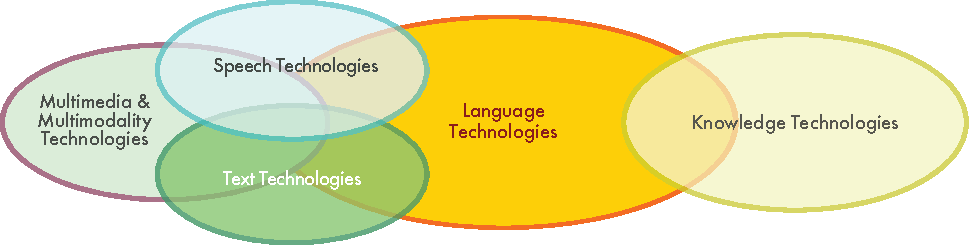
\includegraphics[width=\textwidth]{../_media/english/language_technologies}
  \caption{Language technologies}
  \label{fig:ltincontext_en}
  \colorrule{grey3}{\textwidth}{1.5pt}
\end{figure*}

Language technology is an established area of research with an extensive set of introductory literature. The interested reader is referred to the following references:  \cite{jurafsky-martin01, manning-schuetze1, lt-world1, lt-survey1}.

Before discussing the above application areas, we will briefly describe the architecture of a typical LT system.

\subsection{Application Architectures}

Typical software applications for language processing consist of several components that mirror different aspects of language and of the task they implement. Figure~\ref{fig:textprocessingarch_en} displays a highly simplified architecture that can be found in a text processing system. The first three modules deal with the structure and meaning of the text input:
\begin{itemize}
\item Pre-processing: cleaning up the data, removing formatting, detecting the input language, replacing “5è” by “cinquè” for Catalan, etc.
\item Grammatical analysis: finding the verb and its objects, modifiers and other sentence elements etc.; detecting the sentence structure.
\item Semantic analysis: disambiguation (Which meaning of apple is the right one in a given context?), resolving anaphora and referring expressions like she, the car, etc.; representing the meaning of the sentence in a machine-readable way.
\end{itemize}

\begin{figure*}[b]
  \colorrule{grey3}{\textwidth}{1.5pt}
  \center
  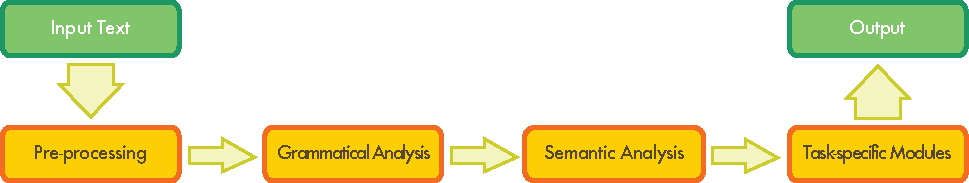
\includegraphics[width=\textwidth]{../_media/english/text_processing_app_architecture}
  \caption{A typical text processing architecture}
  \label{fig:textprocessingarch_en}
  \colorrule{grey3}{\textwidth}{1.5pt}
\end{figure*}

Task-specific modules then perform many different operations such as automatic summarisation of an input text, database lookups and many others. Below, we will illustrate core application areas and highlight their core modules. Again, the architectures of the applications are highly simplified and idealised, to illustrate the complexity of Language Technology (LT) applications in a generally understandable way. The most important tools and resources involved are set in bold text in the text and can also be found in the table at the end of the chapter.  The sections discussing the core application areas also contain an overview of the industries active in the respective field in Catalonia. 

After introducing the core application areas, we will give a short overview of the situation in LT research and education, concluding with an overview of past and ongoing research programs. At the end of this section, we will present an expert estimation on the situation regarding core LT tools and resources on a number of dimensions such as availability, maturity, or quality. This table gives a good overview on the situation of LT for Catalan.

\subsection{Core Application Areas}

    In this section, we focus on the most important LT tools and resources, and give an overview of LT activities in Catalan. Tools and resources that are set in bold in the text can also be found in the table at the end of this chapter.

\subsubsection{Language Checking}

Anyone using a word processing tool such as Microsoft Word has come across a spell checking component that indicates spelling mistakes and proposes corrections. Forty years after the first spelling correction program by Ralph Gorin, language checkers nowadays do not simply compare the list of extracted words against a dictionary of correctly spelled words, but have become increasingly sophisticated. 

\begin{figure*}[htb]
  \colorrule{grey3}{\textwidth}{1.5pt}
  \center
  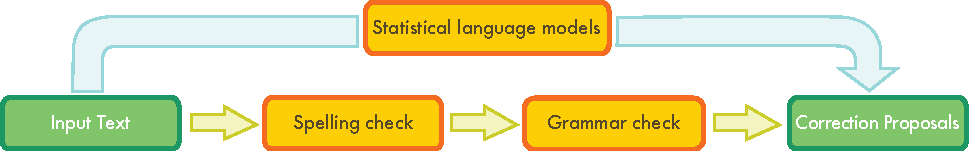
\includegraphics[width=\textwidth]{../_media/english/language_checking}
  \caption{Language checking (top: statistical; bottom: rule-based)}
  \label{fig:langcheckingaarch_en}
  \colorrule{grey3}{\textwidth}{1.5pt}
\end{figure*}

In addition to language-dependent algorithms for handling morphology (e.g. plural formation), some are now capable of recognising syntax–related errors, such as a missing verb or a verb that does not agree with its subject in person and number, e.g. in ‘She write a letter.’ 

Language checking (see figure~\ref{fig:langcheckingaarch_en}) either requires the formulation of language-specific grammar rules, i.e. a high degree of expertise and manual labour, or the use of a so-called statistical language model. Such models calculate the probability of a particular word occurring in a specific environment (i.e., the preceding and following words).

For example, ``llibre anglès'' is a much more probable word sequence than ``llibre anglesa''. A statistical language model can be automatically derived using a large amount of (correct) language data (i.e. a corpus). Up to now, these approaches have mostly been developed and evaluated on English language data. However, they do not necessarily transfer straightforwardly to Catalan with its flexible word order and richer inflection. 

The use of Language Checking is not limited to word processing tools. It is also applied in authoring support systems. Accompanying the rising number of technical products, the amount of technical documentation has rapidly increased over the last decades. Fearing customer complaints about wrong usage and damage claims resulting from bad or badly understood instructions, companies have begun to focus increasingly on the quality of technical documentation, and at the same time targeting the international market. Advances in natural language processing lead to the development of authoring support software, which assists the writer of technical documentation to use vocabulary and sentence structures consistent with certain rules and (corporate) terminology restrictions.

\boxtext{Language checking is not limited to word processors but also applies to authoring systems.}

Only a few companies and Language Service Providers offer products in this area for Catalan. Enciclopèdia Catalana, Maxigrammar and Inèdit have created and commercialised products that include spell and grammar checking for Catalan, as well as specific checking facilities adapted to different domains and styles. Softcatalà and Barcelona Media have also developed language tools that are offered to the community as web applications. A new version of “\textit{El Corrector}” has recently been developed and commercialised as iPod, iPhone and iPad apps. 

Besides spell checkers and authoring support, Language Checking is also important in the field of computer-assisted language learning and is applied to automatically correct queries sent to Web Search engines, e.g. Google’s ‘Did you mean…’ suggestions. 

\subsubsection{Web Search}

\begin{figure*}[htb]
  \colorrule{grey3}{\textwidth}{1.5pt}
  \center
  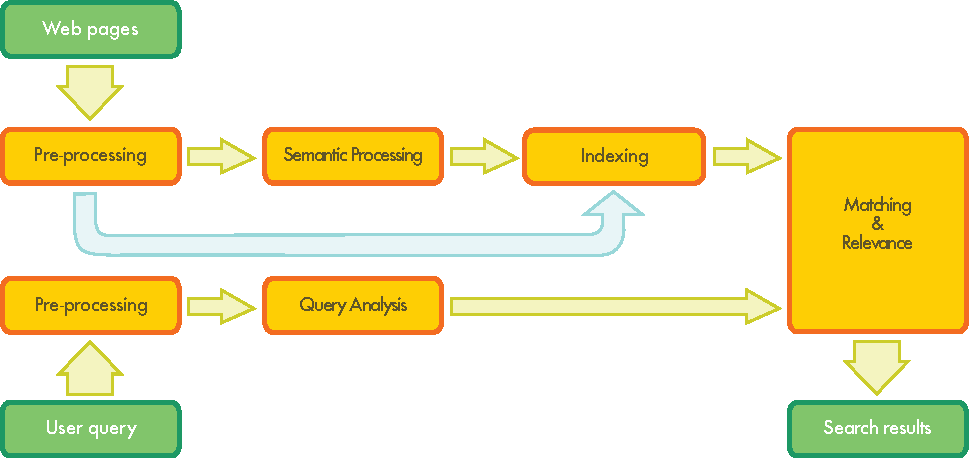
\includegraphics[width=\textwidth]{../_media/english/web_search_architecture}
  \caption{Web search architecture}
  \label{fig:websearcharch_en}
  \colorrule{grey3}{\textwidth}{1.5pt}
 \end{figure*}

Search on the web, in intranets or in digital libraries, is probably the most widely used and yet underdeveloped Language Technology today. The search engine Google, which started in 1998, is nowadays used for about 80\% of all search queries world-wide \cite{CAT-Nota22}. 

Neither the search interface nor the presentation of the retrieved results has significantly changed since the first version. In the current version, Google offers a spelling correction facility for misspelled words, including Catalan, and, in 2009, they incorporated basic semantic search capabilities into their algorithmic mix \cite{CAT-Nota23}, which can improve search accuracy by analysing the meaning of the query terms in context. The success story of Google shows that with a lot of data at hand and efficient techniques for indexing these data, a mainly statistically-based approach can lead to satisfactory results. 

However, for a more sophisticated request for information, integrating deeper linguistic knowledge is essential. In the research labs, experiments using machine-readable thesauri and ontological language resources like WordNet have shown improvements by allowing the possibility of finding a page on the basis of synonyms of the search terms, or even more loosely related terms. Again, these developments require language specific resources. A Catalan WordNet has been developed by the research centre TALP at Universitat Politècnica de Catalunya. The Catalan WordNet is freely available \cite{CAT-Nota24}.

\boxtext{The next generation of search engines\\ will have to include much more sophisticated language technology.}

The next generation of search engines will have to include much more sophisticated Language Technology. If a search query consists of a question or another type of sentence rather than a list of keywords, retrieving relevant answers to this query requires an analysis of this sentence on a syntactic and semantic level as well as the availability of an index that allows for a fast retrieval of the relevant documents. For example, imagine a user inputs the query ‘Give me a list of all companies that were taken over by other companies in the last five years’. For a satisfactory answer, \textbf{syntactic parsing} needs to be applied to analyse the grammatical structure of the sentence and determine that the user is looking for companies that have been taken over and not companies that took over others. Also, the expression last five years needs to be processed in order to find out which years it refers to. 

Finally, the processed query needs to be matched against a huge amount of unstructured data in order to find the piece or pieces of information the user is looking for. This is commonly referred to as information retrieval and involves the search for and ranking of relevant documents. In addition, generating a list of companies, we also need to extract the information that a particular string of words in a document refers to a company name. This kind of information is made available by so-called named-entity recognizers. 

Even more demanding is the attempt to match a query to documents written in a different language. For cross-lingual information retrieval, we have to automatically translate the query to all possible source languages and transfer the retrieved information back to the target language. The increasing percentage of data available in non-textual formats drives the demand for services enabling multimedia information retrieval, i.e., information search on images, audio, and video data. For audio and video files, this involves a \textbf{speech recognition} module to convert speech content into text or a phonetic representation, to which user queries can be matched.

Small and Medium Enterprises such as Inbenta \cite{CAT-inbenta} or RightNow (formerly q-go \cite{CAT-rightnow}) offer specific semantic search engines, including those that are developed for Catalan.

There are also some interesting initiatives to group specific web search services for Catalan, such as CerCat or Som-hi \cite{CAT-cercadors}, as one of the firs initiatives. An historical overview can be found at \cite{CAT-Resum-sobre-cercadors}.

\subsubsection{Speech Interaction}

\begin{figure*}[htb]
  \colorrule{grey3}{\textwidth}{1.5pt}
  \center
  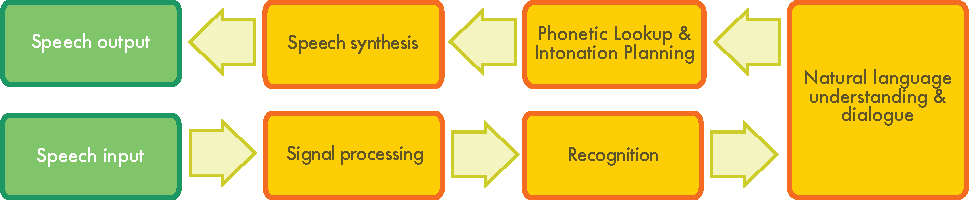
\includegraphics[width=\textwidth]{../_media/english/simple_speech-based_dialogue_architecture}
  \caption{Speech-based dialogue system}
  \label{fig:dialoguearch_en}
  \colorrule{grey3}{\textwidth}{1.5pt}
\end{figure*}

Speech interaction technology is the basis for the creation of interfaces that allow a user to interact with machines using spoken language rather than, e.g., a graphical display, a keyboard and a mouse. Today, such voice user interfaces (VUIs) are usually employed for partially or fully automating service offerings provided by companies to their customers, employees or partners via the telephone. Business domains that rely heavily on VUIs are banking, logistics, public transportation and telecommunications. Other usages of speech interaction technology are interfaces to particular devices, e.g. in-car navigation systems, and the employment of spoken language as an alternative to the input/output modalities of graphical user interfaces, e.g. in smart phones.

At its core, speech interaction comprises the following four different technologies:
\begin{itemize}
\item Automatic \textbf{speech recognition} (ASR) is responsible for determining which words were actually spoken given a sequence of sounds uttered by a user.
\item \textbf{Syntactic analysis} and \underline{semantic interpretation} deal with analysing the syntactic structure of a user’s utterance and interpret-ting the latter according to the given system’s purpose.
\item \textbf{Dialogue Management} is required for determining, on the part of the system the user interacts with, which action shall be taken given the user’s input and the system’s functionality.
\item \textbf{Speech Synthesis} (Text-to-Speech, TTS) technology is employed for transforming the wording of that utterance into sounds that will be output to the user. 
\end{itemize}
One of the major challenges is to have an ASR system recognise the words uttered by a user as precisely as possible. This requires either a restriction of the range of possible user utterances to a limi-ted set of keywords, or the manual creation of language models that cover a large range of natural language user utterances. Whereas the former results in a rather rigid and inflexible usage of a VUI and possibly causes a poor user acceptance, the creation, tuning and maintenance of language models may increase the costs significantly. However, VUIs that employ language models and initially allow a user to flexibly express their intent – evoked, e.g., by a \textit{How may I help you} greeting – show both a higher automation rate and a higher user acceptance and may therefore be considered as advantageous over a less flexible \textit{directed dialogue} approach.

\boxtext{Speech interaction is the basis for interfaces that allow a user to interact with spoken language.}

For the output part of a VUI, companies tend to use utterances pre-recorded by professional – ideally corporate – speakers a lot. For static utterances, in which the wording does not depend on the particular contexts of use or the personal data of the given user, this will result in a rich user experience. However, the more dynamic content an utterance needs to consider, the more the user experience may suffer from a poor prosody resulting from concatenating single audio files. In contrast, today’s TTS systems prove superior, though optimisable, regarding the prosodic naturalness of dynamic utterances.  

Regarding the market for speech interaction technology, the last decade has been characterised by a strong standardisation of the interfaces between the different technology components, as well as by standards for creating particular software artefacts for a given application. There also has been strong market consolidation within the last ten years, particularly in the field of ASR and TTS. Here, the national markets in the G20 countries – i.e. economically strong countries with a considerable population - are dominated by less than 5 players worldwide, with Nuance being the most prominent one in Europe, also for Catalan, although some smaller local companies are starting to compete, such as Verbio \cite{CAT-Nota25}, which is a spin-off of Universitat Politècnica de Catalunya and has its own speech technology. 

Regarding dialogue management technology and know-how, markets are strongly dominated by national players, which are usually SMEs. Most of the companies on the Catalan TTS market are essentially application developers. Key players in the Spanish market are: Indsys \cite{CAT-Nota26} (Intelligent Dialogue Systems), Fonetic \cite{CAT-Nota27}, Ydilo \cite{CAT-Nota28} and NaturalVoz \cite{CAT-Nota29}.

Looking beyond today’s state of technology, there will be significant changes due to the spread of smart phones as a new platform for managing customer relationships – in addition to the telephone, internet, and email channels. This tendency will also affect the employment of technology for speech interaction. On one hand, demand for telephony-based VUIs will decrease, in the long run. On the other hand, the usage of spoken language as a user-friendly input modality for smart phones will gain significant importance. This tendency is supported by the observable improvement of speaker independent speech recognition accuracy for speech dictation services that are already offered as centralised services to smart phone users. Given this ‘outsourcing’ of the recognition task to the infrastructure of applications, the application-specific employment of linguistic core technologies will supposedly gain importance compared to the present situation. 

\subsubsection{Machine Translation}

The idea of using digital computers for translation of natural languages came up in 1946 by A. D. Booth and was followed by substantial funding for research in this area in the 1950s and beginning again in the 1980s. Nevertheless, \textbf{Machine Translation} (MT) still fails to fulfil the high expectations it gave rise to in its early years. 

\boxtext{At its basic level, Machine Translation simply substitutes words in one natural language with words in another language.}

\begin{figure*}[htb]
  \colorrule{grey3}{\textwidth}{1.5pt}
  \center
  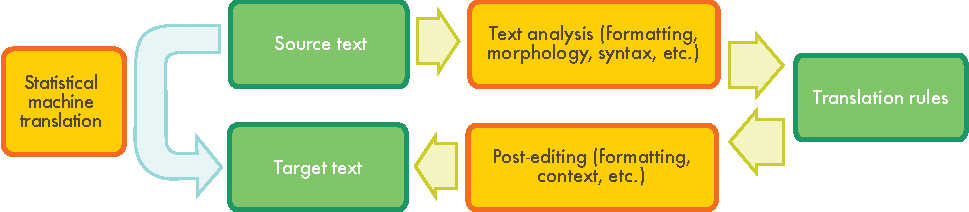
\includegraphics[width=\textwidth]{../_media/english/machine_translation}
  \caption{Machine translation (left: statistical; right: rule-based)}
  \label{fig:mtarch_en}
  \colorrule{grey3}{\textwidth}{1.5pt}
\end{figure*}

At its basic level, MT simply substitutes words in one natural language by words in another. This can be useful in subject domains with a very restricted, formulaic language, e.g., weather reports or for closely related languages. However, for a good translation of less standardised texts, larger text units (phrases, sentences, or even whole passages) need to be matched to their closest counterparts in the target language. The major difficulty here lies in the fact that human language is ambiguous, which yields challenges on multiple levels, e.g., word sense disambiguation at the lexical level (‘Jaguar’ can mean a car or an animal) or the attachment of prepositional phrases on the syntactic level as in:
\begin{itemize}
\item \textit{Passejava amb el nen cantant.}
\item \textit{T1: I was walking with the singer child.}
\item \textit{T2: I was walking and singing with the child.}
\end{itemize}

One way of approaching the task is based on linguistic rules. For translations between closely related languages, a direct translation may be feasible in cases like the example above. But often rule-based (or knowledge-driven) systems analyse the input text and create an intermediary, symbolic representation, from which the text in the target language is generated. The success of these methods is highly dependent on the availability of extensive \textbf{lexica} with morphological, syntactic, and semantic information, and large sets of \textbf{grammar rules} carefully designed by a skilled linguist.

Beginning in the late 1980s, as computational power increased and became less expensive, more interest was shown in statistical mo-dels for MT. The parameters of these statistical models are derived from the analysis of bilingual text corpora, such as the Europarl parallel corpus, which contains the proceedings of the European Parliament in 21 European languages. Given enough data, statistical MT works well enough to derive an approximate meaning of a foreign language text. However, unlike knowledge-driven systems, statistical (or data-driven) MT often generates ungrammatical output. On the other hand, besides the advantage that less human effort is required for grammar writing, data-driven MT can also cover particularities of the language that go missing in knowledge-driven systems, for example idiomatic expressions. 

As the strengths and weaknesses of knowledge- and data-driven MT are complementary, researchers nowadays unanimously target hybrid approaches combining methodologies of both. This can be done in several ways. One is to use both knowledge- and data-driven systems and have a selection module decide on the best output for each sentence. However, for longer sentences, no result will be perfect. A better solution is to combine the best parts of each sentence from multiple outputs, which can be fairly complex, as corresponding parts of multiple alternatives are not always obvious and need to be aligned. 

Due to the particular official situation of bilingualism in particular regions of Spain, and to the linguistic relatedness of Catalan with Spanish, the development of MT systems for this pair of languages has been quite successful. Initially supported by the autonomous Catalan leading MT systems like METAL (Siemens), ATLAS (Fujitsu) were located in Barcelona during the 1990’s, and when the big companies ended their engagement, the systems were further developed by offspring and spin-off companies: METAL was further developed by a local SME, INCYTA, as well as by GMS and later by Lucy Software, which is currently the main (but not the only) vendor for MT systems involving Catalan. In fact, the Catalan-Spanish MT system  bought by the Generalitat of Catalonia was offered as a public web service as early as 2005, while Google started offering it in 2007. 

Other companies also developed MT systems with in-house technologies: T6 Estàndar Linguistic and AutomaticTrans. The system developed by AutomaticTrans has its origin in the production of a bilingual newspaper, in Catalan and Spanish, El Periódico. Currently, there are three newspapers which are made available in the two languages  through the use of Machine Translation technology. The other two are El Segre and La Vanguardia. 

The Generalitat Valenciana supported the creation of a MT system specific for Valencian, SALT. More recently, the Universidad Politécnica de Valencia has also released a version of SiShiTra, a hybrid system, and the open-source OpenTrad also offers a particular version for Valencian.

The pair Spanish-Catalan was the origin of the open source system developed by the Transducens \cite{CAT-transducens} group of the Universitat d'Alacant \cite{CAT-UnivAlacant}, Apertium, which is the first open-source MT technology in the world. Its commercial exploitation is mainly carried out by Prompsit Language Engineering and OpenTrad Consortium. 

Most of the systems introduced above are rule-based. While there is significant research on this technology in national and international contexts, data-driven and hybrid systems have been less successful in business than in research so far. 

Provided with good adaptation in terms of user-specific terminology and workflow integration, the use of MT can increase productivity significantly. Thus, the main user of MT for Catalan is the public administration, including the Justice Department and other Ministries, since the beginning of the 21st century. 

The quality of MT systems is still considered to have huge improvement potential. Challenges include the adaptability of the language resources to a given subject domain or user area and the integration into existing workflows with term bases and translation memories.

In addition, most of the existing parallel corpora are between Spanish and Catalan, so for the majority of translation solutions, Spanish is the pivot language.

Evaluation campaigns help to compare the quality of MT systems, their approaches and the status of the systems for different language pairs. Figure~\ref{fig:euromatrix_en} (p.~\pageref{fig:euromatrix_en}), which was prepared during the Euromatrix+ project, shows the pair-wise performances obtained for 22 of the 23 EU languages (Irish was not compared). The results are ranked according to a BLEU score, which indicates higher scores for better translations \cite{bleu1}. A human translator would normally achieve around 80 points. The best results (in green and blue) were achieved by languages that benefit from a considerable research effort in coordinated programmes and the existence of many parallel corpora (e.\,g., English, French, Dutch, Spanish and German). The languages with poorer results are shown in red. These either lack such development efforts or are structurally very different from other languages (e.\,g., Hungarian, Maltese, Finnish).

\subsection{Other Application Areas}

Building Language Technology applications involves a range of subtasks that do not always surface at the level of interaction with the user, but provide significant service functionalities ‘under the hood’ of the system. Therefore, they constitute important research issues that have become individual sub-disciplines of Computational Linguistics in academia. 

Question answering has become an active area of research, for which annotated corpora have been built and scientific competitions have been started.

The idea is to move from keyword-based search (to which the engine responds with a whole collection of potentially relevant documents) to the scenario of the user asking a concrete question and the system providing a single answer: \\
\begin{itemize}
\item[] \textit{Question: At what age did Neil Armstrong step on the moon?}
\item[] \textit{Answer: 38.}
\end{itemize}

While this is obviously related to the aforementioned core area Web Search, question answering nowadays is primarily an umbrella term for research questions such as what types of questions should be distinguished and how should they be handled, how can a set of documents that potentially contain the answer be analysed and compared (do they give conflicting answers?), and how can specific information - the answer - be reliably extracted from a document, without unduly ignoring the context. 

\boxtext{Language technology applications often provide significant service functionalities behind the scenes of larger software systems.}

This is in turn related to the information extraction (IE) task, an area that was extremely popular and influential at the time of the ‘statistical turn’ in Computational Linguistics, in the early 1990s. IE aims at identifying specific pieces of information in specific classes of documents; this could e.g. be the detection of the key players in company takeovers as reported in newspaper stories. Another scenario that has been worked on is reports on terrorist incidents, where the problem is to map the text to a template specifying the perpetrator, the target, time and location of the incident, and the results of the incident. Domain-specific template-filling is the central characteristic of IE, which for this reason is another example of a ‘behind the scenes’ technology that constitutes a well-demarcated research area but for practical purposes then needs to be embedded into a suitable application environment. 

Two ‘borderline’ areas, which sometimes play the role of standalone application and sometimes that of supportive, ‘under the hood’ component are text summarization and text generation. Summarization, obviously, refers to the task of making a long text short, and is offered for instance as a functionality within MS Word. It works largely on a statistical basis, by first identifying ‘important’ words in a text (that is, for example, words that are highly frequent in this text but markedly less frequent in general language use) and then determining those sentences that contain many important words. These sentences are then marked in the document, or extracted from it, and are taken to constitute the summary. In this scenario, which is by far the most popular one, summarization equals sentence extraction: the text is reduced to a subset of its sentences. All commercial summarizers make use of this idea. An alternative approach, to which some research is devoted, is to actually synthesize new sentences, i.e., to build a summary of sentences that need not show up in that form in the source text. This requires a certain amount of deeper understanding of the text and therefore is much less robust. All in all, a text generator is in most cases not a stand-alone application but embedded into a larger software environment, such as into the clinical information system where patient data is collected, stored and processed, and report generation is just one of many functionalities.

\boxtext{For Catalan and for most languages, research in most text technologies is much less developed than for English.}

The situation in all these research areas for most of the languages is much less developed than it is for English, where question answering, information extraction, and summarization have since the 1990s been the subject of numerous open competitions, primarily those organised by DARPA/NIST in the United States. These have significantly improved the state of the art, but the focus has always been on English; some competitions have added multilingual tracks, but Catalan has never been prominent. Accordingly, there are hardly any annotated corpora or other resources for Catalan that relate to these tasks. Summarization systems, when using purely statistical methods, are often to a good extent language-independent, and thus some research prototypes are available. For text generation, reusable components have traditionally been limited to the surface realisation modules (the "generation grammars"); again, most available software is for English.

\subsection{Educational Programmes}

Language Technology is a highly interdisciplinary field, involving the expertise of linguists, computer scientists, mathematicians, philosophers, psycholinguists, and neuroscientists, among others. Although it has not yet acquired a fixed place in any of the faculty systems of the universities in the Catalan linguistic domain, Barcelona has a higher concentration of studies that consider the field. 
Several subjects related to language technology are offered in bachelor degrees by different departments, such as the faculty of computer science (e.g., in the Universitat d’Alacant) or the faculty of linguistics (e.g., in the Universitat de Barcelona, the Universitat PompeuFabra and the Universitat Oberta de Catalunya).
As regards masters courses and postgraduate degrees, Universitat Autònoma de Barcelona offers the International Master in Natural Language Processing and Human Language Technology, in collaboration with foreign universities. Besides this, some masters are offered in which one of the research areas focusses on natural language processing (e.g., the Universitat de Barcelona, the Universitat Pompeu Fabra, the Universitat de Girona and the Universitat Rovira i Virgili). Modules in Language Technology are also offered to students of other master courses (e.g. the Universitat d’Alacant, the Universitat de Castelló and the Universitat Politècnica de València). 
PhD programmes are also offered, in which one of the research areas is human language technologies (e.g. the Universitat d’Alacant, the Universitat de Barcelona and the Universitat Rovira i Virgili).

\subsection{National Projects and Efforts}

Technology programs for the Catalan language have been supported by the Spanish and the Catalan Governments.

The existence of comparably lively LT activity, specifically in the Barcelona area, can be traced back to major LT programs and large research projects carried out in the last decades. One of the first programs was EUROTRA, the ambitious Machine Translation (MT) project established and funded by the European Commission from the late 1970s until 1994. Even though the EUROTRA project did not work with Catalan, the project, which had a long-term impact on language industries in Europe, was also crucial to highlighting the importance of languages in the technological world, and how it could affect small to medium languages. The Catalan government quickly began to understand the challenges and initiated different programs that basically addressed the localization of differrent software tools, including LT applications. 

Machine translation, speech recognition, spelling and grammar checking research and industrial developments have been supported by different departments of the Generalitat de Catalunya for more than 20 years. The Secretaria de Política Lingüística, the Comissionat per a la Societat de la Informació and the Secretaria de Telecomunicacions i Societat de la Informació have been the main engines of the support policies. Besides, MT into or from Catalan has also benefited from Spanish funding programs. Projects such as Apertium (open source MT system) and OpenTrad, as well as a number of other small programs, have received funding from the Ministerio de Ciencia y Tecnología. 

The CREL – Centre de Referència en Enginyeria Lingüística, 1996-2000, managed by the Institut d’Estudis Catalans and with participants from the major Catalan Universities, was created with the specific aim of promoting the creation of resources and tools for the automatic processing of Catalan texts in a variety of applications. 

As regards the presence of the Catalan language in European infrastructures, in 2008 the Catalan Government signed an agreement with Universitat Pompeu Fabra, the national representative of the European project CLARIN in Spain, with the aim of building a Catalan demonstrator. The main goal of this demonstrator (CLARIN-CAT-LAB), which is already available for research purposes \cite{CAT-Nota30}, is to integrate language resources and technology for the Catalan language, thus guaranteeing the presence of this language in the European CLARIN infrastructure. In addition, the Biblioteca de Catalunya, Catalonia’s national library, is one of the partners in the EUROPEANA project. Other Catalan institutions are also contributing content to the project.

From 2000 up until the present day, the Spanish Government supported several projects in the area of multilingual speech technologies within the National Plan of Research and Technology, i.e., TEHAM, AVIVAVOZ, and BUCEADOR. The main purpose of these projects was to improve the quality of speech recognition, speech translation and text to speech synthesis in all the official languages spoken in Spain, i.e., Basque, Galician, Catalan and Spanish.

In 2005, the Catalan Government launched a project to produce Language Resources for Speech Recognition and Speech Synthesis. As a result, Language Resources for telephone applications, in-car applications and microphone applications were produced. Later, the project TECNOPARLA (2007-2010) had as its objective the translation of speech between Spanish and Catalan. The speech signals were collected directly from TV programmes. The project resulted on advances in all the component speech technologies, i.e.  diarization, speech recognition, speech translation and text to speech synthesis.
  
\subsection{Availability of Tools and Resources}

    The following table summarises the current state of language technology support for the German language. The rating for existing tools and resources was generated by leading experts in the field who provided estimates based on a scale from 0 (very low) to 6 (very high) according to seven criteria.

\begin{figure*}[htb]
\centering
%\begin{tabular}{>{\columncolor{orange1}}p{.33\linewidth}ccccccc} % ORIGINAL
\begin{tabular}{>{\columncolor{orange1}}p{.33\linewidth}@{\hspace*{6mm}}c@{\hspace*{6mm}}c@{\hspace*{6mm}}c@{\hspace*{6mm}}c@{\hspace*{6mm}}c@{\hspace*{6mm}}c@{\hspace*{6mm}}c}
\rowcolor{orange1}
 \cellcolor{white}&\begin{sideways}\makecell[l]{Quantity}\end{sideways}
&\begin{sideways}\makecell[l]{\makecell[l]{Availability} }\end{sideways} &\begin{sideways}\makecell[l]{Quality}\end{sideways}
&\begin{sideways}\makecell[l]{Coverage}\end{sideways} &\begin{sideways}\makecell[l]{Maturity}\end{sideways} &\begin{sideways}\makecell[l]{Sustainability}\end{sideways} &\begin{sideways}\makecell[l]{Adaptability}\end{sideways} \\ \addlinespace
\multicolumn{8}{>{\columncolor{orange2}}l}{Language Technology: Tools, Technologies and Applications} \\ \addlinespace
Speech Recognition	&3&3&3&3&3&3&2 \\ \addlinespace
Speech Synthesis &4&2&4&4&5&4&2\\ \addlinespace
Grammatical analysis &3&2.5&4&4&4&2.5&2.5\\ \addlinespace
Semantic analysis &1&1&2&1&1&1&1\\ \addlinespace
Text generation &1&2&3&1&3&3&1\\ \addlinespace
Machine translation &3&3&2&3&4&1&2\\ \addlinespace
\multicolumn{8}{>{\columncolor{orange2}}l}{Language Resources: Resources, Data and Knowledge Bases} \\ \addlinespace
Text corpora &3&2.5&3.5&3&3&2.5&2.5\\ \addlinespace
Speech corpora &3&5&3&2&3&3&2\\ \addlinespace
Parallel corpora &2&1&2&2&2&1&1\\ \addlinespace
Lexical resources &2.5&2&3&2.5&3&3&2.5\\ \addlinespace
Grammars &2&3&2&2&2&2&2\\
\end{tabular}
\caption{State of language technology support for Catalan}
\label{fig:lrlttable_en}
\end{figure*}

The table can be summarized in the form of a number of key messages, which highlight crucial issues for the further development of automatic language processing of Catalan, on the basis of the present situation:

\begin{itemize}
\item While some specific corpora of high quality exist, a very large syntactically annotated corpus is not available.
\item For Catalan, a large corpus exists, but it is not easily/cheaply accessible.
\item Many of the resources lack standardisation, i.e., even if they exist, sustainability is not given; concerted programs and initiatives are needed to standardise data and interchange formats.
\item Semantics is more difficult to process than syntax; text semantics is more difficult to process than word and sentence semantics.
\item The more semantics a tool takes into account, the more difficult it is to find the right data; more efforts for supporting deep processing are needed.
\item Standards do exist for semantics in the sense of world knowledge (RDF, OWL, etc.); they are, however, not easily applicable to NLP tasks.
\item Speech processing is currently more mature than NLP for written text.
\item There are many groups working in machine translation, particularly focused in Catalan-Spanish. 
\item Research has been successful in designing particular high quality software, but it is nearly impossible to come up with sustainable and standardised solutions, given the current funding situations.
\end{itemize}

\subsection{Cross-language comparison}

    The current state of LT support varies considerably from one language community to another. In order to compare the situation between languages, this section will present an evaluation based on two sample application areas (machine translation and speech processing) and one underlying technology (text analysis), as well as basic language resources needed for building LT applications. 

\begin{figure*}[tb]
  \small
  \centering
  \begin{tabular}
  { % defines color for each column.
  >{\columncolor{corange5}}p{.13\linewidth}@{\hspace{.040\linewidth}}
  >{\columncolor{corange4}}p{.13\linewidth}@{\hspace{.040\linewidth}}
  >{\columncolor{corange3}}p{.13\linewidth}@{\hspace{.040\linewidth}}
  >{\columncolor{corange2}}p{.13\linewidth}@{\hspace{.040\linewidth}}
  >{\columncolor{corange1}}p{.13\linewidth} 
  }
\rowcolor{orange1} % redefines color for all columns in row 1
\begin{center}\vspace*{-2mm}\textbf{Excellent}\end{center} & 
\begin{center}\vspace*{-2mm}\textbf{Good}\end{center} & 
\begin{center}\vspace*{-2mm}\textbf{Moderate}\end{center} & 
\begin{center}\vspace*{-2mm}\textbf{Fragmentary}\end{center} & 
\begin{center}\vspace*{-2mm}\textbf{Weak/no}\end{center} \\ \addlinespace
  
& \vspace*{0.5mm}English
& \vspace*{0.5mm}
Czech \newline 
Dutch \newline 
Finnish \newline 
French \newline 
German \newline   
Italian \newline  
Portuguese \newline 
Spanish \newline
& \vspace*{0.5mm}Basque \newline 
Bulgarian \newline 
\textbf{Catalan} \newline 
Danish \newline 
Estonian \newline 
Galician\newline 
Greek \newline  
Hungarian  \newline
Irish \newline  
Norwegian \newline 
Polish \newline 
Serbian \newline 
Slovak \newline 
Slovene \newline 
Swedish \newline
& \vspace*{0.5mm}
Croatian \newline 
Icelandic \newline  
Latvian \newline 
Lithuanian \newline 
Maltese \newline 
Romanian\\
\end{tabular}
\caption{Speech processing: state of language technology support for 30 European languages}
\label{fig:speech_cluster_en}
\end{figure*}

\begin{figure*}[tb]
  \small
  \centering
  \begin{tabular}
  { % defines color for each column.
  >{\columncolor{corange5}}p{.13\linewidth}@{\hspace{.040\linewidth}}
  >{\columncolor{corange4}}p{.13\linewidth}@{\hspace{.040\linewidth}}
  >{\columncolor{corange3}}p{.13\linewidth}@{\hspace{.040\linewidth}}
  >{\columncolor{corange2}}p{.13\linewidth}@{\hspace{.040\linewidth}}
  >{\columncolor{corange1}}p{.13\linewidth} 
  }
\rowcolor{orange1} % redefines color for all columns in row 1
\begin{center}\vspace*{-2mm}\textbf{Excellent}\end{center} & 
\begin{center}\vspace*{-2mm}\textbf{Good}\end{center} & 
\begin{center}\vspace*{-2mm}\textbf{Moderate}\end{center} & 
\begin{center}\vspace*{-2mm}\textbf{Fragmentary}\end{center} & 
\begin{center}\vspace*{-2mm}\textbf{Weak/no}\end{center} \\ \addlinespace
  
& \vspace*{0.5mm} English 
& \vspace*{0.5mm} 
French \newline 
Spanish
& \vspace*{0.5mm}
\textbf{Catalan} \newline 
Dutch \newline 
German \newline 
Hungarian \newline
Italian \newline 
Polish \newline 
Romanian \newline 
& \vspace*{0.5mm}Basque \newline 
Bulgarian \newline 
Croatian \newline 
Czech \newline
Danish \newline 
Estonian \newline 
Finnish \newline 
Galician \newline 
Greek \newline 
Icelandic \newline 
Irish \newline 
Latvian \newline 
Lithuanian \newline 
Maltese \newline 
Norwegian \newline 
Portuguese \newline 
Serbian \newline 
Slovak \newline 
Slovene \newline 
Swedish \newline 
\end{tabular}
\caption{Machine translation: state of language technology support for 30 European languages}
\label{fig:mt_cluster_en}
\end{figure*}

\begin{figure*}[tb]
  \small
  \centering
  \begin{tabular}
  { % defines color for each column.
  >{\columncolor{corange5}}p{.13\linewidth}@{\hspace{.040\linewidth}}
  >{\columncolor{corange4}}p{.13\linewidth}@{\hspace{.040\linewidth}}
  >{\columncolor{corange3}}p{.13\linewidth}@{\hspace{.040\linewidth}}
  >{\columncolor{corange2}}p{.13\linewidth}@{\hspace{.040\linewidth}}
  >{\columncolor{corange1}}p{.13\linewidth} 
  }
\rowcolor{orange1} % redefines color for all columns in row 1
\begin{center}\vspace*{-2mm}\textbf{Excellent}\end{center} & 
\begin{center}\vspace*{-2mm}\textbf{Good}\end{center} & 
\begin{center}\vspace*{-2mm}\textbf{Moderate}\end{center} & 
\begin{center}\vspace*{-2mm}\textbf{Fragmentary}\end{center} & 
\begin{center}\vspace*{-2mm}\textbf{Weak/no}\end{center} \\ \addlinespace

& \vspace*{0.5mm}English
& \vspace*{0.5mm}
  Dutch \newline 
  French \newline 
  German \newline 
  Italian \newline 
  Spanish
& \vspace*{0.5mm}Basque \newline 
  Bulgarian \newline 
  \textbf{Catalan} \newline 
  Czech \newline 
  Danish \newline 
  Finnish \newline 
  Galician \newline 
  Greek \newline 
  Hungarian \newline 
  Norwegian \newline 
  Polish \newline 
  Portuguese \newline 
  Romanian \newline 
  Slovak \newline 
  Slovene \newline 
  Swedish \newline 
& \vspace*{0.5mm}
  Croatian \newline 
  Estonian \newline 
  Icelandic \newline 
  Irish \newline 
  Latvian \newline 
  Lithuanian \newline 
  Maltese \newline 
  Serbian \\
  \end{tabular}
\caption{Text analysis: state of language technology support for 30 European languages}
\label{fig:text_cluster_en}
\end{figure*}

\begin{figure*}[tb]
  \small
  \centering
  \begin{tabular}
  { % defines color for each column.
  >{\columncolor{corange5}}p{.13\linewidth}@{\hspace{.040\linewidth}}
  >{\columncolor{corange4}}p{.13\linewidth}@{\hspace{.040\linewidth}}
  >{\columncolor{corange3}}p{.13\linewidth}@{\hspace{.040\linewidth}}
  >{\columncolor{corange2}}p{.13\linewidth}@{\hspace{.040\linewidth}}
  >{\columncolor{corange1}}p{.13\linewidth} 
  }
\rowcolor{orange1} % redefines color for all columns in row 1
\begin{center}\vspace*{-2mm}\textbf{Excellent}\end{center} & 
\begin{center}\vspace*{-2mm}\textbf{Good}\end{center} & 
\begin{center}\vspace*{-2mm}\textbf{Moderate}\end{center} & 
\begin{center}\vspace*{-2mm}\textbf{Fragmentary}\end{center} & 
\begin{center}\vspace*{-2mm}\textbf{Weak/no}\end{center} \\ \addlinespace
    
& \vspace*{0.5mm}English
& \vspace*{0.5mm} 
    Czech \newline 
    Dutch \newline 
    French \newline 
    German \newline 
    Hungarian \newline
    Italian \newline
    Polish \newline
    Spanish \newline
    Swedish \newline 
& \vspace*{0.5mm} Basque\newline 
    Bulgarian\newline 
    \textbf{Catalan} \newline 
    Croatian \newline 
    Danish \newline 
    Estonian \newline 
    Finnish \newline 
    Galician \newline 
    Greek \newline 
    Norwegian \newline 
    Portuguese \newline 
    Romanian \newline 
    Serbian \newline 
    Slovak \newline 
    Slovene \newline
&  \vspace*{0.5mm}
    Icelandic \newline 
    Irish \newline 
    Latvian \newline 
    Lithuanian \newline 
    Maltese  \\
  \end{tabular}
  \caption{Speech and text resources: State of support for 30 European languages}  
  \label{fig:resources_cluster_en}
\end{figure*}

The current state of LT support varies considerably from one language community to another. In order to compare the situation between languages, this section will present an evaluation based on two sample application areas (machine translation and speech processing) and one underlying technology (text analysis), as well as basic resources needed for building LT applications. The languages were categorised using the following five-point scale: 

\begin{enumerate}
\item Excellent support
\item Good support
\item Moderate support
\item Fragmentary support
\item Weak or no support
\end{enumerate}

LT support was measured according to the following criteria:

\textbf{Speech Processing:} Quality of existing speech recognition technologies, quality of existing speech synthesis technologies, coverage of domains, number and size of existing speech corpora, amount and variety of available speech-based applications.

\textbf{Machine Translation:} Quality of existing MT technologies, number of language pairs covered, coverage of linguistic phenomena and domains, quality and size of existing parallel corpora, amount and variety of available MT applications.

\textbf{Text Analysis:} Quality and coverage of existing text analysis technologies (morphology, syntax, semantics), coverage of linguistic phenomena and domains, amount and variety of available applications, quality and size of existing (annotated) text corpora, quality and coverage of existing lexical resources (e.\,g., WordNet) and grammars.

\textbf{Resources:} Quality and size of existing text corpora, speech corpora and parallel corpora, quality and coverage of existing lexical resources and grammars.

The above tables show that, thanks to LT funding programs from the Spanish and Catalonian governments in recent decades, the Catalan language is equipped as most of other European languages. It compares well with languages with a similar number of speakers such as Hungarian, Greek, and European Portuguese despite these are official languages of EU countries. But LT resources and tools for Catalan clearly do not yet reach the quality and coverage of comparable resources and tools for the Spanish language, which is in a good position in almost all LT areas. And there are still plenty of gaps in Spanish language resources with regard to high quality applications.

For speech processing, current technologies perform well enough to be successfully integrated into a number of industrial applications such as Interactive Voice Response systems and constrained domain dictation systems. Machine Translation systems get a good performance, especially between the language pairs Spanish-Catalan and English-Catalan. However, for building more sophisticated applications, such as machine translation, there is a clear need for resources and technologies that cover a wider range of linguistic aspects and allow a deep semantic analysis of the input text. By improving the quality and coverage of these basic resources and technologies, we shall be able to open up new opportunities for tackling a vast range of advanced application areas, including high-quality machine translation.  

\subsection{Conclusions}

    \emph{In this series of white papers, we have made an important initial effort to assess language technology support for 30 European languages, and provide a high-level comparison across these languages. By identifying the gaps, needs and deficits, the European language technology community and related stakeholders are now in a position to design a large scale research and development programme aimed at building a truly multilingual, technology-enabled Europe.}

The results of this white paper series show that there is a dramatic difference in language technology support between the various European languages. While there are good quality software and resources available for some languages and application areas, others (usually ‘smaller’ languages) have substantial gaps. Many languages lack basic technologies for text analysis and the essential resources for developing these technologies. Others have basic tools and resources but are as yet unable to invest in semantic processing. We therefore still need to make a large-scale effort to attain the ambitious goal of providing high-quality machine translation between all European languages. 

    In the case of the Catalan language, we are moderately optimistic about the current state of language technology support. There is a viable LT research community in Catalonia, which has been supported by Spanish and Catalan research programmes. A number of resources and state-of-the-art technologies have been produced and distributed for Catalan. However, the scope of the resources and the range of tools are still very limited when compared to the resources and tools for the Spanish language (and obviously for the English language) and they are simply not sufficient in quality and quantity to develop the kind of technologies required to support a truly multilingual knowledge society.

    The Catalan language technology industry dedicated to transforming research into products is currently very small. Most large companies have either stopped or severely cut their LT efforts, leaving the languages spoken by a small number of people in a secondary objective.

    Our findings show that the only alternative is to make a substantial effort to create LT resources for Catalan, and use them to drive forward research, innovation and development. The need for large amounts of data and the extreme complexity of language technology systems makes it vital to develop a new infrastructure and a more coherent research organization to spur greater sharing and cooperation.

    There is also a lack of continuity in research and development funding. Short-term coordinated programmes tend to alternate with periods of sparse or zero funding. In addition, there is an overall lack of coordination with programmes in other EU countries and at the European Commission level.

    We can therefore conclude that there is a desperate need for a large, coordinated initiative focused on overcoming the differences in language technology readiness for European languages as a whole.

    META-NET’s long-term goal is to introduce high-quality language technology for all languages in order to achieve political and economic unity through cultural diversity. The technology will help tear down existing barriers and build bridges between Europe’s languages. This requires all stakeholders - in politics, research, business, and society - to unite their efforts for the future. 
\end{multicols}

\clearpage


% --------------------------------------------------------------------------
\ssection[About META-NET]{About META-NET}

\begin{multicols}{2}
META-NET is a Network of Excellence funded by the European Commission. The network currently consists of 54 members from 33 European countries \cite{rehm2011}. META-NET fosters the Multilingual Europe Technology Alliance (META), a growing community of language technology professionals and organisations in Europe. META-NET cooperates with other initiatives like the Common Language Resources and Technology Infrastructure (CLARIN), which is helping to establish digital humanities research in Europe. META-NET fosters the technological foundations for a truly multilingual European information society that:

\begin{itemize}
\item makes communication and cooperation possible across languages;
\item provides equal access to information and knowledge in any language;
\item offers advanced and affordable networked information technology to European citizens.
\end{itemize}

META-NET stimulates and promotes multilingual technologies for all European languages. The technologies enable automatic translation, content production, information processing and knowledge management for a wide variety of applications and subject domains. The network wants to improve current approaches, so better communication and cooperation across languages can take place. Europeans have an equal right to information and knowledge regardless of language.

META-NET launched on 1 February 2010 with the goal of advancing research in language technology (LT). The network supports a Europe that unites as a single digital market and information space. META-NET has conducted several activities that further its goals. META-VISION, META-SHARE and META-RESEARCH are the network’s three lines of action.

\textbf{META-VISION} fosters a dynamic and influential stakeholder community that unites around a shared vision and a common strategic research agenda (SRA). The main focus of this activity is to build a coherent and cohesive LT community in Europe by bringing together representatives from highly fragmented and diverse groups of stakeholders. In the first year of META-NET, presentations at the FLaReNet Forum (Spain), Language Technology Days (Luxembourg), JIAMCATT 2010 (Luxembourg), LREC 2010 (Malta), EAMT 2010 (France) and ICT 2010 (Belgium) centred on public outreach. According to initial estimates, META-NET has already contacted more than 2,500 LT professionals to develop its goals and visions with them. At the META-FORUM 2010 event in Brussels, META-NET communicated the initial results of its vision building process to more than 250 participants. In a series of interactive sessions, the participants provided feedback on the visions presented by the network. 

\textbf{META-SHARE} creates an open, distributed facility for exchanging and sharing resources. The peer-to-peer network of repositories will contain language data, tools and web services that are documented with high-quality metadata and organised in standardised categories. The resources can be readily accessed and uniformly searched. The available resources include free, open source materials as well as restricted, commercially available, fee-based items. META-SHARE targets existing language data, tools and systems as well as new and emerging products that are required for building and evaluating new technologies, products and services. The reuse, combination, repurposing and re-engineering of language data and tools plays a crucial role. META-SHARE will eventually become a critical part of the LT marketplace for developers, localisation experts, researchers, translators and language professionals from small, mid-sized and large enterprises. META-SHARE addresses the full development cycle of LT—from research to innovative products and services. A key aspect of this activity is establishing META-SHARE as an important and valuable part of a European and global infrastructure for the LT community. 

\textbf{META-RESEARCH} builds bridges to related technology fields. This activity seeks to leverage advances in other fields and to capitalise on innovative research that can benefit language technology. In particular, this activity wants to bring more semantics into machine translation (MT), optimise the division of labour in hybrid MT, exploit context when computing automatic translations and prepare an empirical base for MT. META-RESEARCH is working with other fields and disciplines, such as machine learning and the Semantic Web community. META-RESEARCH focuses on collecting data, preparing data sets and organising language resources for evaluation purposes; compiling inventories of tools and methods; and organising workshops and training events for members of the community. This activity has already clearly identified aspects of MT where semantics can impact current best practices. In addition, the activity has created recommendations on how to approach the problem of integrating semantic information into MT. META-RESEARCH is also finalising a new language resource for MT, the Annotated Hybrid Sample MT Corpus, which provides data for English-German, English-Spanish and English-Czech language pairs. META-RESEARCH has also developed software that collects multilingual corpora that are hidden on the Web.
\end{multicols}

\vfill
\centerline{office@meta-net.eu -- http://www.meta-net.eu}

\cleardoublepage

\appendix
\addtocontents{toc}{\protect\bigskip}

\bsection[Referències -- References]{Referències --- References}
\bibliographystyle{unsrt} % What is the difference between "unsrt" und "is-unsrt"?
%\bibliographystyle{is-unsrt}
\bibliography{galician_references}
  
\cleardoublepage

\bsection[Membres de META-NET -- META-NET Members]{Membres de META-NET --- META-NET Members}
\label{metanetmembers}

\small

\begin{longtable}{@{}llp{113mm}@{}}
  Alemanya & \textcolor{grey1}{Germany} & Language Technology Lab, DFKI: Hans Uszkoreit, Georg Rehm\\ \addlinespace
  & & Human Language Technology and Pattern Recognition, RWTH Aachen University: Hermann Ney \\ \addlinespace
  & & Department of Computational Linguistics, Saarland University: Manfred Pinkal\\ \addlinespace Dänemark &  \textcolor{grey1}{Denmark} & Centre for Language Technology, University of Copenhagen: \newline Bolette Sandford Pedersen, Bente Maegaard\\ \addlinespace
  Àustria & \textcolor{grey1}{Austria} & Zentrum für Translationswissenschaft, Universität Wien: Gerhard Budin\\ \addlinespace 
  Bèlgica & \textcolor{grey1}{Belgium} & Computational Linguistics and Psycholinguistics Research Centre, University of Antwerp: Walter Daelemans\\ \addlinespace
  & & Centre for Processing Speech and Images, University of Leuven: Dirk van Compernolle \\ \addlinespace
  Bulgària & \textcolor{grey1}{Bulgaria} & Institute for Bulgarian Language, Bulgarian Academy of Sciences: Svetla Koeva \\ \addlinespace
  Croàcia & \textcolor{grey1}{Croatia} & Institute of Linguistics, Faculty of Humanities and Social Science, University of Zagreb: Marko Tadić \\ \addlinespace
  Eslovàquia & \textcolor{grey1}{Slovakia} & Ľudovít Štúr Institute of Linguistics, Slovak Academy of Sciences: Radovan Garabík \\ \addlinespace 
  Eslovènia & \textcolor{grey1}{Slovenia} & Jozef Stefan Institute: Marko Grobelnik \\ \addlinespace 
  Espanya & \textcolor{grey1}{Spain} & Barcelona Media: Toni Badia, Maite Melero \\ \addlinespace 
  & & Institut Universitari de Lingüística Aplicada, Universitat Pompeu Fabra: Núria Bel \\ \addlinespace 
  & & Aholab Signal Processing Laboratory, University of the Basque Country:\newline Inma Hernaez Rioja \\ \addlinespace 
  & & Center for Language and Speech Technologies and Applications, Universitat Politècnica de Catalunya:  Asunción Moreno \\ \addlinespace 
  & & Department of Signal Processing and Communications, University of Vigo:\newline Carmen García Mateo \\ \addlinespace 
  Estònia & \textcolor{grey1}{Estonia} & Institute of Computer Science, University of Tartu: Tiit Roosmaa, Kadri Vider\\ \addlinespace
  Finlàndia & \textcolor{grey1}{Finland} & Computational Cognitive Systems Research Group, Aalto University: Timo Honkela\\ \addlinespace
  & & Department of Modern Languages, University of Helsinki: Kimmo Koskenniemi, Krister Lindén \\ \addlinespace
  França & \textcolor{grey1}{France} & Centre National de la Recherche Scientifique, Laboratoire d'Informatique pour la Mécanique et les Sciences de l'Ingénieur: Joseph Mariani \\ \addlinespace
  & & Evaluations and Language Resources Distribution Agency: Khalid Choukri\\ \addlinespace 
  Grècia & \textcolor{grey1}{Greece} & R.C. “Athena”, Institute for Language and Speech Processing: Stelios Piperidis\\ \addlinespace
  Hongria & \textcolor{grey1}{Hungary} & Research Institute for Linguistics, Hungarian Academy of Sciences: Tamás Váradi\\  \addlinespace
  & & Department of Telecommunications and Media Informatics, Budapest University of Technology and Economics: Géza Németh and Gábor Olaszy\\ \addlinespace
  Irlanda & \textcolor{grey1}{Ireland} & School of Computing, Dublin City University: Josef van Genabith\\ \addlinespace
  Islàndia & \textcolor{grey1}{Iceland} & School of Humanities, University of Iceland: Eiríkur Rögnvaldsson\\ \addlinespace
  Itàlia & \textcolor{grey1}{Italy} & Consiglio Nazionale delle Ricerche, Istituto di Linguistica Computazionale “Antonio Zampolli”: Nicoletta Calzolari\\ \addlinespace
  & & Human Language Technology Research Unit, Fondazione Bruno Kessler:\newline Bernardo Magnini\\ \addlinespace 
  Letònia & \textcolor{grey1}{Latvia} & Tilde: Andrejs Vasiļjevs\\ \addlinespace 
  & & Institute of Mathematics and Computer Science, University of Latvia: Inguna Skadiņa\\ \addlinespace
  Lituània & \textcolor{grey1}{Lithuania} & Institute of the Lithuanian Language: Jolanta Zabarskaitė\\ \addlinespace
  Luxemburg & \textcolor{grey1}{Luxembourg} & Arax Ltd.: Vartkes Goetcherian\\ \addlinespace
  Malta & \textcolor{grey1}{Malta} & Department Intelligent Computer Systems, University of Malta: Mike Rosner\\ \addlinespace
  Noruega & \textcolor{grey1}{Norway} & Department of Linguistic, University of Bergen: Koenraad De Smedt\\ \addlinespace 
  & & Department of Informatics, Language Technology Group, University of Oslo:\newline Stephan Oepen \\ \addlinespace
  Països Baixos & \textcolor{grey1}{Netherlands} & Utrecht Institute of Linguistics, Utrecht University: Jan Odijk\\ \addlinespace 
  & & Computational Linguistics, University of Groningen: Gertjan van Noord\\ \addlinespace
  Polònia & \textcolor{grey1}{Poland} & Institute of Computer Science, Polish Academy of Sciences: Adam Przepiórkowski, Maciej Ogrodniczuk \\ \addlinespace
  & & University of Łódź: Barbara Lewandowska-Tomaszczyk, Piotr Pęzik\\ \addlinespace
  & & Department of Computer Linguistics and Artificial Intelligence, Adam Mickiewicz University: Zygmunt Vetulani \\ \addlinespace
  Portugal & \textcolor{grey1}{Portugal} & University of Lisbon: António Branco, Amália Mendes \\ \addlinespace
  & & Spoken Language Systems Laboratory, Institute for Systems Engineering and Computers: Isabel Trancoso \\ \addlinespace
  Regne Unit & \textcolor{grey1}{UK} & 
  School of Computer Science, University of Manchester: Sophia Ananiadou \\ \addlinespace 
  & & Institute for Language, Cognition and Computation, Center for Speech Technology Research, University of Edinburgh: Steve Renals \\ \addlinespace 
  & & Research Institute of Informatics and Language Processing, University of Wolverhampton: Ruslan Mitkov \\ \addlinespace 
  República Txeca & \textcolor{grey1}{Czech Republic} & Institute of Formal and Applied Linguistics, Charles University in Prague: Jan Hajič \\ \addlinespace
  Romania & \textcolor{grey1}{Romania} & Research Institute for Artificial Intelligence, Romanian Academy of Sciences:\newline Dan Tufiș \\ \addlinespace
  & & Faculty of Computer Science, University Alexandru Ioan Cuza of Iași: Dan Cristea \\ \addlinespace
  Sèrbia & \textcolor{grey1}{Serbia} & University of Belgrade, Faculty of Mathematics: Duško Vitas, Cvetana Krstev,\newline Ivan Obradović \\ \addlinespace
  & & Pupin Institute: Sanja Vranes \\ \addlinespace  
  Suècia & \textcolor{grey1}{Sweden} & Department of Swedish, University of Gothenburg: Lars Borin \\ \addlinespace 
  Suïssa & \textcolor{grey1}{Switzerland} & Idiap Research Institute: Hervé Bourlard \\ \addlinespace 
  Xipre & \textcolor{grey1}{Cyprus} & Language Centre, School of Humanities: Jack Burston
\end{longtable}
\normalsize

\renewcommand*{\figureformat}{}
\renewcommand*{\captionformat}{}

\begin{figure*}[htbp]
  \colorrule{grey3}{\textwidth}{1.5pt}
  \center
  %\fbox{-- META-NET group picture omitted to keep the size of the PDF file small. --}
%  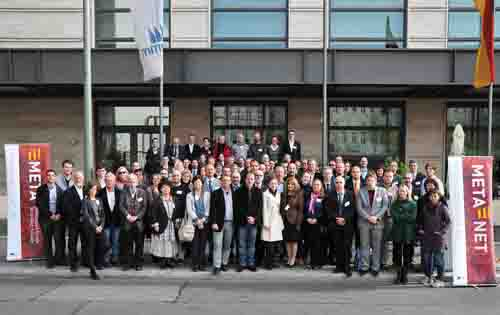
\includegraphics[width=\textwidth]{../_media/meta-net_team.jpg}
  \caption{Prop de 100 experts en tecnologies del llenguatge -- representants dels països i idiomes representats a META-NET --  van discutir i concloure els resultats clau i missatges de la sèrie de llibres blancs a la reunió de META-NET a Berlin, Alemanya el 21/22 d'octubre de 2011. ---
 \textcolor{grey1}{About 100 language technology experts -- representatives of the countries and languages represented in META-NET -- discussed and finalised the key results and messages of the White Paper Series at a META-NET meeting in Berlin, Germany, on October 21/22, 2011.}}
  \medskip
  \colorrule{grey3}{\textwidth}{1.5pt}
\end{figure*}

\cleardoublepage

\bsection[La sèrie de llibres blancs de META-NET -- The META-NET White Paper Series]{La sèrie de llibres blancs de META-NET --- The META-NET\ \ \ \ \ \ White Paper Series}
\label{whitepaperseries}

\vspace*{-5mm}
\centering
  \setlength{\tabcolsep}{2em}
  \begin{tabularx}{\textwidth}{lllll} \toprule\addlinespace
  %\begin{tabulary}{170mm}{LLL} \toprule
  Alemany & German & Deutsch\\
  Anglès & English & English\\
  Basc & Basque & euskara\\
  Búlgar & Bulgarian & български \\
  Català & Catalan & català\\
  Croat & Croatian & hrvatski\\
  Danès & Danish & dansk\\
  Eslovac & Slovak & slovenčina\\
  Eslovè & Slovene & slovenščina\\
  Espanyol & Spanish & español\\
  Estonià & Estonian & eesti\\
  Finès & Finnish & suomi\\
  Francès & French & français\\
  Gallec & Galician & galego\\
  Grec & Greek & ελληνικά\\
  Holandès & Dutch & Nederlands\\
  Hongarès & Hungarian & magyar\\ 
  Irlandès & Irish & Gaeilge\\
  Islandès & Icelandic & íslenska\\
  Italià & Italian & italiano\\
  Letó & Latvian & latviešu valoda\\
  Lituà & Lithuanian & lietuvių kalba\\
  Maltès & Maltese & Malti\\
  Noruec Bokmål & Norwegian Bokmål & bokmål\\
  Noruec Nynorsk & Norwegian Nynorsk & nynorsk\\
  Polonès & Polish & polski\\
  Portuguès & Portuguese & português\\
  Romanès & Romanian & română\\
  Serbi & Serbian & српски\\
  Suec & Swedish & svenska\\
  Txec & Czech & čeština\\  \addlinespace \bottomrule
\end{tabularx}
